\begin{frame}[containsverbatim]
\frametitle{What is HPC ?}

\begin{block}{Definition}
It is \textbf{High Performance Computing}...
\end{block}

\begin{block}{}
... High Performance means \textbf{minimizing TTS (Time To Solution)}
\end{block}

\begin{center}
\textbf{Why ?}
\end{center}
\end{frame}


\begin{frame}[containsverbatim]
\frametitle{Why more performance ?}
\begin{columns}[c]
	\begin{column}{5cm}
	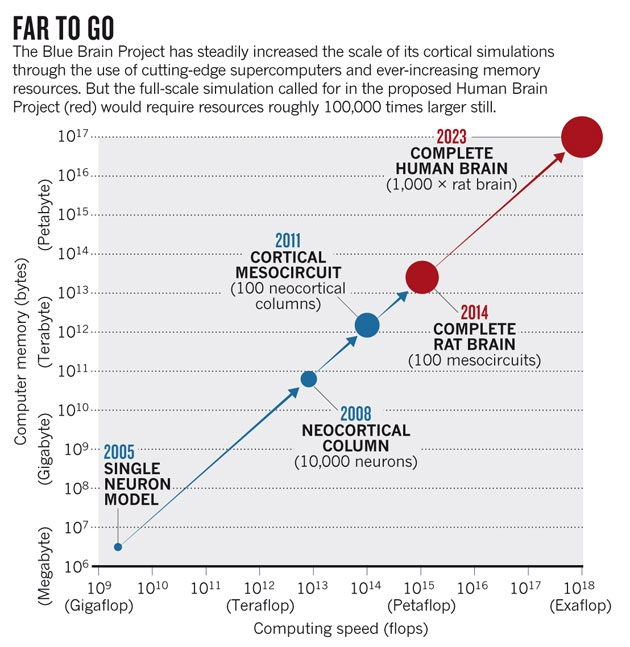
\includegraphics[width=5cm]{DayGilles/images/far-to-go.jpg}
	\end{column} 
	\begin{column}{5cm}
	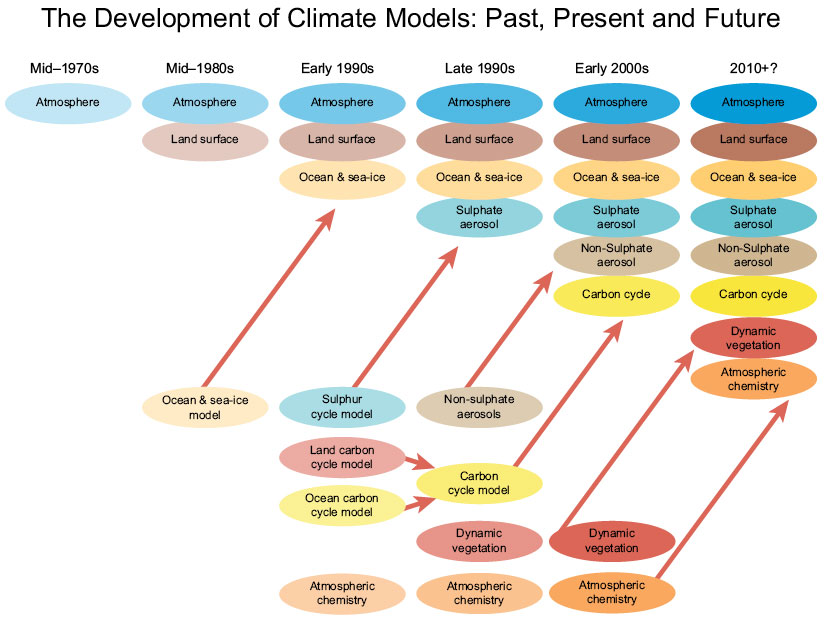
\includegraphics[width=5cm]{DayGilles/images/climatemodel.jpg}
	\end{column}
\end{columns} 

\end{frame}



\begin{frame}[containsverbatim]
\frametitle{HPC First principles: Latency and Throughput}
\begin{columns}[c]
	\begin{column}{5cm}
	\begin{alertblock}{Latency}
	Time to complete an operation
	\end{alertblock}
	\begin{alertblock}{Throughput}
	How many operations per time
	\end{alertblock}
	Water pipes analogy:
	\begin{itemize}
	\item Latency is how long it takes to water to go through the pipe
	\item Throughput is the amount of water the pipe is outputting
	\end{itemize}

	\end{column} 
	\begin{column}{5cm}
	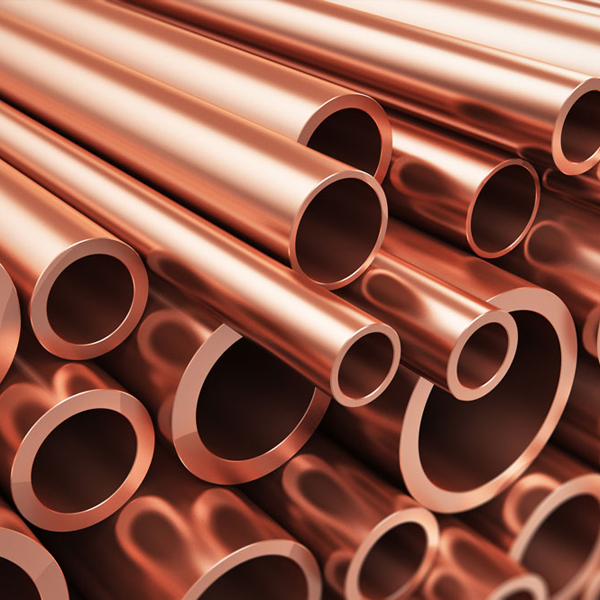
\includegraphics[width=5cm]{DayGilles/images/waterpipes.jpg}
	\end{column}
\end{columns} 
\end{frame}


\begin{frame}[containsverbatim]
\frametitle{HPC First principles: Latency and Throughput}
\begin{columns}[c]
	\begin{column}{5cm}
	Remarks:
	\begin{itemize}
	\item Cutting the pipe in half will halve the latency but throughput remains unchanged
	\item Adding a pipe does not change the latency but increases the throughput
	\end{itemize}
	\begin{alertblock}{Warning !}
	Easily confused (they refer to speed) and often contradict each other.
	\end{alertblock}
	In fact : they \textbf{relate to each other} (See Little's law : $L = \Lambda W$)
	\end{column} 
	\begin{column}{5cm}
	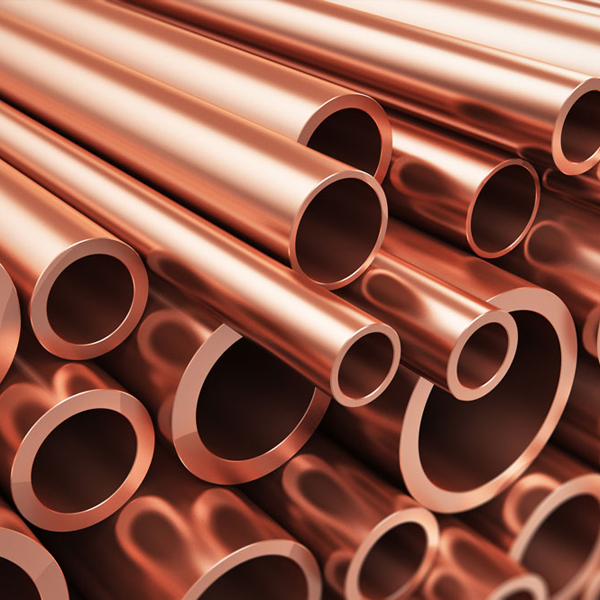
\includegraphics[width=5cm]{DayGilles/images/waterpipes.jpg}
	\end{column}
\end{columns} 
\end{frame}


\begin{frame}[containsverbatim]
\frametitle{Little's Law}
\begin{columns}[c]
	\begin{column}{5cm}
	\textbf{parallelism = latency * throughput}
	\\
	or
	\\
	\textbf{latency = parallelism / throughput}
	\\
	or
	\\
	\textbf{throughput = parallelism / latency}
	\\
	\textcolor{red}{i.e. latency is covered by parallelism !}
	\end{column} 
	\begin{column}{5cm}
	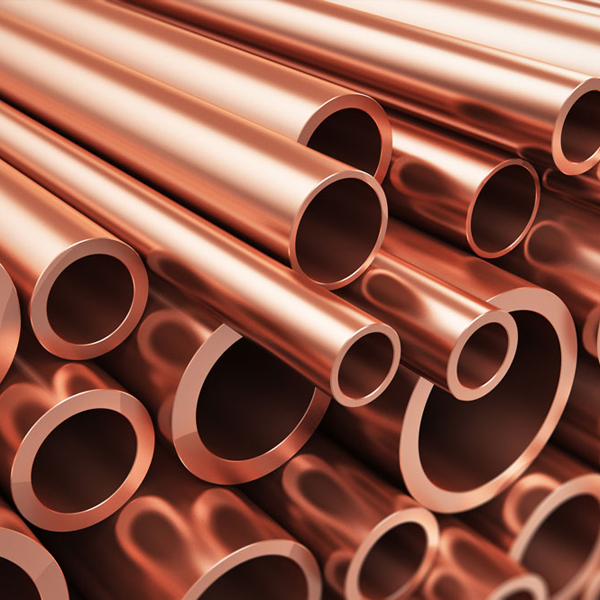
\includegraphics[width=5cm]{DayGilles/images/waterpipes.jpg}
	\end{column}
\end{columns} 
\end{frame}




\begin{frame}[containsverbatim]
\frametitle{HPC First principles: Latency and Throughput}
In general, latency reduction hits physical limits
\vfill

\begin{columns}[c]
	\begin{column}{5cm}
	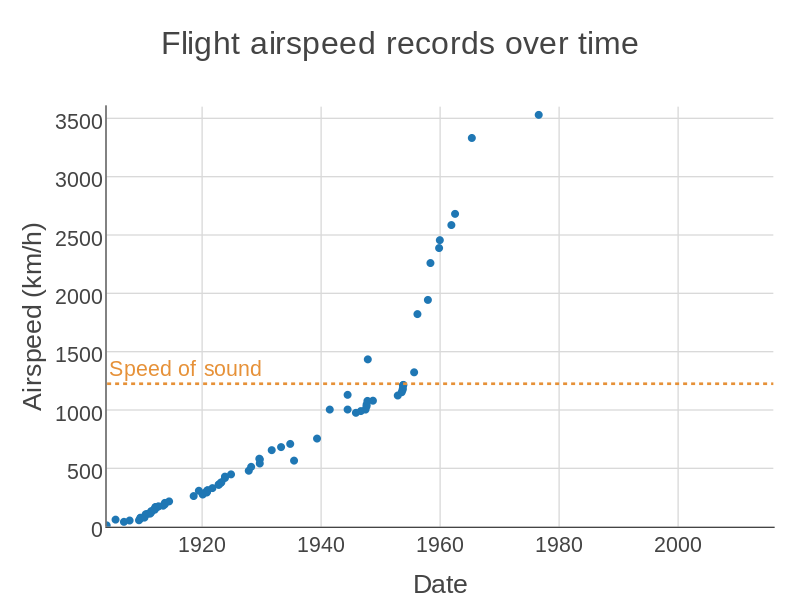
\includegraphics[width=5cm]{DayGilles/images/airspeed.png}
	\end{column} 
	\begin{column}{5cm}
	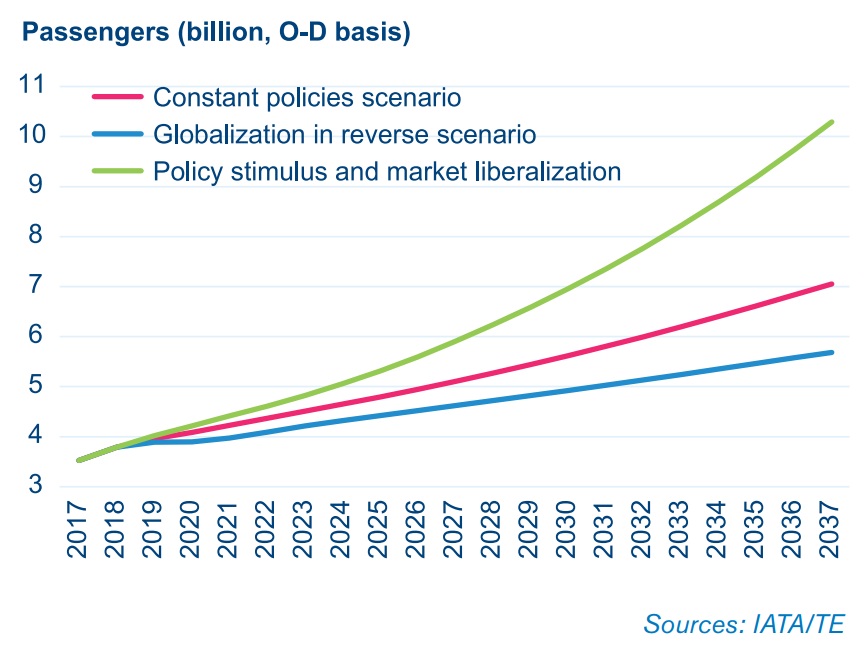
\includegraphics[width=5cm]{DayGilles/images/airtravel.png}
	\end{column}
\end{columns} 
\vfill
Planes do not fly faster, but they are much more in the sky.
\end{frame}



\begin{frame}[containsverbatim]
\frametitle{Latency and Throughput for CPUs}

\begin{alertblock}{\textbf{Latency} (in seconds or cycles)}
how long it takes before the next dependent operation can start. \textbf{The dependent operation's performance is limited by latency}
\end{alertblock}
\vfill

\begin{alertblock}{\textbf{Throughput} (in instructions per cycle or per second)}
number of independent operations per time unit. \textbf{The independent operation's performance is limited by the throughput}
\end{alertblock}

\end{frame}



\begin{frame}[containsverbatim]
\frametitle{HPC First principles: Memory latency and throughput}
Memory bandwidth goes up (nice !) but latency does not go down (not so nice !)
\begin{center}
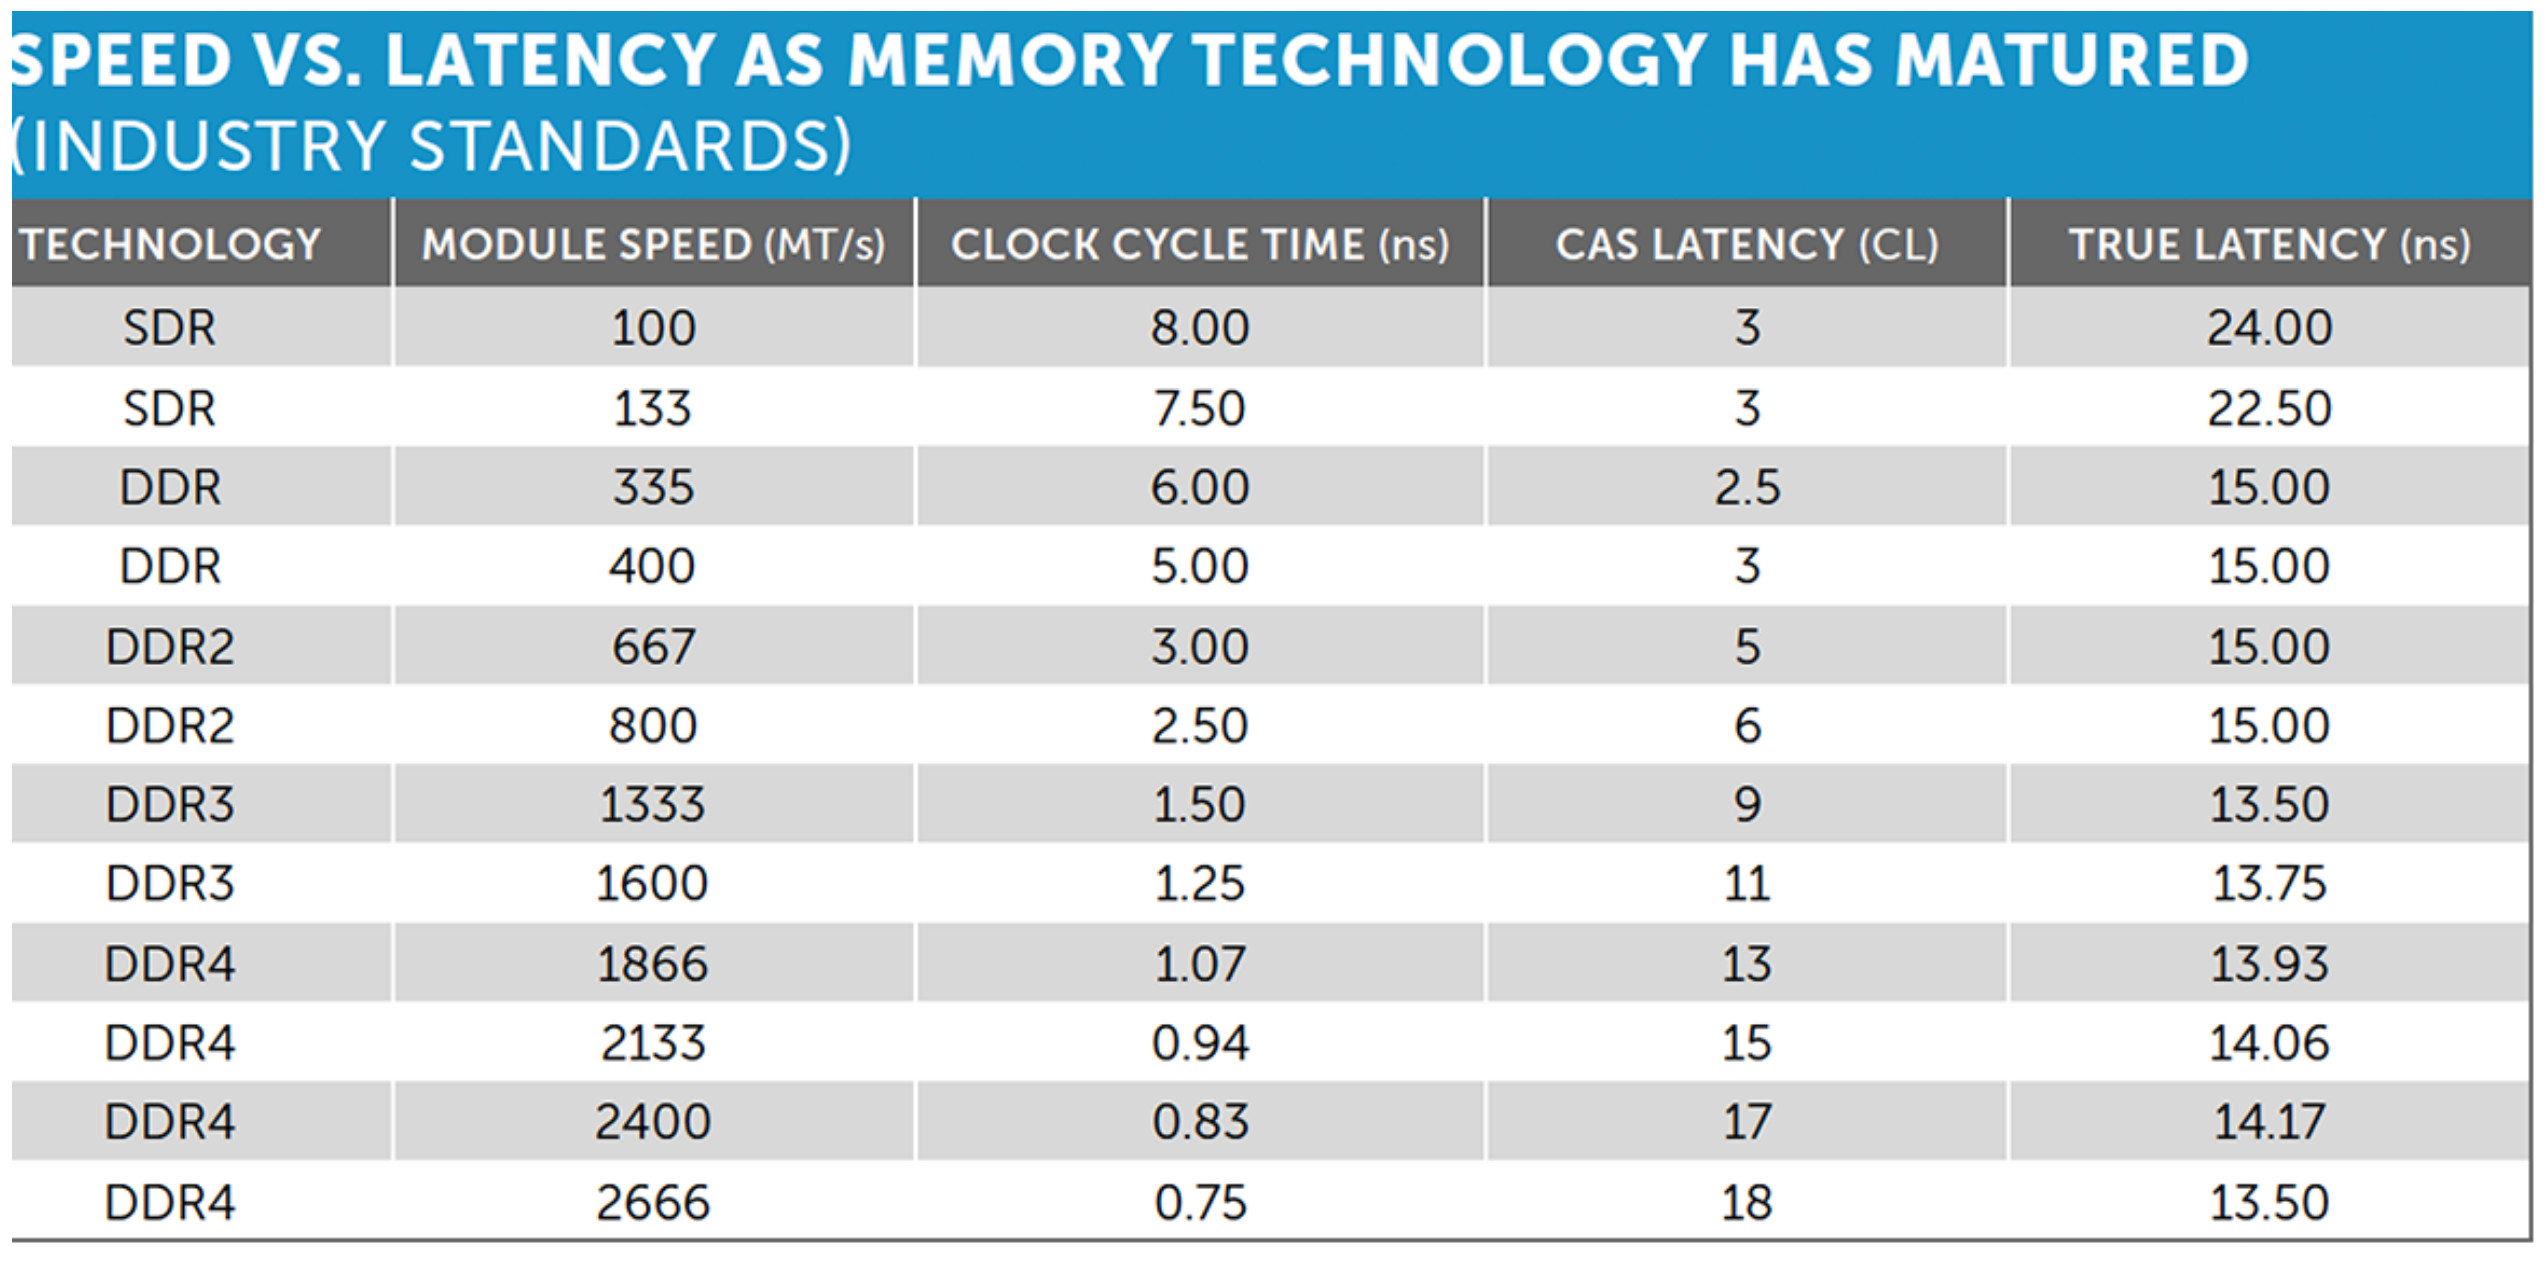
\includegraphics[width=10cm]{DayGilles/images/memory.jpg}
\end{center}
\end{frame}


\begin{frame}[containsverbatim]
\frametitle{HPC First principles: Memory latency and throughput}
Memory prefetchers : increasing throughput by maximizing data locality
\vfill

\begin{columns}[b]
	\begin{column}{6cm}
	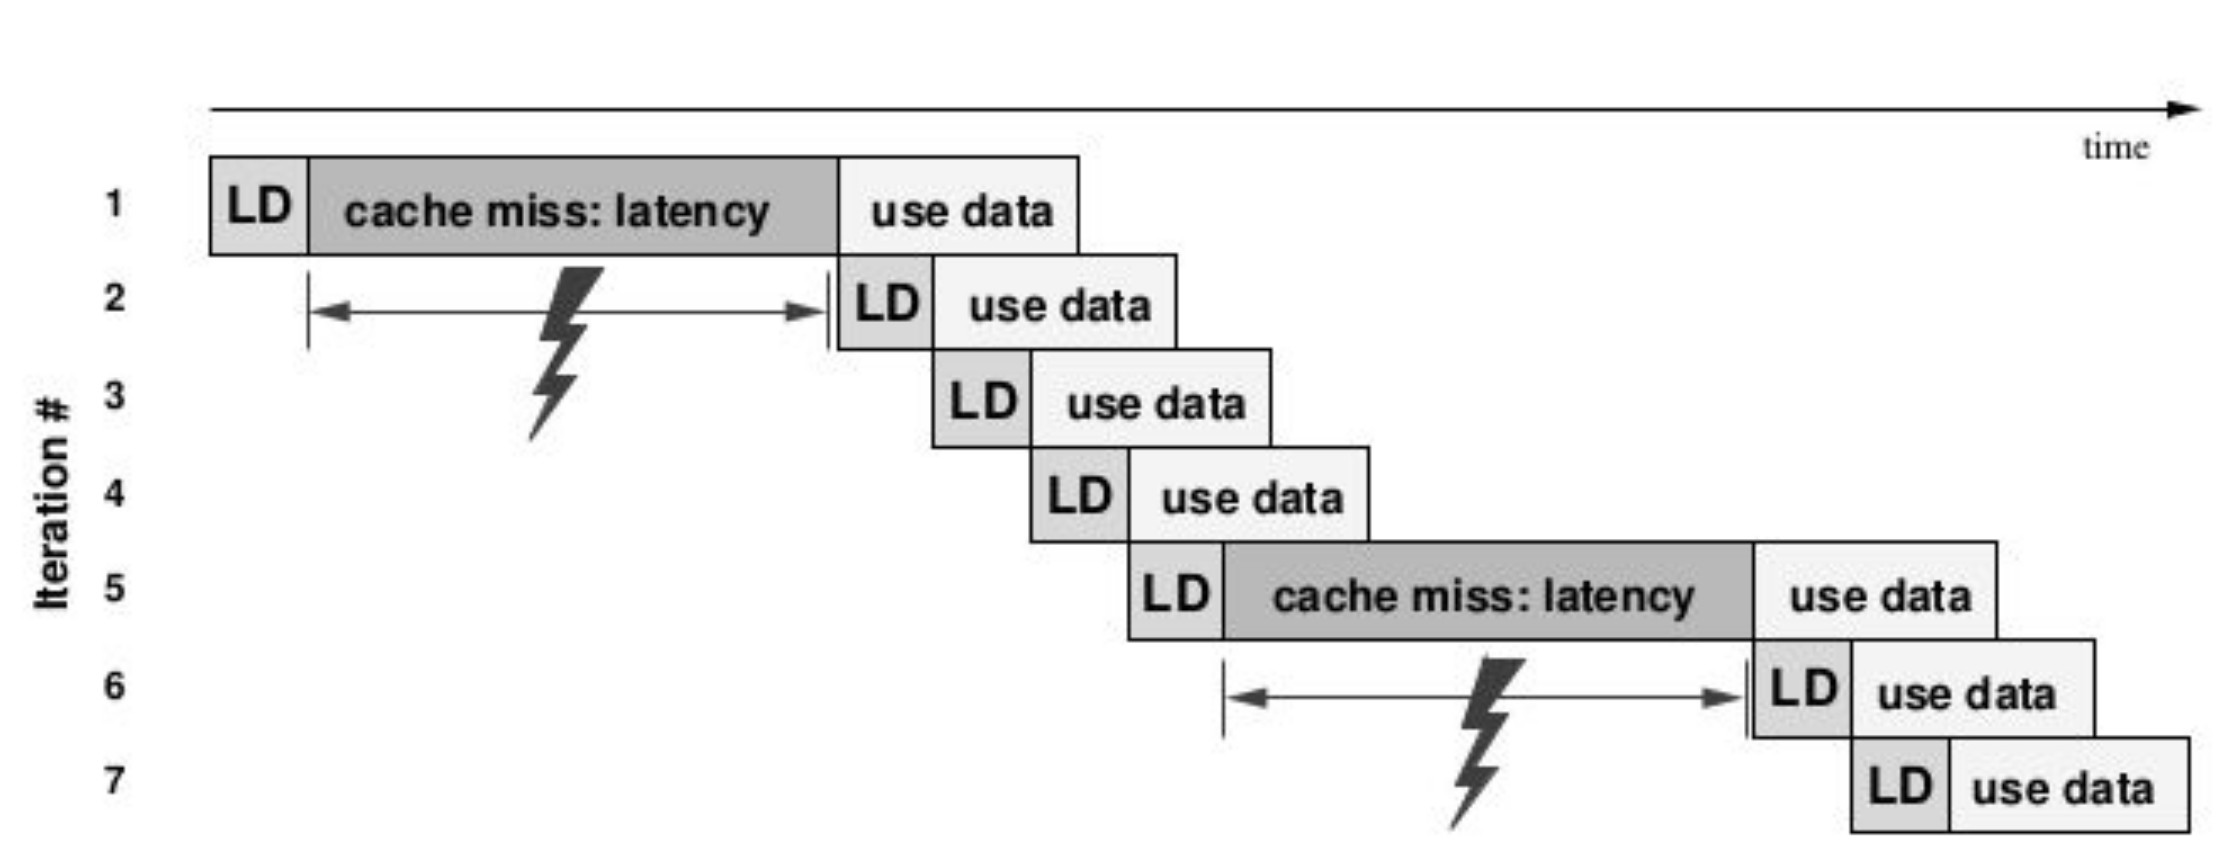
\includegraphics[width=6cm]{DayGilles/images/prefetch-latency.jpg}
	\\
	Latency bound
	\end{column} 
	\begin{column}{4cm}
	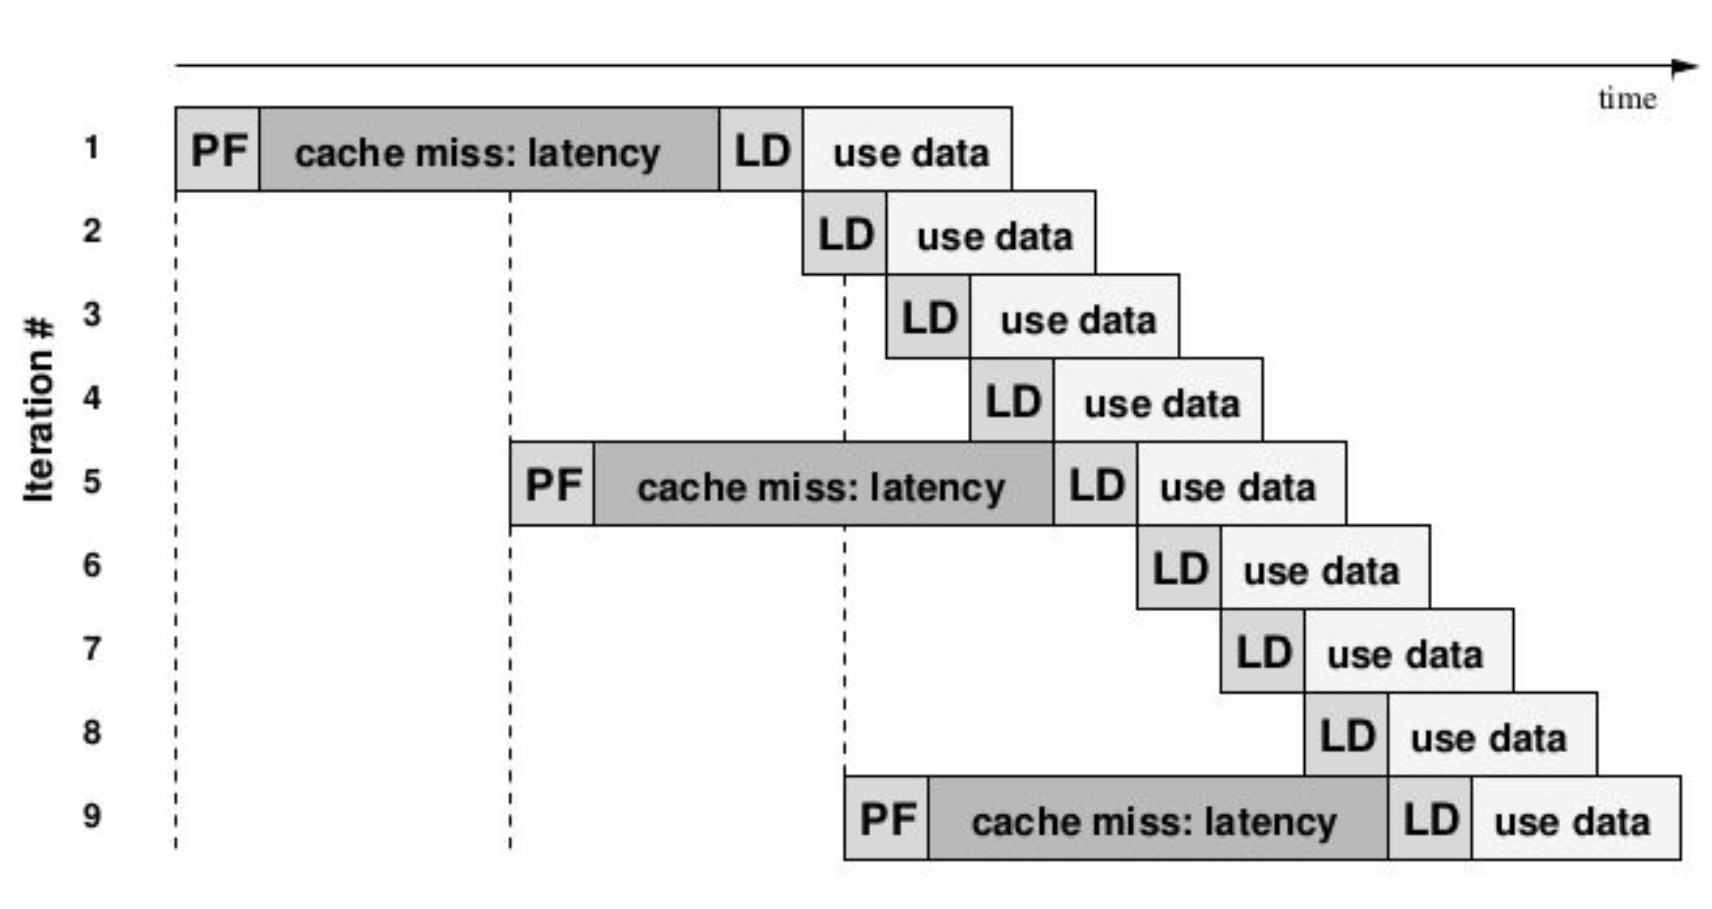
\includegraphics[width=4cm]{DayGilles/images/prefetch-bandwidth.jpg}
	\\
	Bandwidth bound
	\end{column}
\end{columns} 
\vfill
The CPU need to know where to fetch the data :
\begin{itemize}
	\item contiguous accesses will maximize the throughput
	\item non-contiguous accesses are latency bound
\end{itemize}
\end{frame}



\begin{frame}[containsverbatim]
\frametitle{Math operations : latency and throughput}

\begin{center}
\begin{table}
\resizebox{\textwidth}{!}{%
\begin{tabular}{|l|r|r|r|r|r|r|} 
\hline
 & \multicolumn{2}{c|}{Broadwell} & \multicolumn{2}{c|}{KNL} & \multicolumn{2}{c|}{Kepler GPU} \\
\hline
Math Op & LAT (C) & TP (IPC) & LAT (C) & TP (IPC) & LAT (C) & TP (IPC) \\
\hline
Add & 3 & 1 & 2  & 2 & 9 & ? \\
\hline
Multiply & 3 & 2 & 7  & 2 & 9 & ? \\
\hline
FMA & 5 & 2 & 6 & 2 & 9 & 32(?) \\
\hline
Division & 10-14 & 0.05 & 32 & 0.031 & 141 & ? \\
\hline
Sqrt & 10-23 & 0.2 & 38 & 0.063 & 181 & ? \\
\hline
Sin/Cos & 52-124 & ? & 50-250 & 0.006 & 18 & ? \\
\hline
Atan & 97-147 & ? & 125-265 & 0.001 & ? & ? \\
\hline
Log & 92 & ? & 190 & 0.005 & 22 & ? \\
\hline
\end{tabular}}
\end{table}
\end{center}

As a reference, a DRAM memory access is about 200 cycles (i.e. memory wall)
\vfill

CPUs are designed to perform multiply-adds (FMA), but that's all about it. \textcolor{red}{use as many FMA as possible}
\end{frame}



\begin{frame}[containsverbatim]
\frametitle{HPC First principles: Memory latency and throughput}
\begin{center}
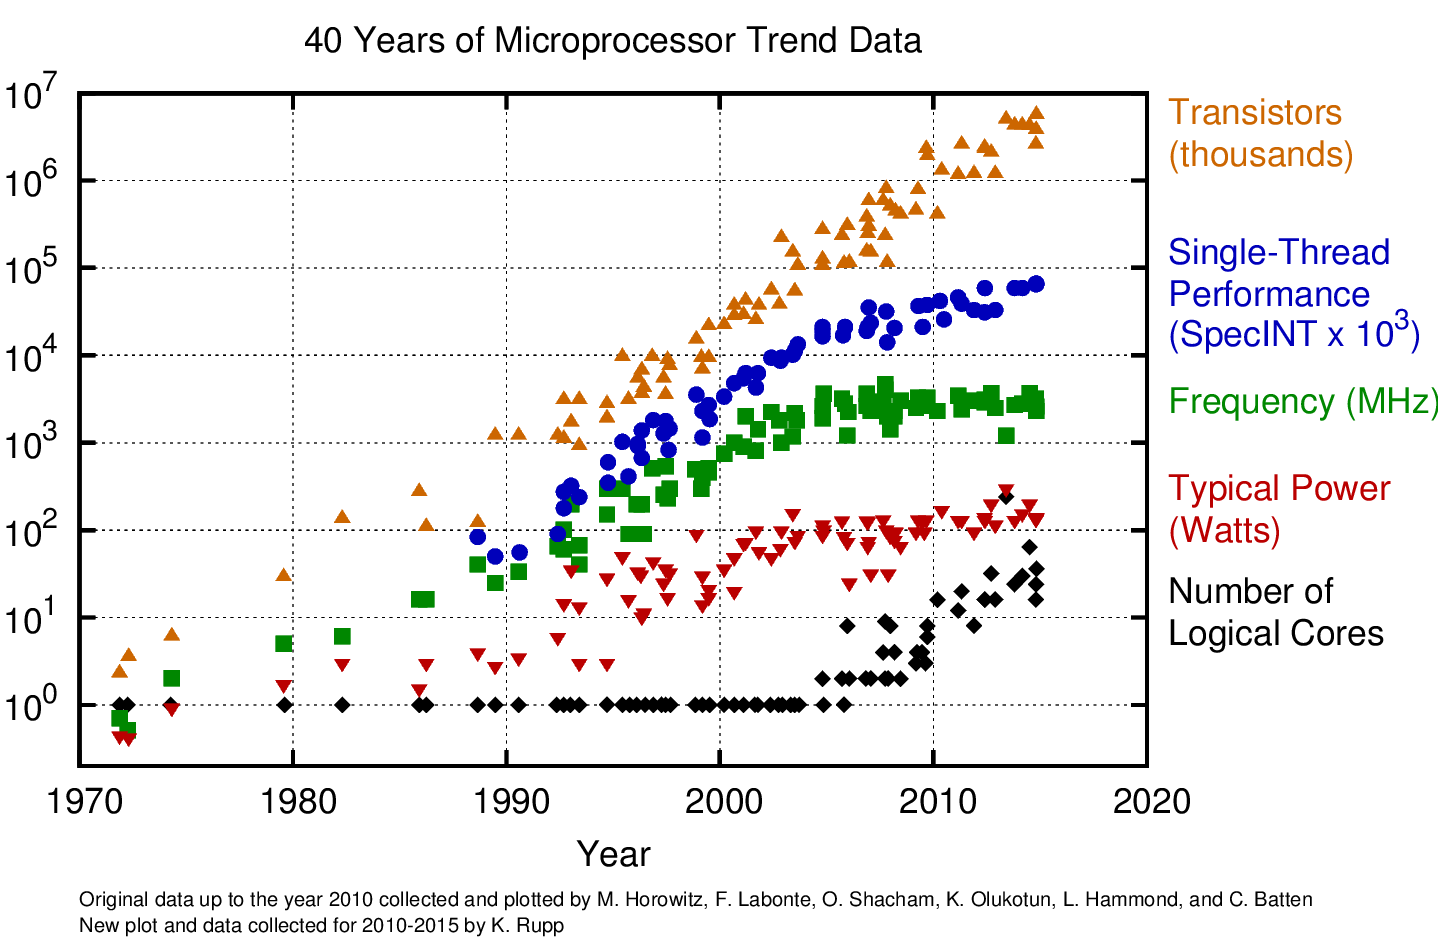
\includegraphics[width=9cm]{DayGilles/images/frequency.png}
\end{center}
CPU frequency has a hit a limit more than 10 years ago. But the performance still goes up ! \textcolor{red}{Thanks to parallel performance} (more cores)
\end{frame}


\begin{frame}[containsverbatim]
\frametitle{CPU FP (floating point) peak performance}
\begin{center}
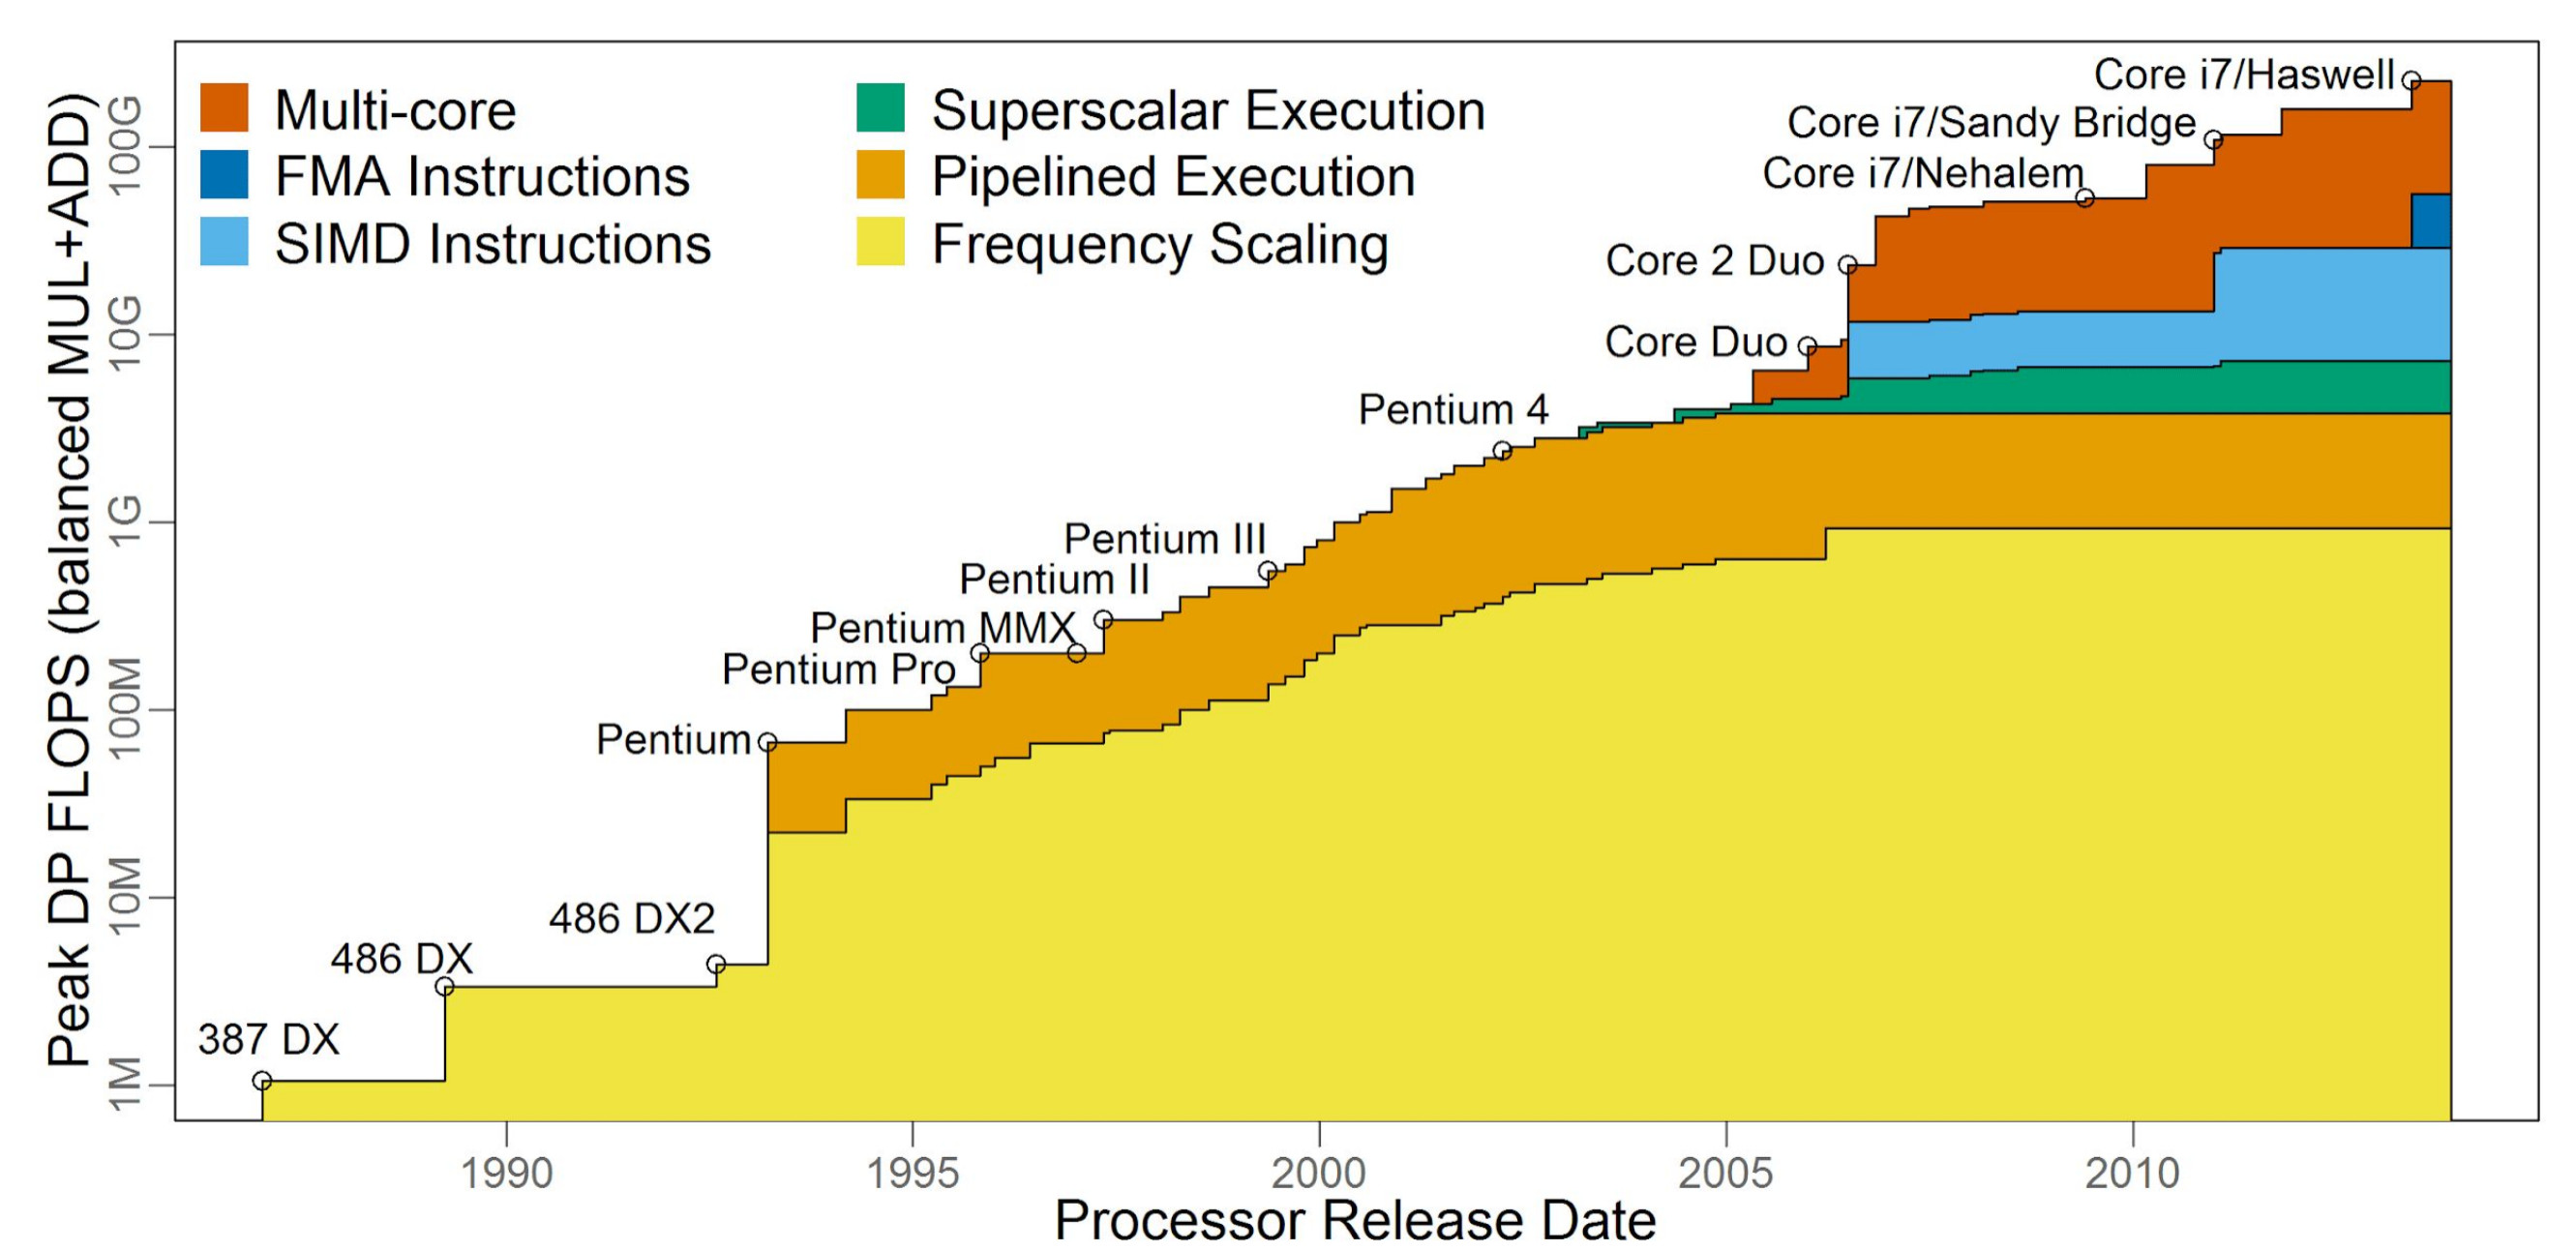
\includegraphics[width=11cm]{DayGilles/images/fp-peak.jpg}
\end{center}
\end{frame}


\begin{frame}[containsverbatim]
\frametitle{CPU FP (floating point) peak performance}
\begin{center}
\begin{alertblock}{The ninja gap}
\textbf{Question : how to benefit of the parallel features of the modern CPUs (FMA, SIMD, Pipeline, etc..) ?}
\end{alertblock}
\end{center}
\end{frame}


\begin{frame}[containsverbatim]
\frametitle{Different levels of parallelism}
\begin{center}
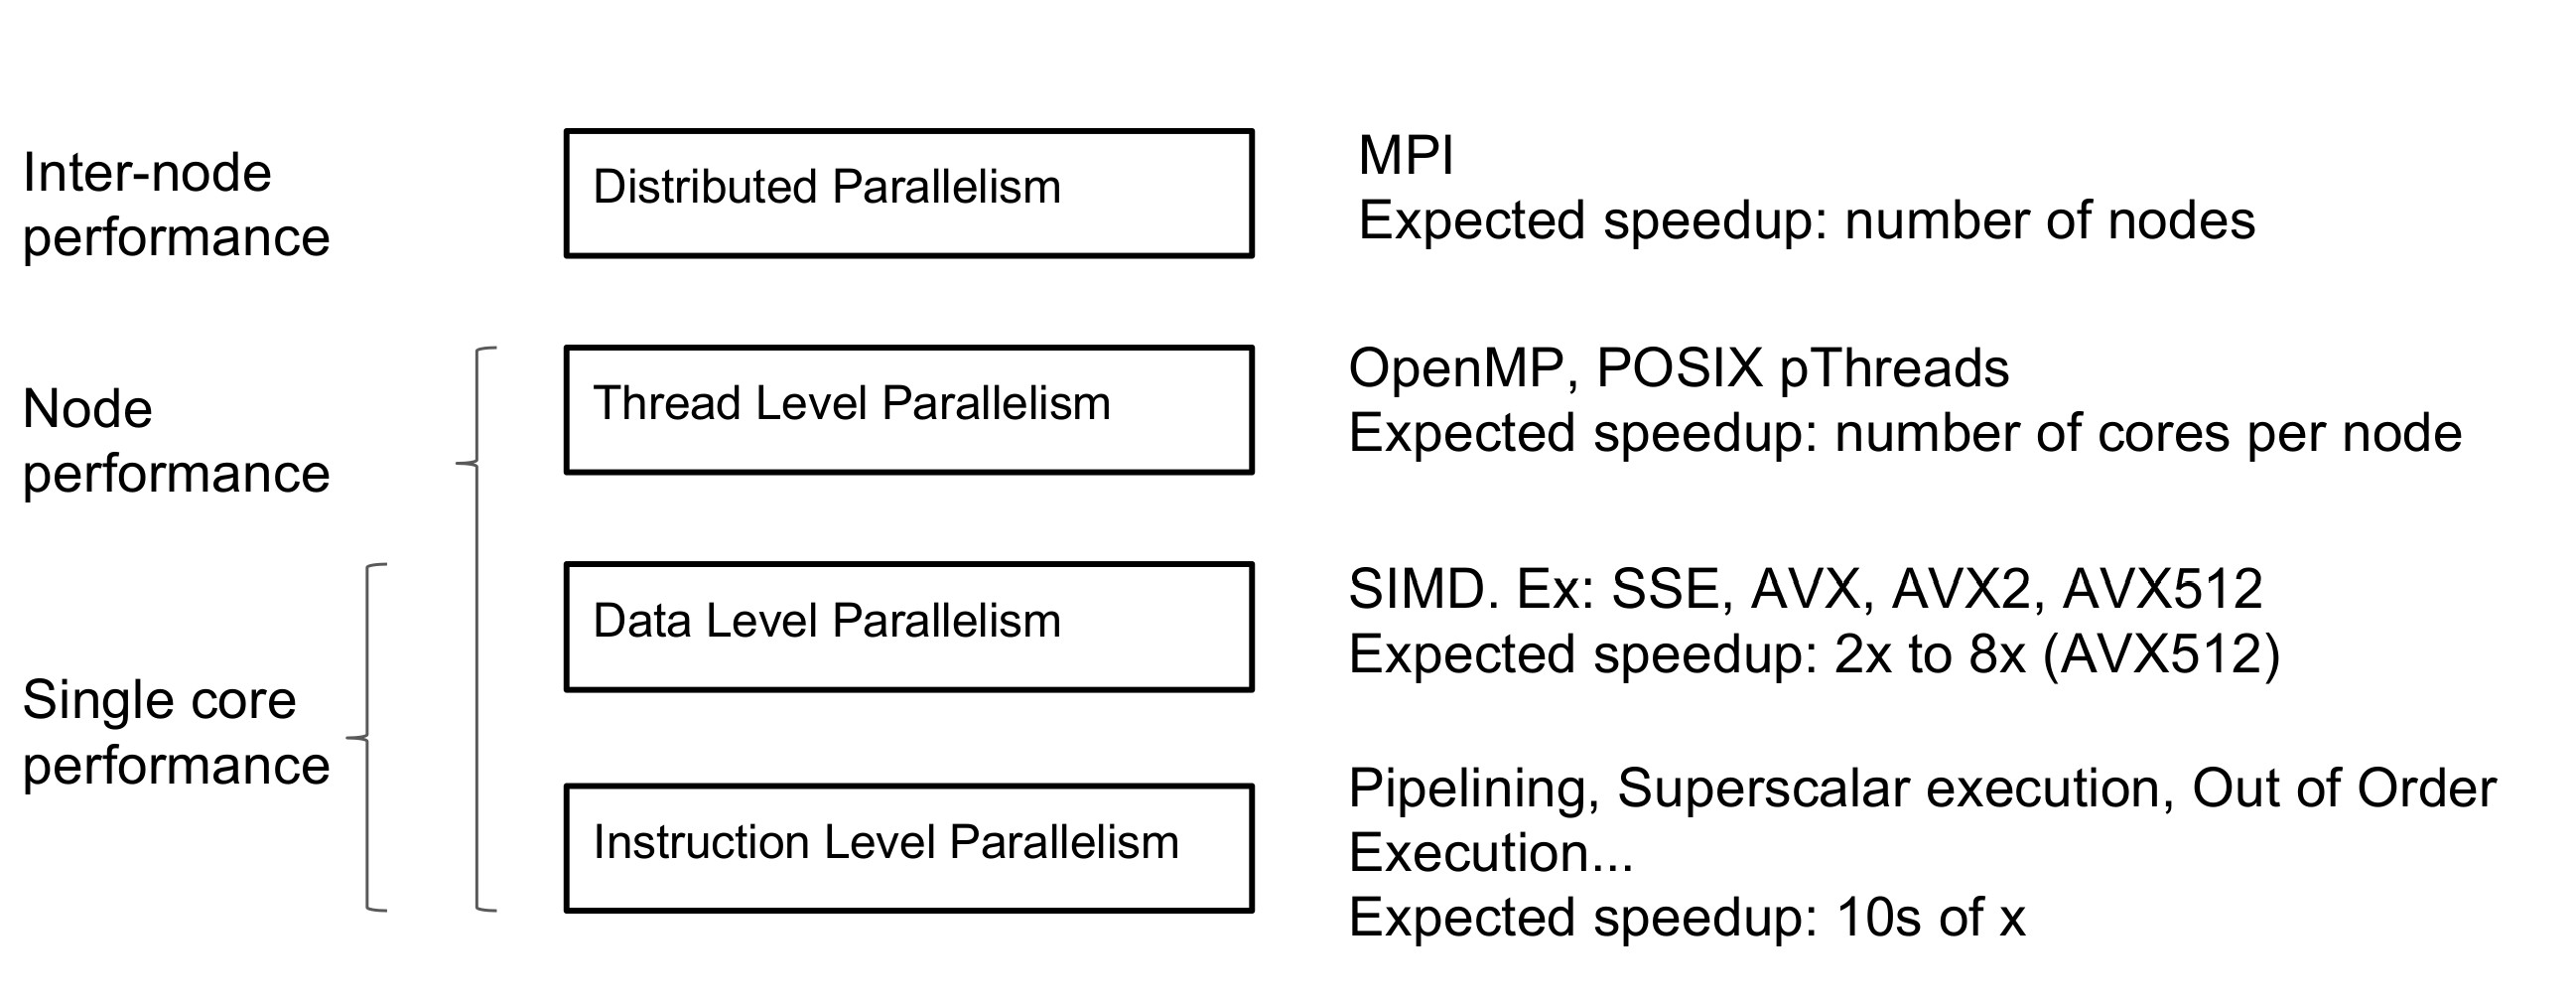
\includegraphics[width=11cm]{DayGilles/images/parallelism.jpg}
\end{center}
\vfill
Performance is based on the duplication of resources and is harnessed by parallelism.
\end{frame}


\begin{frame}[containsverbatim]
\frametitle{Instruction level parallelism (ILP)}
\begin{center}
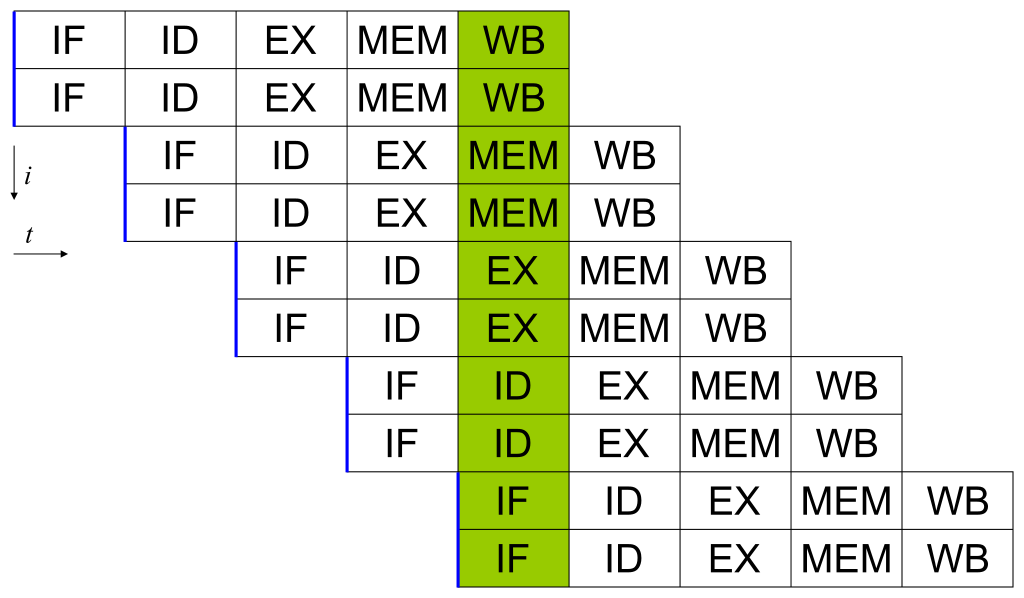
\includegraphics[width=9cm]{DayGilles/images/ilp.png}
\end{center}
\vfill
The goal is to maximize the CPU utilization and to avoid stalls. 
\end{frame}


\begin{frame}[containsverbatim]
\frametitle{Pipelining}
\begin{center}
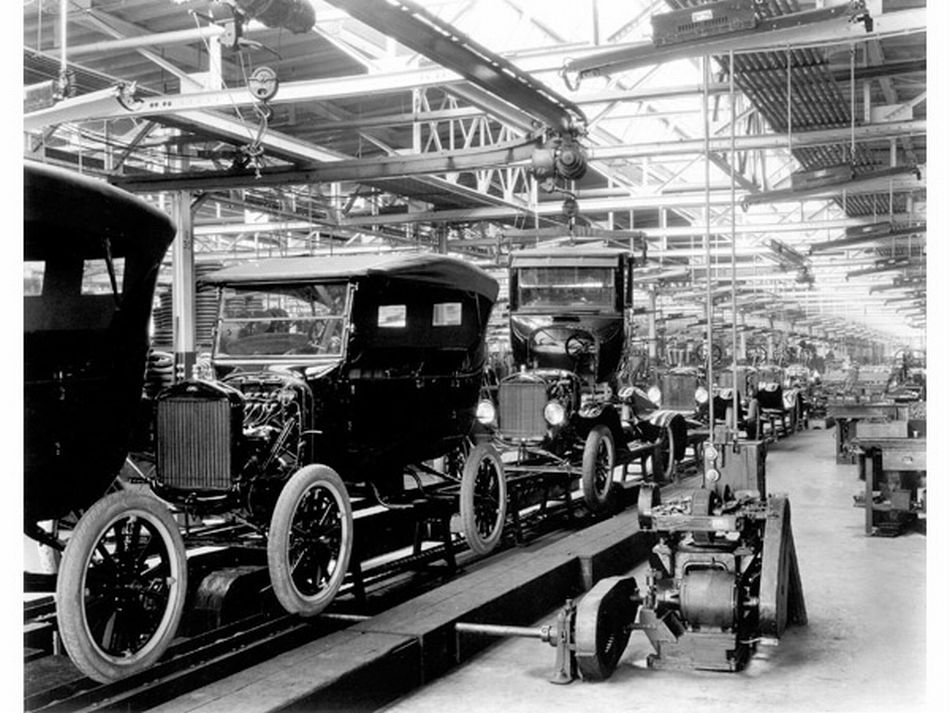
\includegraphics[width=9cm]{DayGilles/images/ford.jpg}
\end{center}
\vfill
Ford T's assembly line
\end{frame}


\begin{frame}[containsverbatim]
\frametitle{Pipelining}
Ford’s assembly line
\vfill
\textit{Ford had been trying to increase his factories’ productivity for years. The workers (...) arranged the parts in a
row on the floor, put the under-construction auto on skids and dragged it down the line as they worked. Ford
broke the Model T’s assembly into 84 discrete steps and trained each of his workers to do just one.}
\vfill
\textbf{The most significant piece of Ford’s efficiency crusade was the assembly line}
\vfill
{\tiny \url{https://www.history.com/this-day-in-history/fords-assembly-line-starts-rolling}}
\end{frame}


\begin{frame}[containsverbatim]
\frametitle{Without pipelining}
\begin{center}
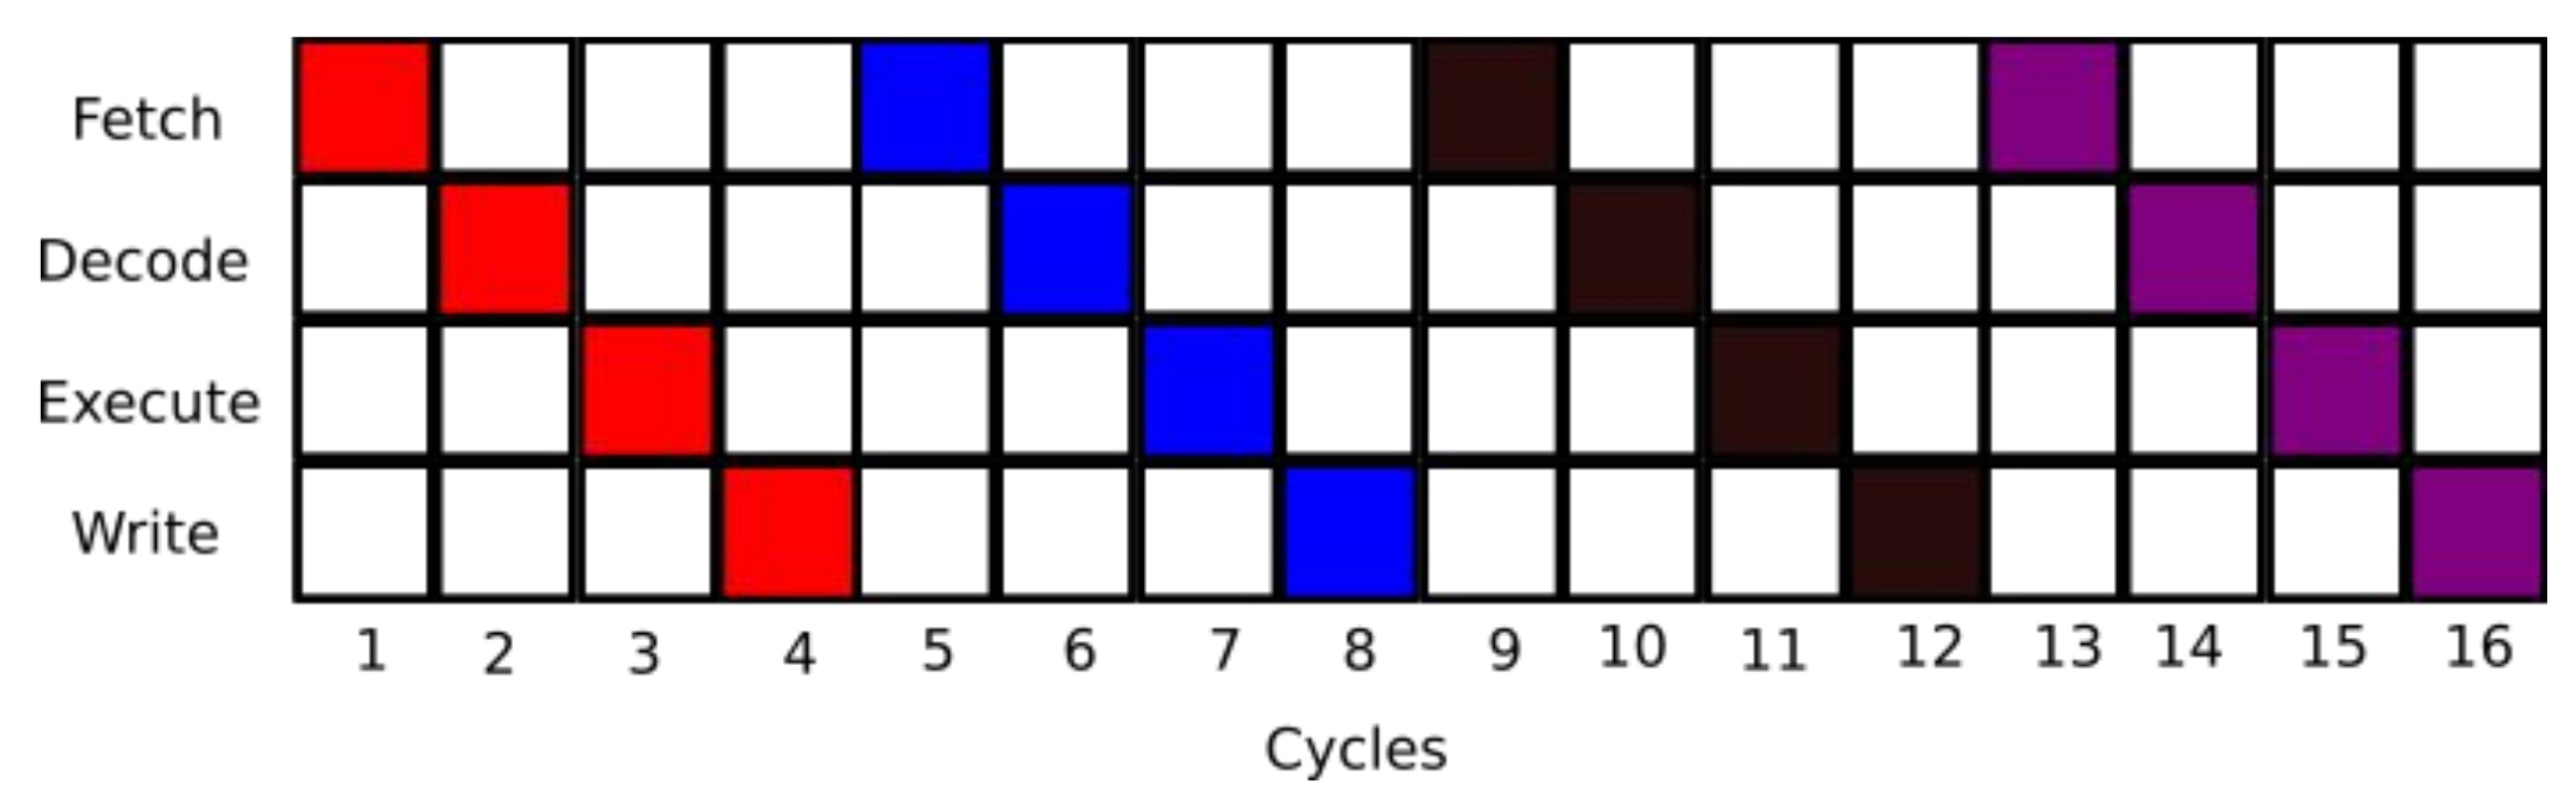
\includegraphics[width=9cm]{DayGilles/images/pipeline-without.jpg}
\end{center}
\begin{itemize}
\item 16 cycles to execute 4 instructions. Instruction latency is 4 cycles
\item Throughput is 1/4 instructions per cycle (IPC)
\end{itemize}
\end{frame}


\begin{frame}[containsverbatim]
\frametitle{Pipelining}
\begin{center}
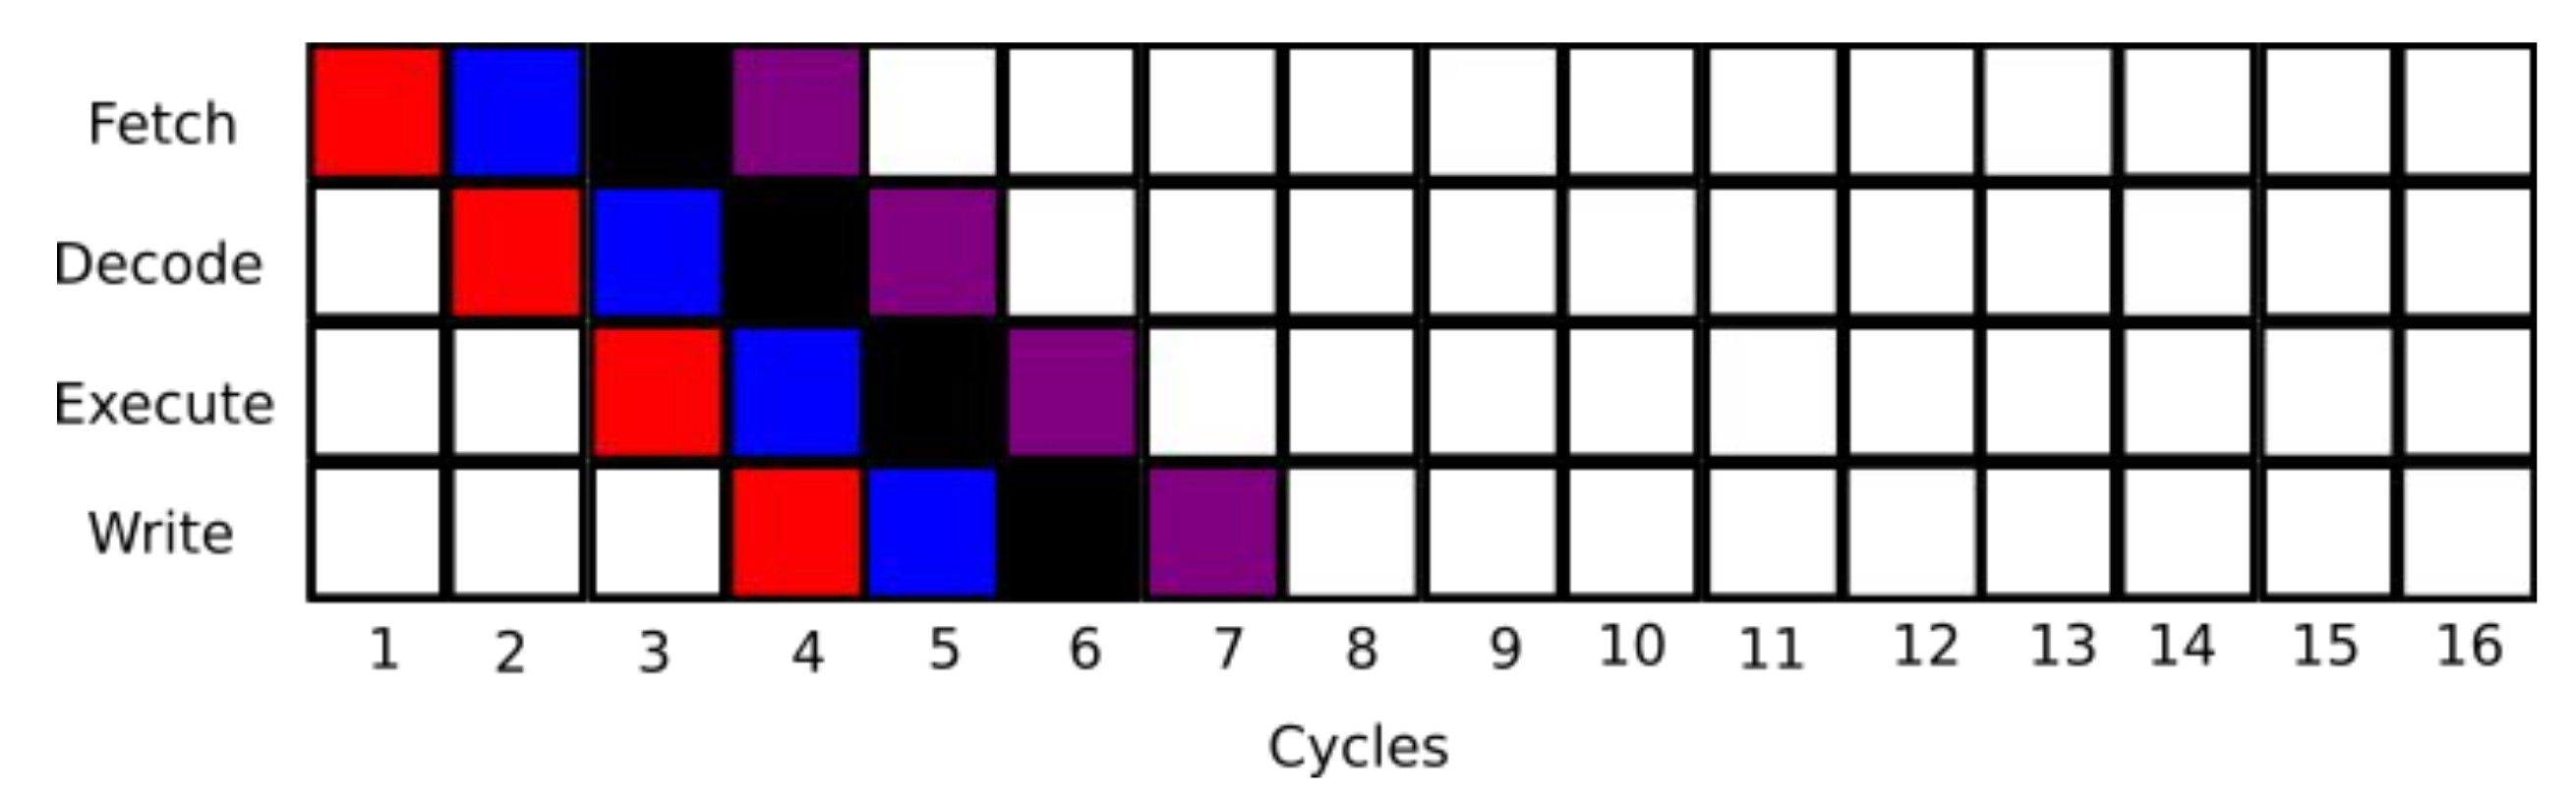
\includegraphics[width=9cm]{DayGilles/images/pipeline-with.jpg}
\end{center}
\begin{itemize}
\item 16 cycles to execute 4 instructions broken to 4 stages
\item Instruction latency is STILL 4 cycles 
\item Throughput is ~4/7 IPC, almost 2x compared to non-pipelined
\end{itemize}
\end{frame}


\begin{frame}[containsverbatim]
\frametitle{Pipelining}
Like Ford's assembly line, instructions are broken down in many small steps (stages)
\begin{itemize}
\item Increased IPC through increased parallelism
\item Smaller stages means increased frequency (which unlocked the \textit{frequency era})
\end{itemize}
But there is a price to pay: deep pipelines can easily stall
\begin{center}
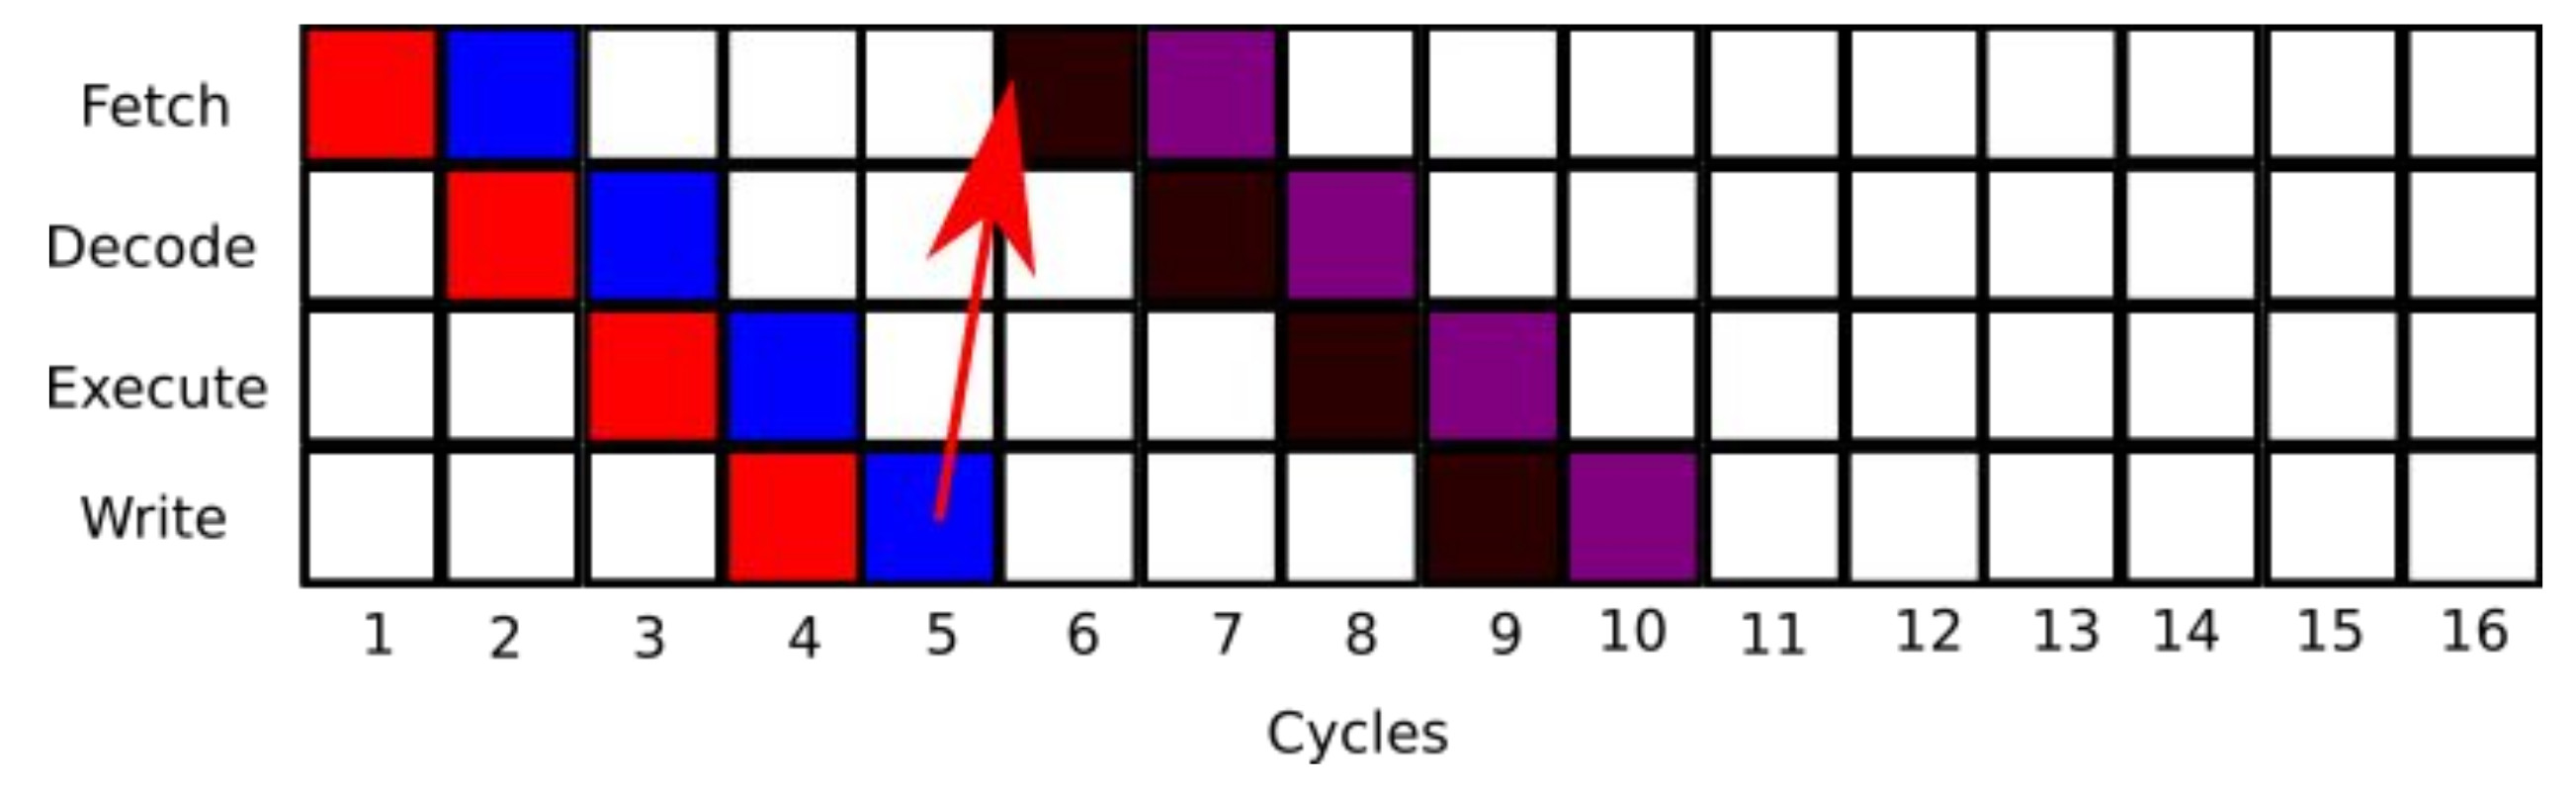
\includegraphics[width=9cm]{DayGilles/images/pipeline-stall.jpg}
\end{center}
\end{frame}


\begin{frame}[containsverbatim]
\frametitle{Pipelining}
Stalls (bubbles) happen when the pipeline cannot advance properly. Causes are :
\begin{itemize}
\item most probable instruction dependency
\item the CPU is waiting for a ressource (e.g. read/write in the memory)
\end{itemize}
\begin{center}
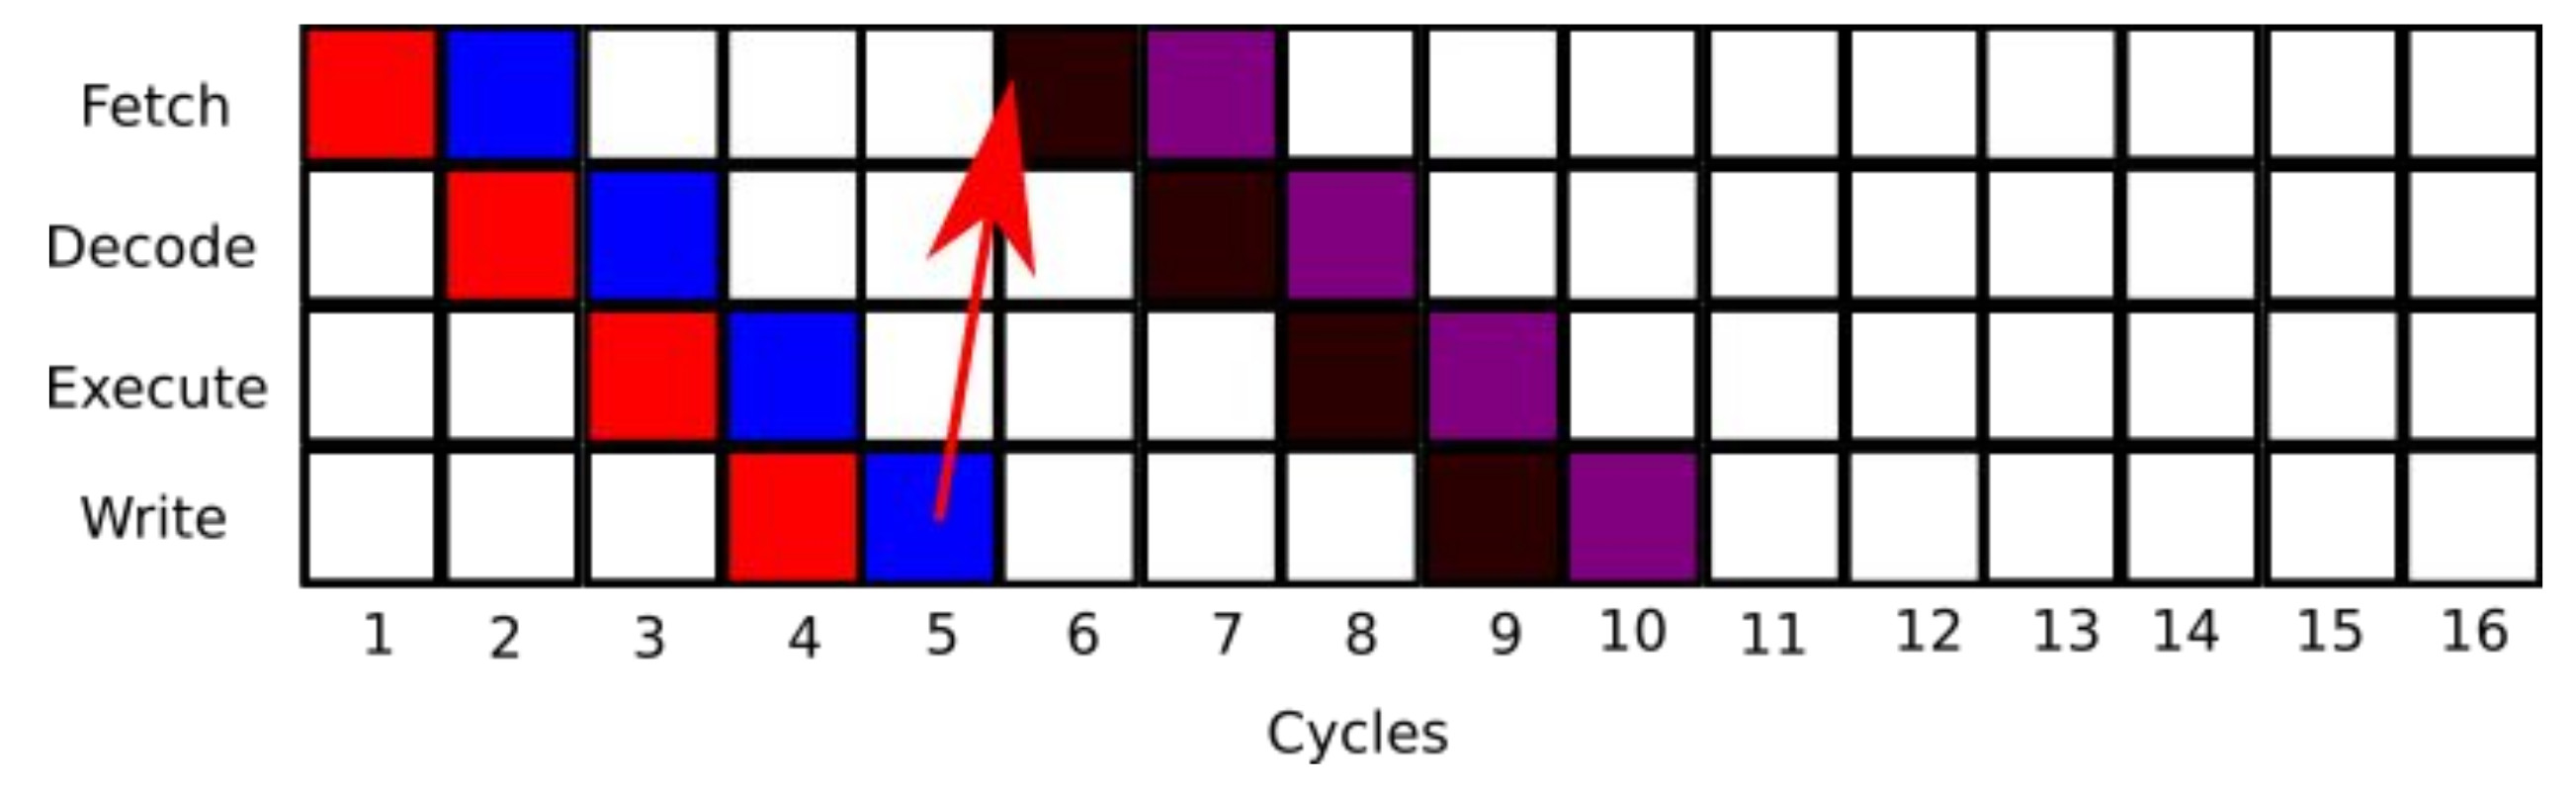
\includegraphics[width=9cm]{DayGilles/images/pipeline-stall.jpg}
\end{center}
\end{frame}


\begin{frame}[containsverbatim]
\frametitle{Superscalar architecture}
\begin{center}
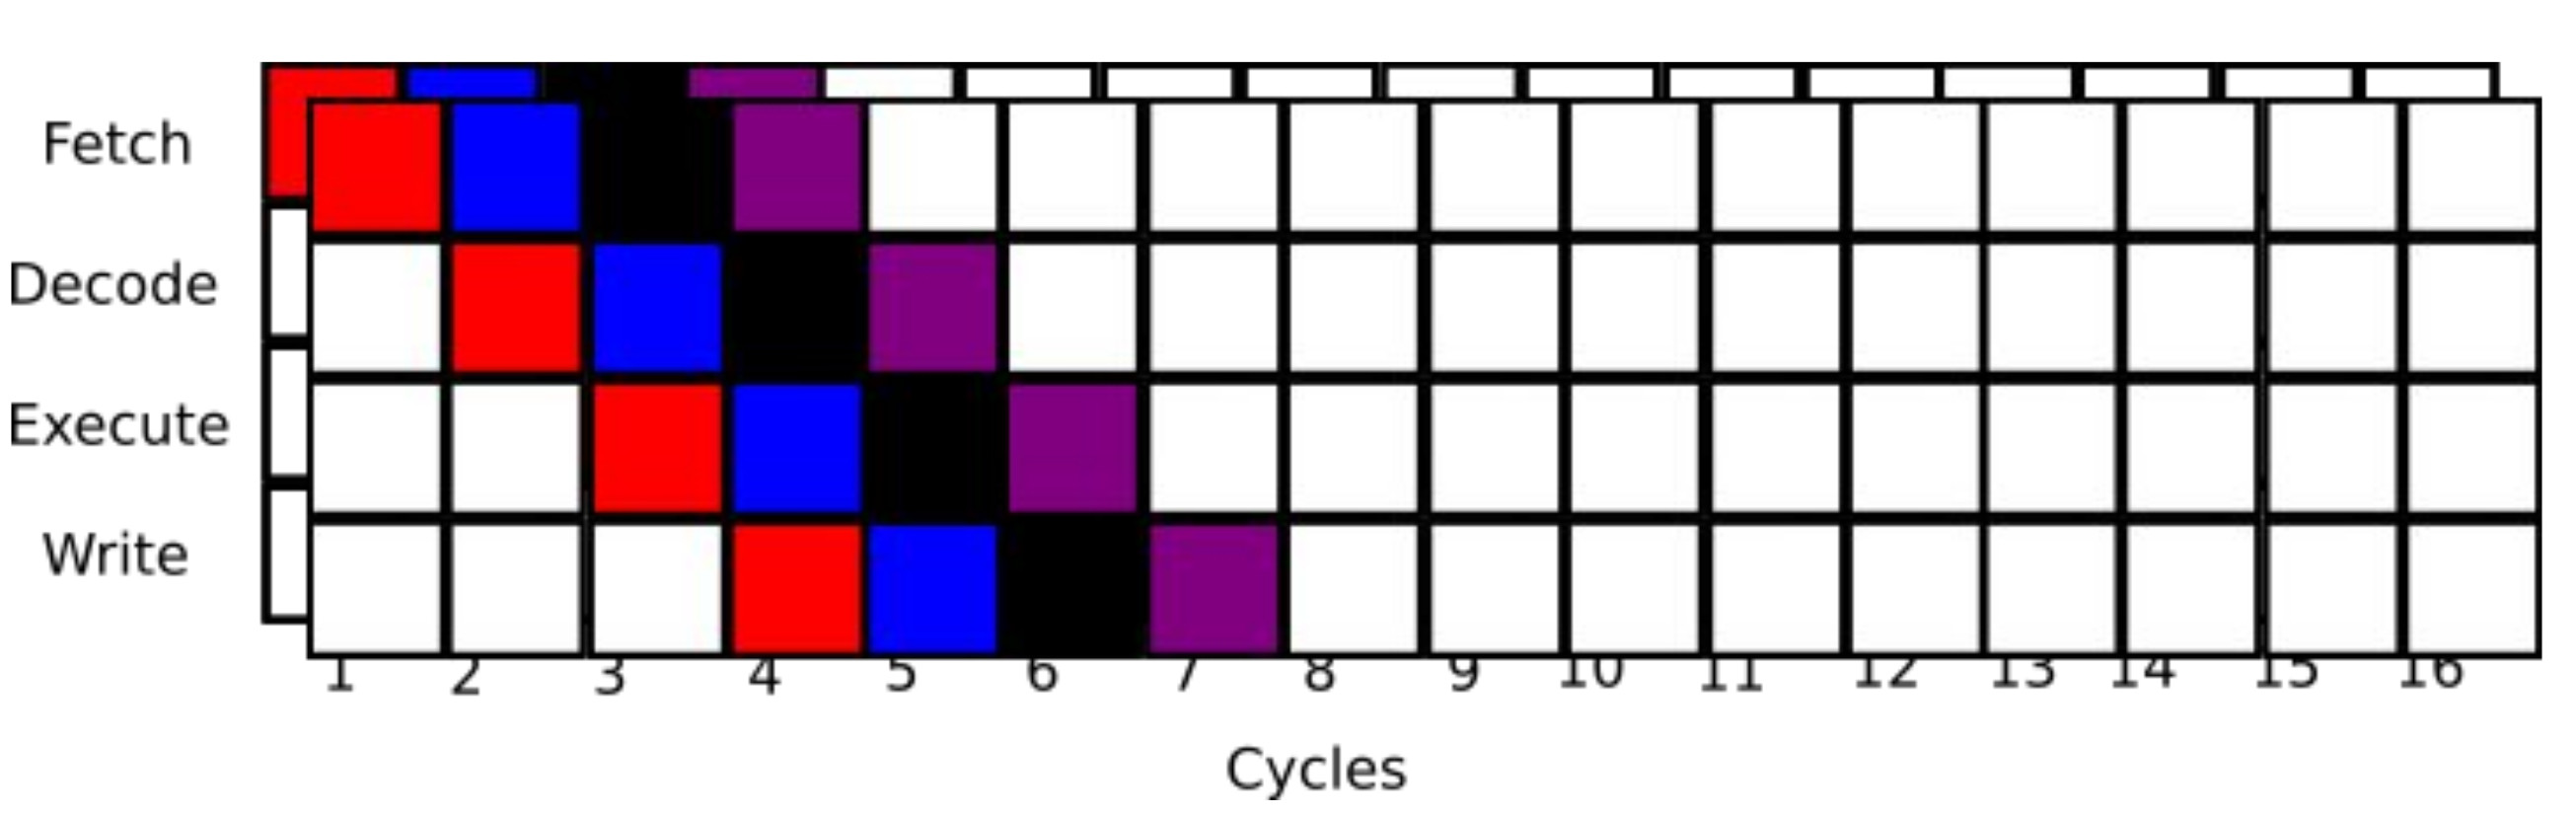
\includegraphics[width=9cm]{DayGilles/images/pipeline-superscalar.jpg}
\end{center}
\begin{itemize}
\item multiple pipelines to increase IPC
\item can be spoiled by data, control, structural hazards and multi-cycles instructions
\end{itemize}
\end{frame}


\begin{frame}[containsverbatim]
\frametitle{Out-of-order execution}
\textbf{In-Order Execution :} first instruction \textbf{in} is the first instruction executed
\vfill
\textbf{Out-Of-Order Execution :} first instruction \textbf{ready} is the first instruction executed
\begin{itemize}
\item operations are reordered
\item operations without dependencies are executed when the execution engines are ready
\item results are immediately available when needed (if the prediction was correct)
\end{itemize}
\end{frame}


\begin{frame}[containsverbatim]
\frametitle{Out-of-order execution}
\begin{center}
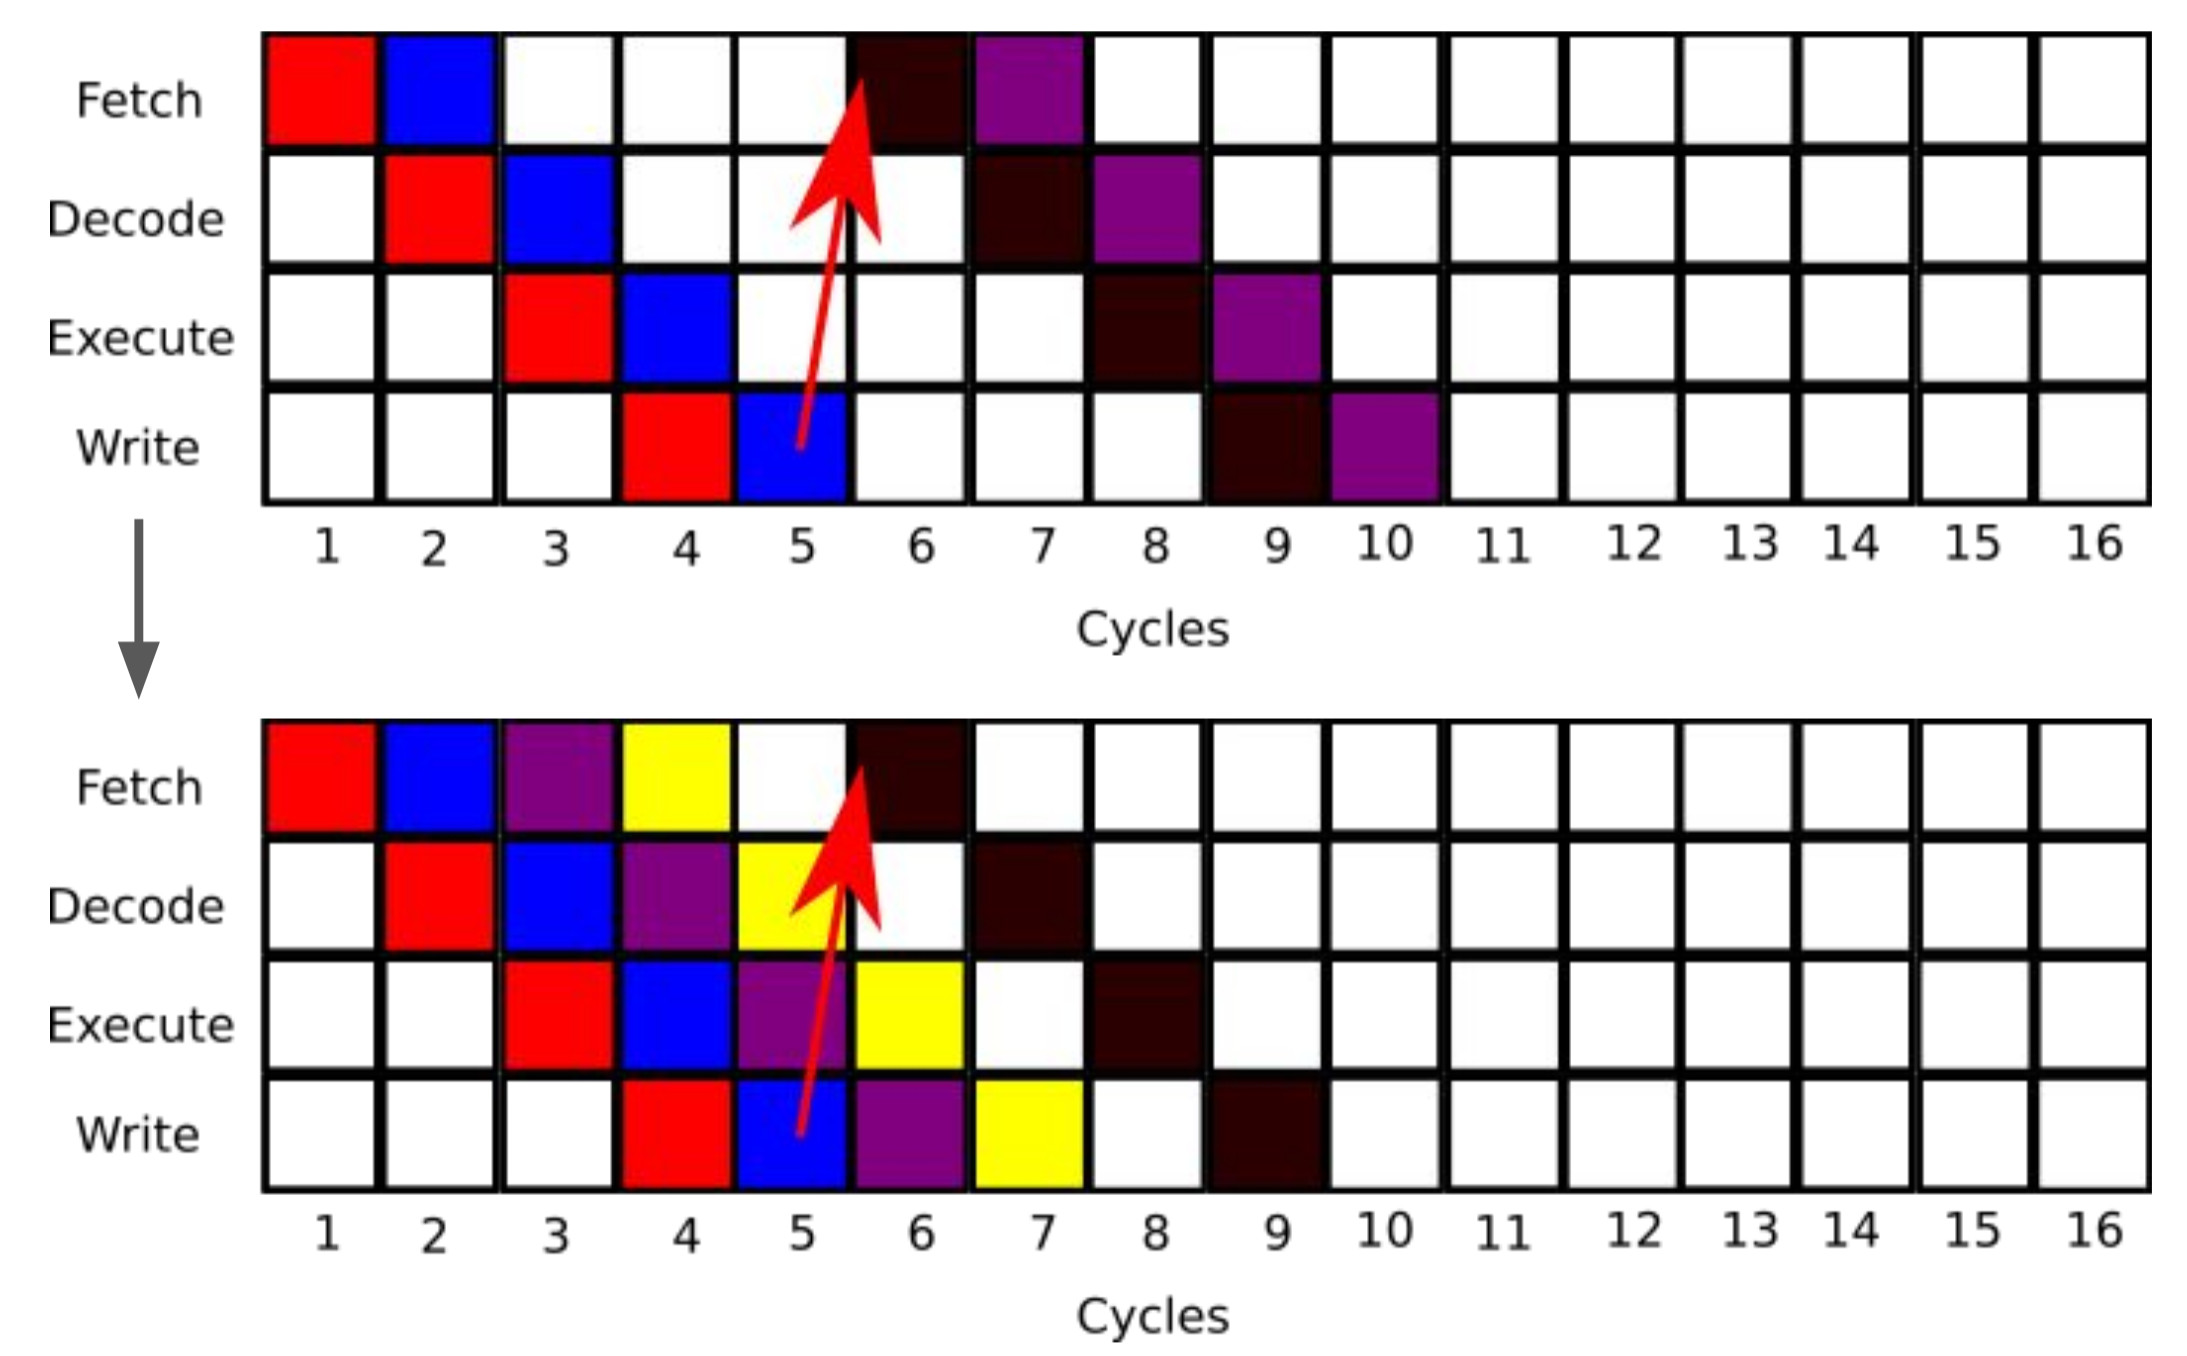
\includegraphics[width=10cm]{DayGilles/images/pipeline-outoforder.jpg}
\end{center}
\end{frame}



\begin{frame}[containsverbatim]
\frametitle{Modern CPU architecture}
\begin{columns}[c]
	\begin{column}{5cm}
	CPU execution engines:
	\begin{itemize}
		\item pipelined
		\item out-of-order execution
		\item superscalar
	\end{itemize}
	ILP keeps the pipelines full \textcolor{red}{if parallelism is extracted}
	\end{column} 
	\begin{column}{5cm}
	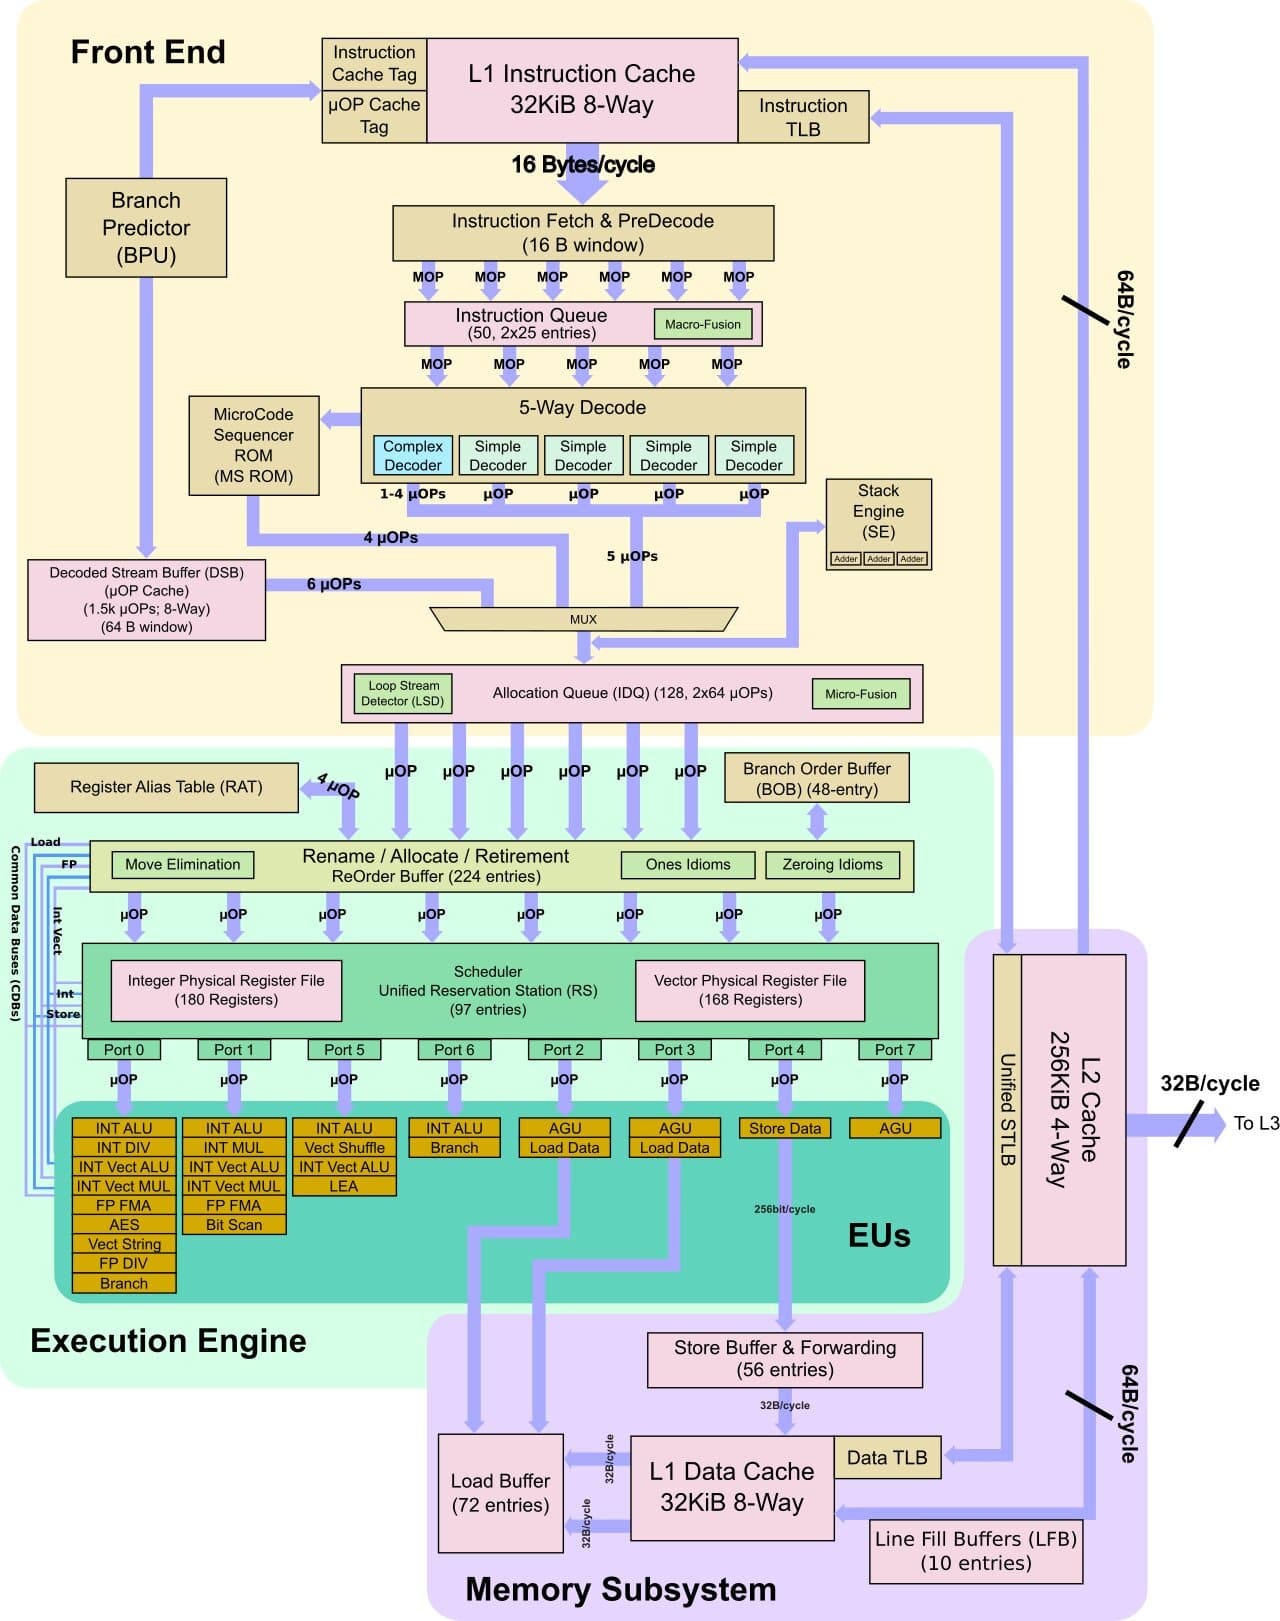
\includegraphics[width=5cm]{DayGilles/images/skylake.jpg}
	\end{column}
\end{columns} 
\end{frame}


\begin{frame}[containsverbatim]
\frametitle{Speculative execution }
Speculative execution is a tentative execution \textcolor{red}{despite dependencies}
\vfill
\begin{center}
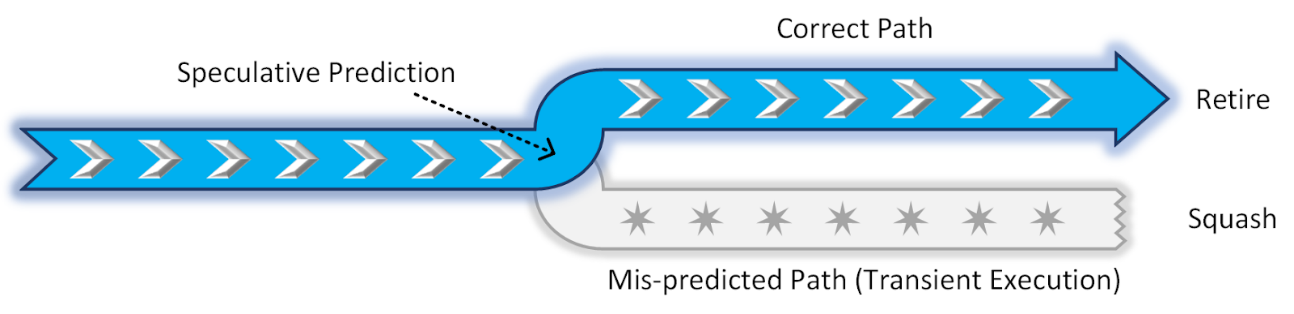
\includegraphics[width=10cm]{DayGilles/images/speculative.png}
\end{center}
\end{frame}


\begin{frame}[containsverbatim]
\frametitle{Data-level parallelism (DLP)}
SIMD = Single Instruction, Multiple Data
\begin{center}
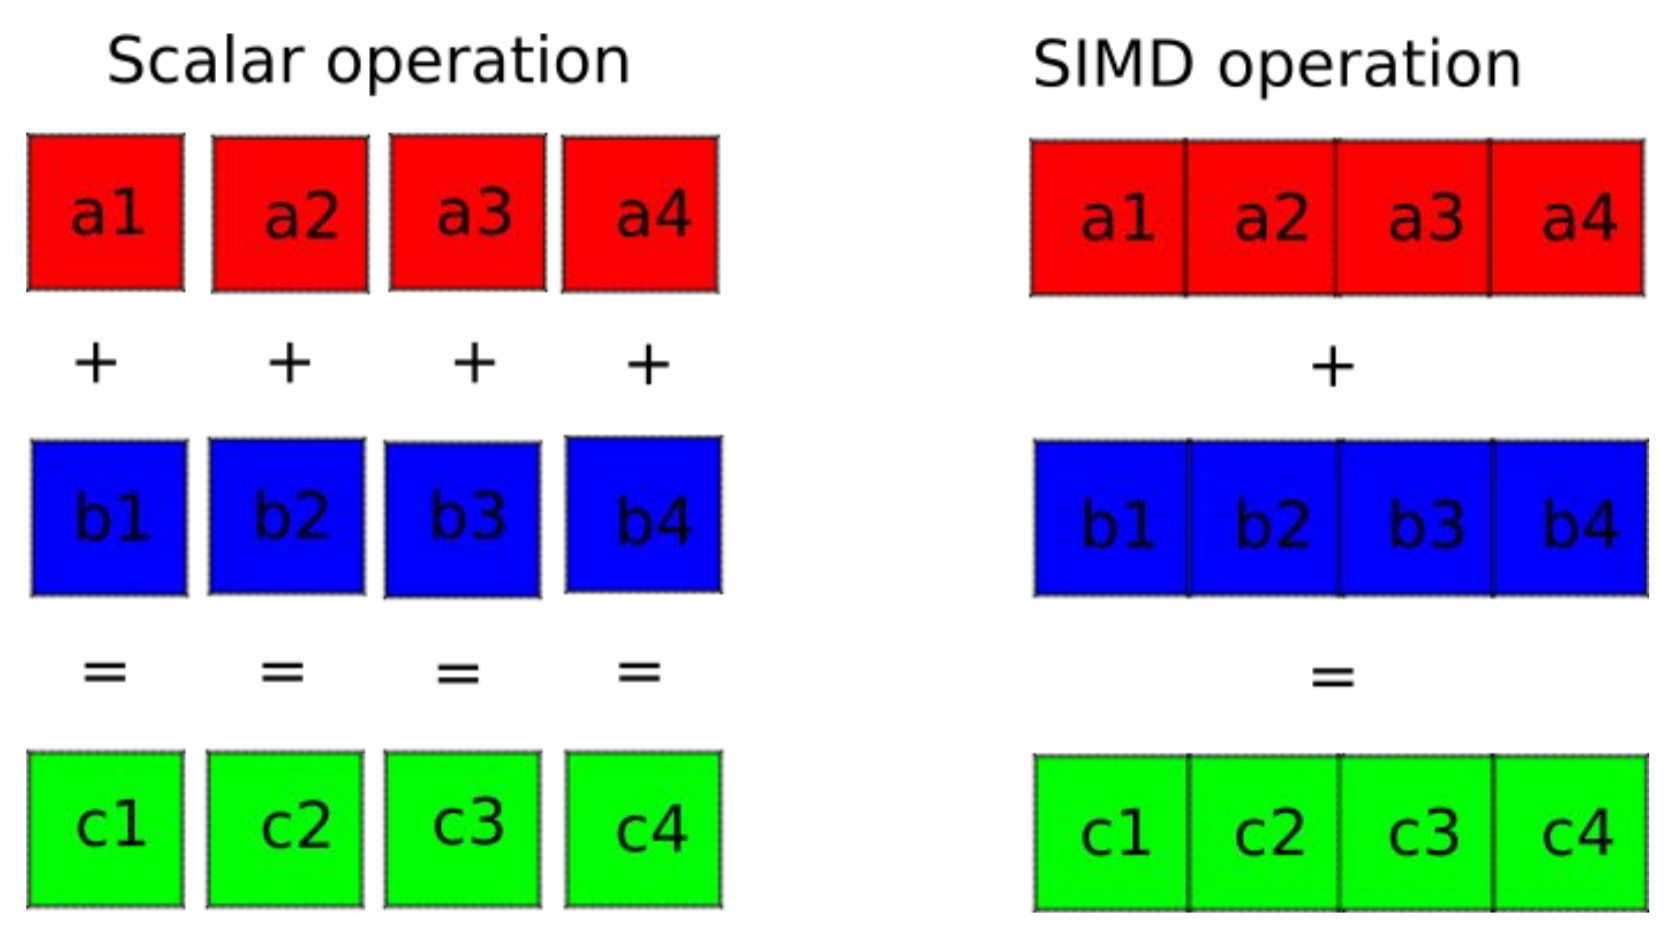
\includegraphics[width=7cm]{DayGilles/images/simd.jpg}
\end{center}
\vfill
\begin{itemize}
\item Throughput is multiplied by the vector size
\item Technologies : Intel AVX (256 bits), Intel AVX512 (512 bits), NVidia GPUs 2048 bits
\end{itemize}
\end{frame}




\begin{frame}[containsverbatim]
\frametitle{HPC data structures: SoA vs. AoS}
\begin{itemize}
\item \textbf{SoA} : Structure of arrays
\item \textbf{AoS} : Array of structures
\end{itemize}
\begin{columns}[c]
	\begin{column}{4cm}
	\begin{lstlisting}[language=C]
struct {
    float a[N];
    float b[N];
    float c[N];
}SoA;
	\end{lstlisting}
	\vfill
	\begin{lstlisting}[language=C]
struct {
    float a,b,c;
} AoS[N];
	\end{lstlisting}
	\end{column} 
	\begin{column}{6cm}
	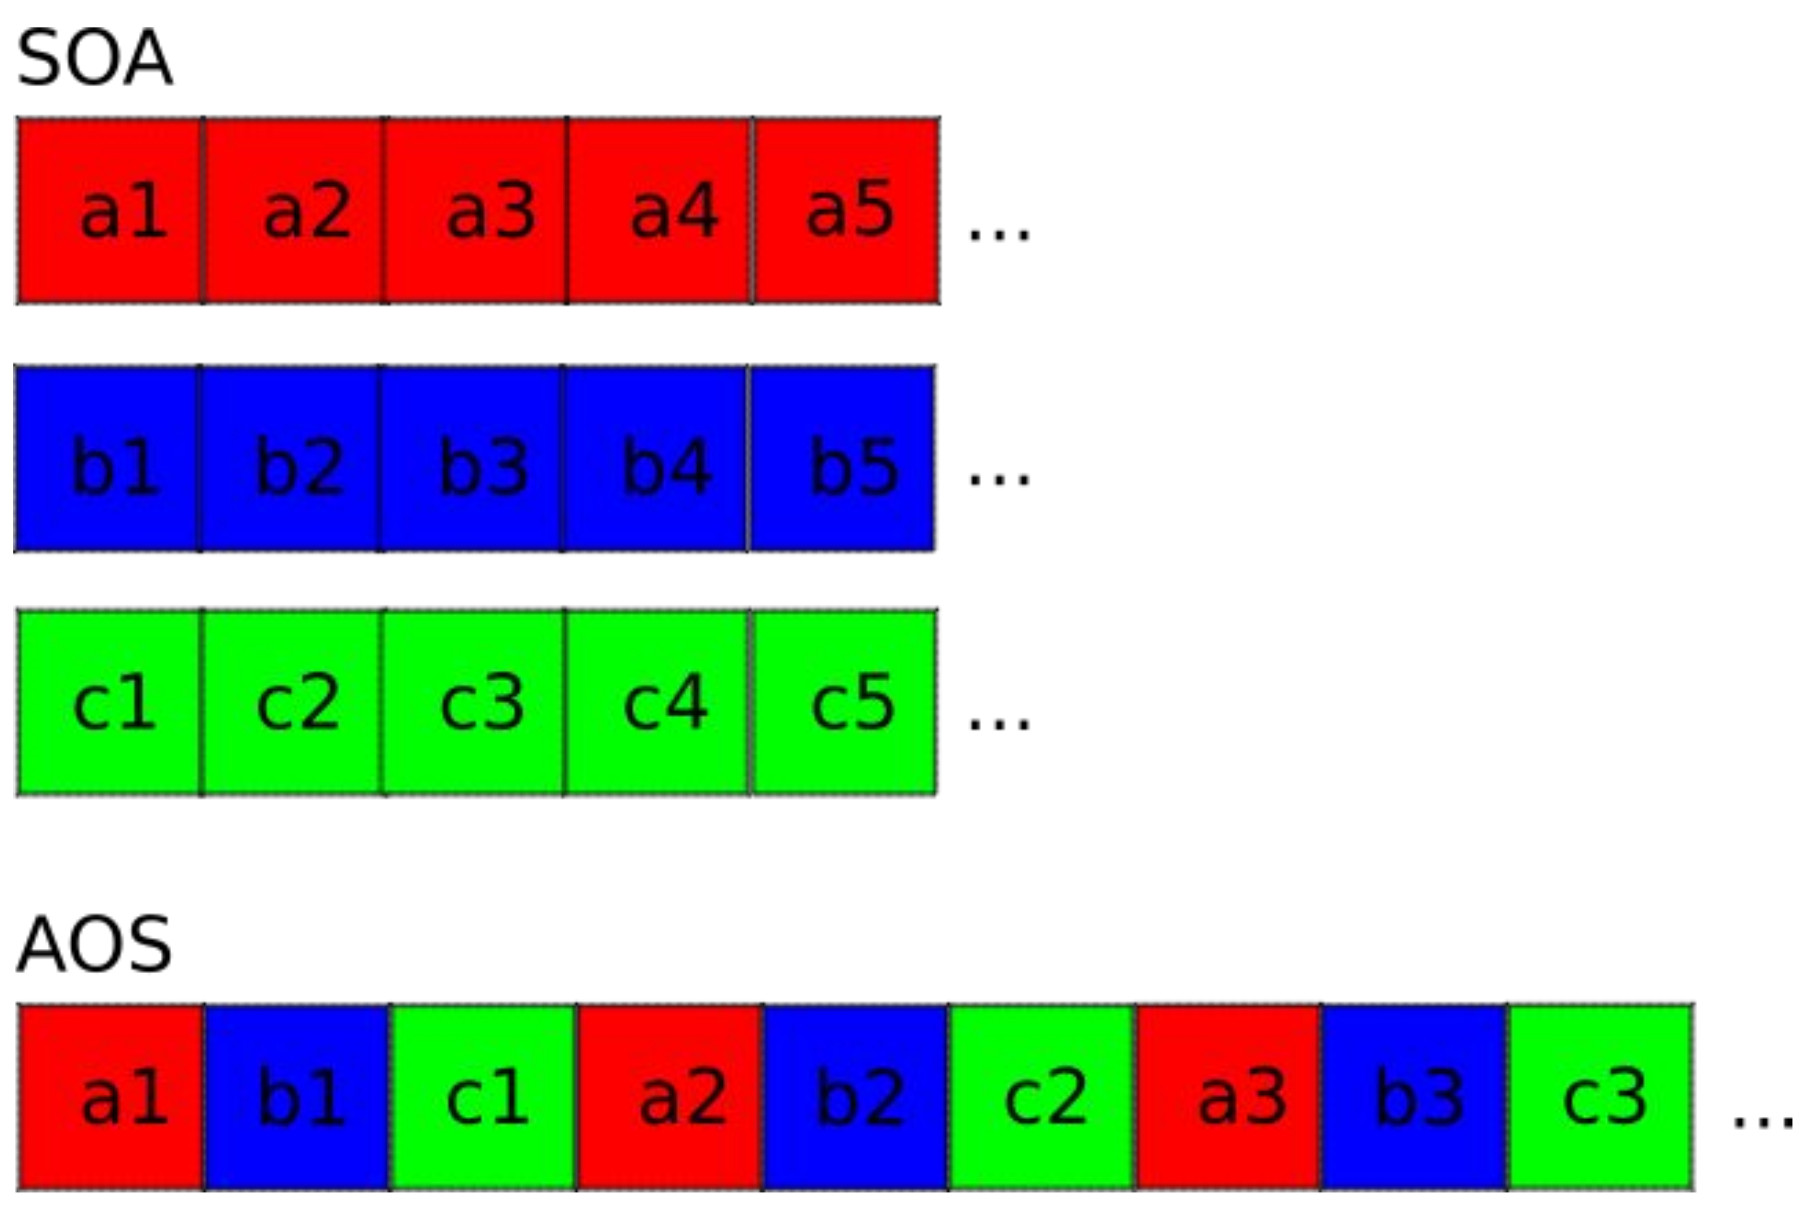
\includegraphics[width=6cm]{DayGilles/images/soa-aos.jpg}
	\end{column}
\end{columns} 
\end{frame}


\begin{frame}[containsverbatim]
\frametitle{HPC data structures: SoA vs. AoS}
\begin{center}
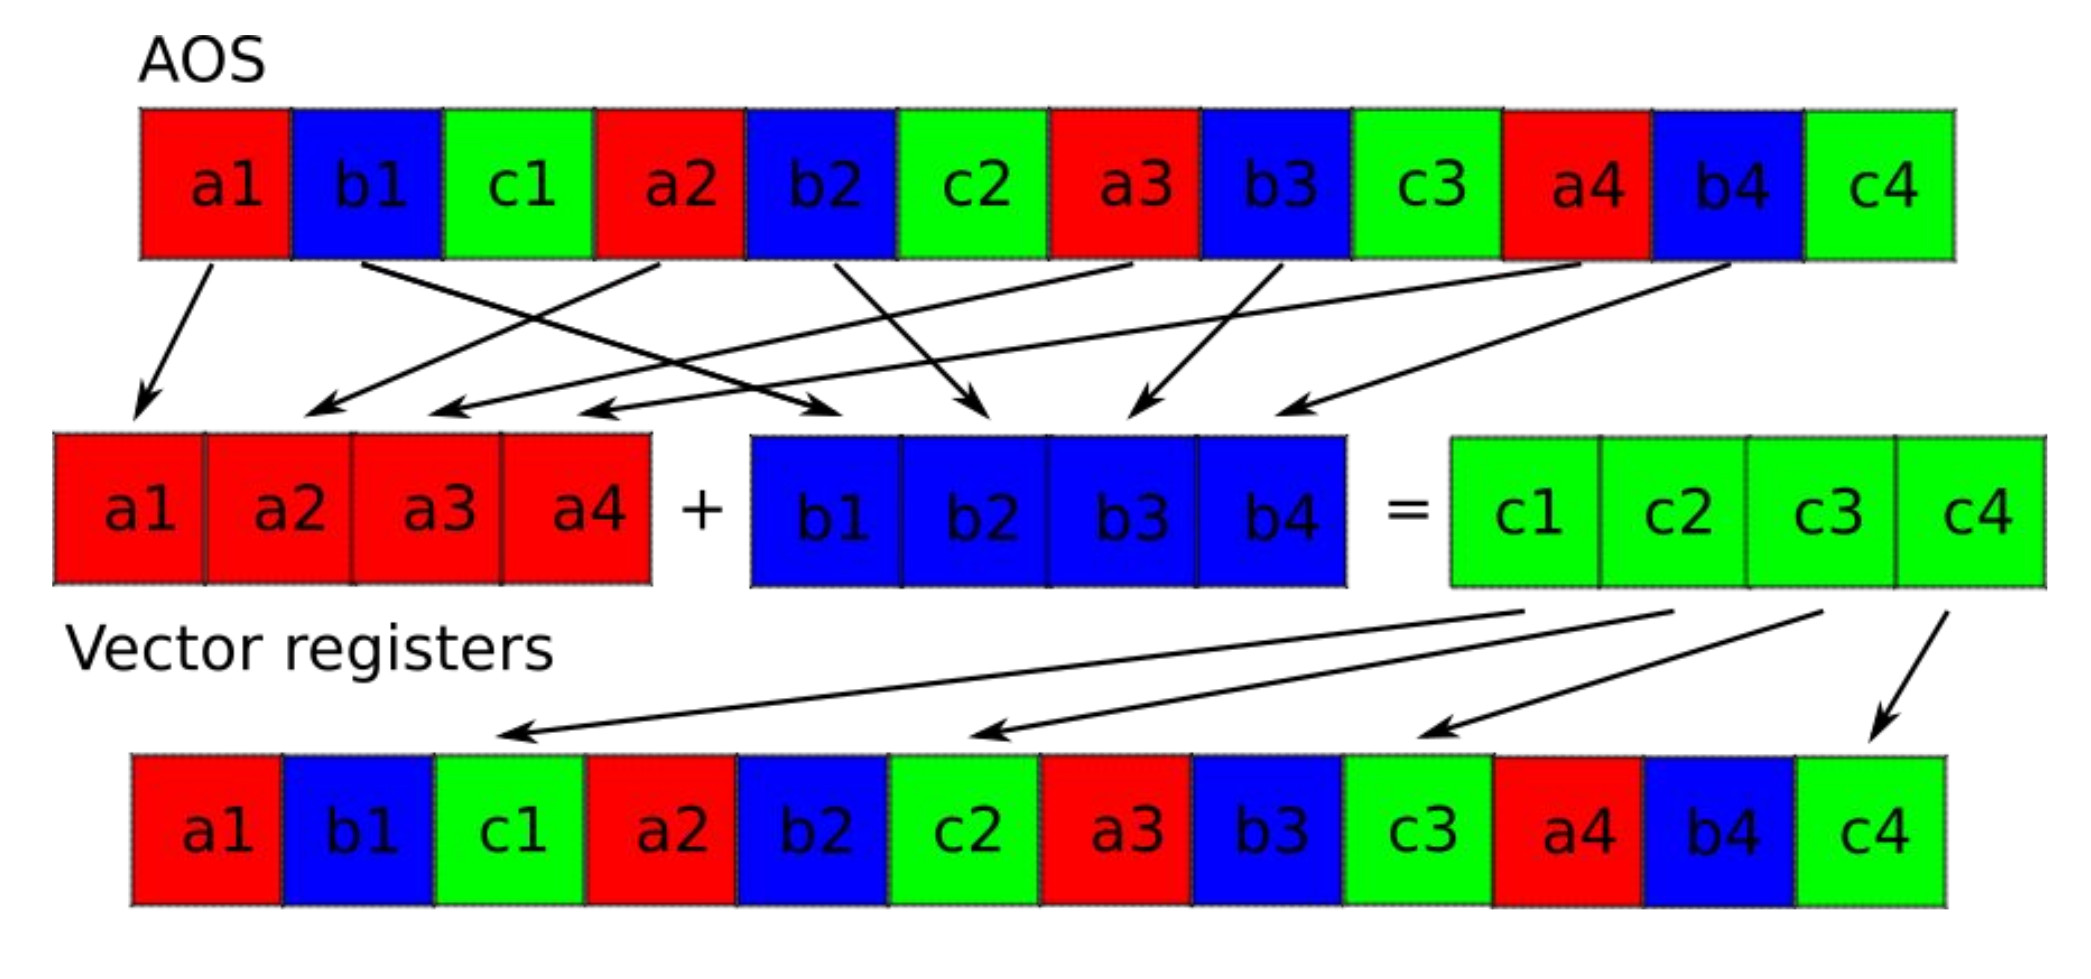
\includegraphics[width=9cm]{DayGilles/images/soa-aos2.jpg}
\end{center}
\begin{itemize}
\item information needs to be shuffled to and from the vector registers before and after the vector operations
\item compilers will have a very hard time in optimizing and vectorizing the code 
\item cache ``unfriendly''
\end{itemize}
\end{frame}

\begin{frame}[containsverbatim]
\frametitle{HPC data structures: SoA vs. AoS}
\begin{center}
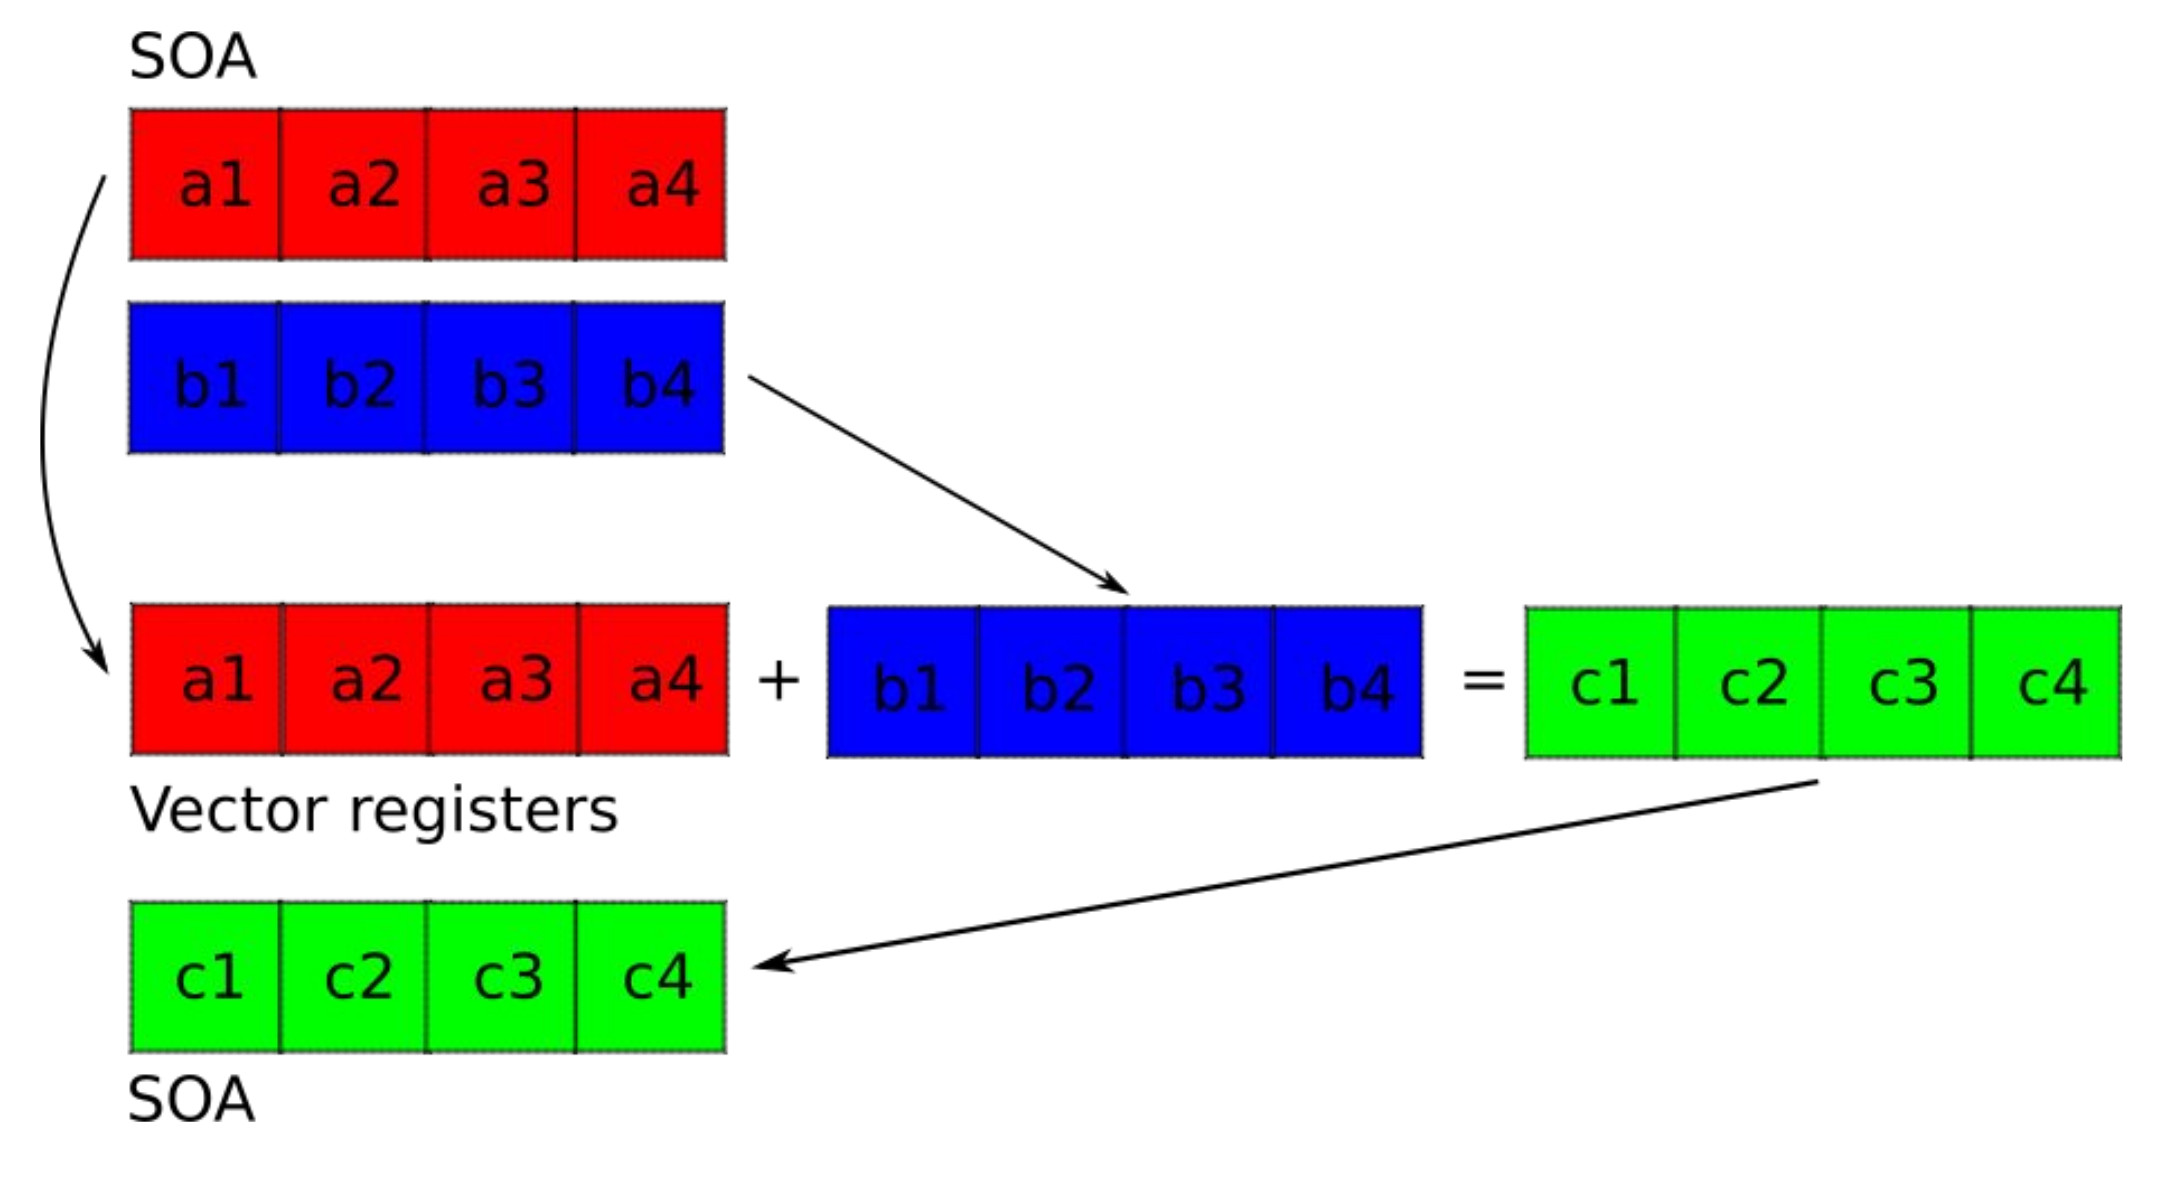
\includegraphics[width=9cm]{DayGilles/images/soa-aos3.jpg}
\end{center}
\begin{itemize}
\item 1-to-1 correspondance between the cache lines and the registers
\item no shuffle/gather/scatter needed
\end{itemize}
\end{frame}


\begin{frame}[containsverbatim]
\frametitle{DLP compilation and assembly}
{\footnotesize
Compilation flags (for gcc):
\\
Standard optimization flags:
\begin{itemize}
\item \texttt{-O0} : no optimization
\item \texttt{-O1} : enables optimization to reduce time to solution
\item \texttt{-O2} : more agressive optimizations
\end{itemize}
Standard debug flags :
\begin{itemize}
\item \texttt{-g0} : no debug information
\item \texttt{-g1} : minimal debug information
\item \texttt{-g} : default debug information
\item \texttt{-g3} : maximal debug information
\end{itemize}
Special flag \texttt{-Ofast}
\begin{itemize}
\item sets \texttt{-O3}
\item sets \texttt{-fast-math}, extra performance boost you need but : breaks struct IEEE-754 (FP), reorder instructions to improve ILP, enables fast approximations of transcendental functions (sqrt, div, ...)
\end{itemize}
}
\end{frame}



\begin{frame}[containsverbatim]
\frametitle{DLP: compilation and assembly}
\begin{center}
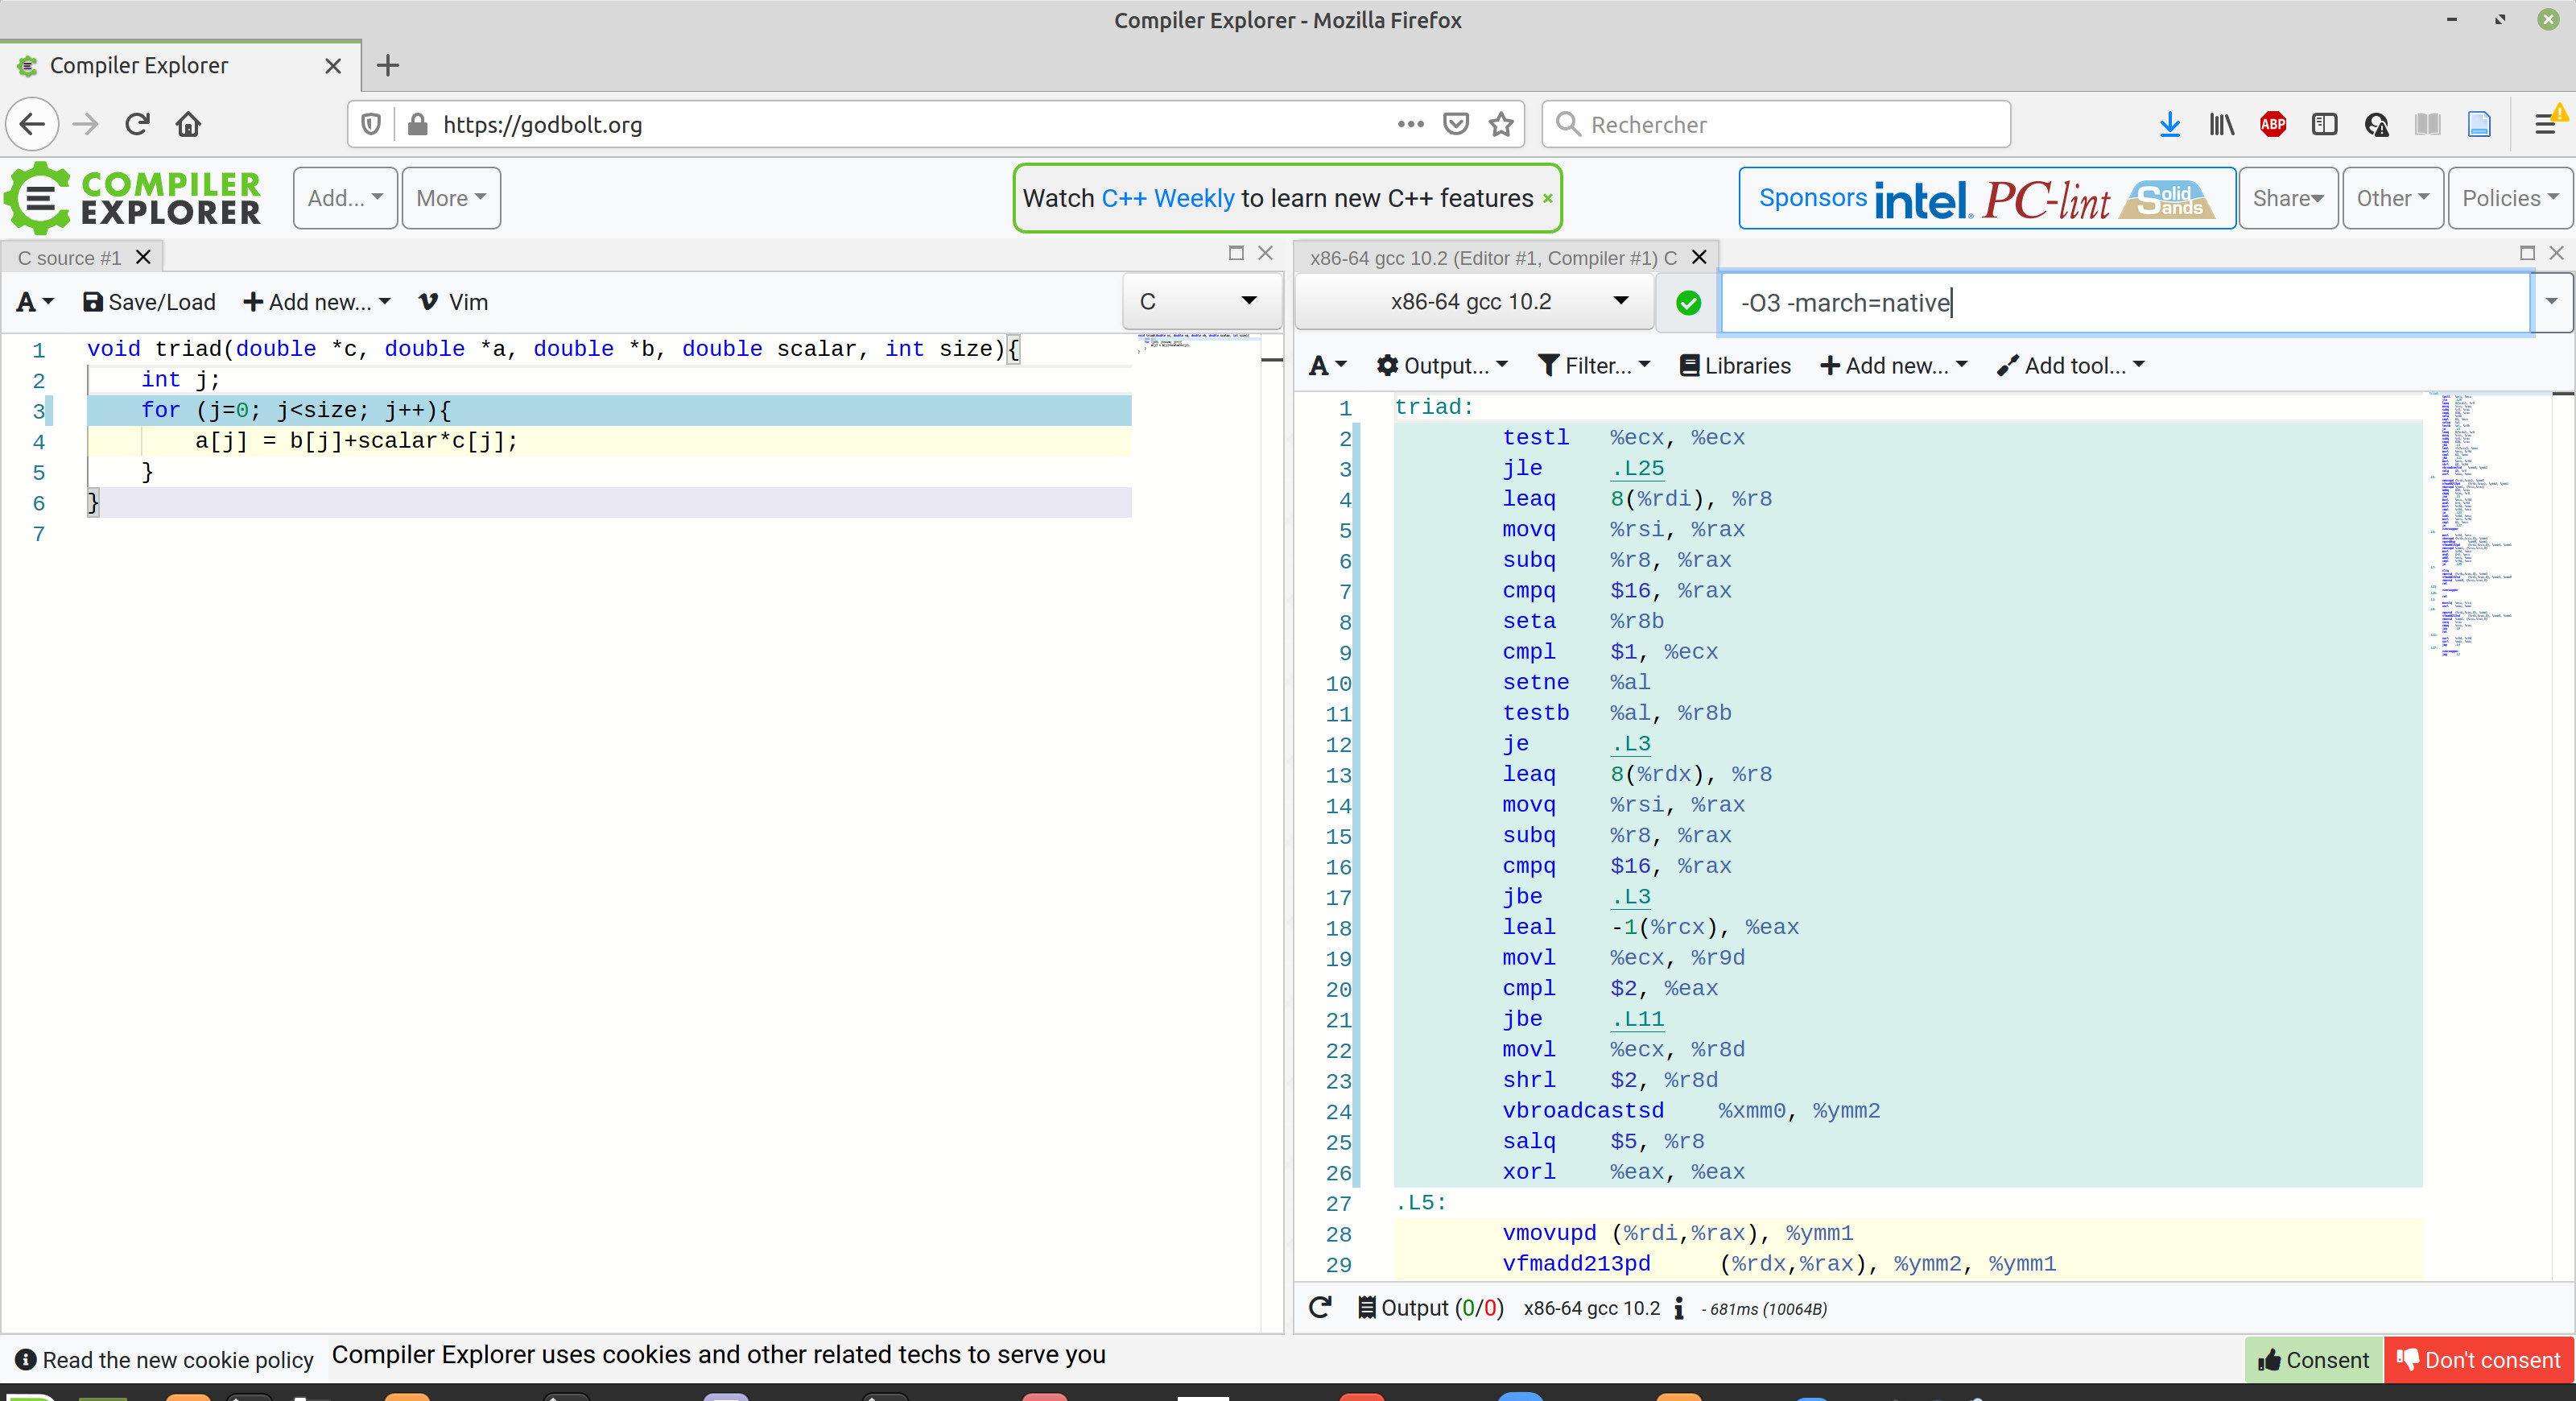
\includegraphics[width=11cm]{DayGilles/images/godbolt.jpg}
\end{center}
{\tiny \url{https://www.gotbolt.org}}
\end{frame}


\begin{frame}[containsverbatim]
\frametitle{DLP: compilation and assembly}
Check the assembly output for vector instructions and registers 
\begin{itemize}
\item compiler option (\texttt{-O3})
\item misalignements
\item standards were not designed for HPC
\end{itemize}
Examples of vector registers :
\begin{itemize}
\item \texttt{xmm} SSE registers : 128 bits
\item \texttt{ymm} AVX registers : 256 bits
\item \texttt{zmm} AVX512 registers : 512 bits
\end{itemize}
Examples of vector instructions :
\begin{itemize}
\item \texttt{vfmadd213pd} : \texttt{v} for vector, \texttt{p} for packed, \texttt{d} for double 
\item \texttt{vfmadd213ss} : first \texttt{s} for scalar, second \texttt{s} for single float.
\end{itemize}
\vfill
{\tiny \url{https://www.gotbolt.org}}
\end{frame}




\begin{frame}[containsverbatim]
\frametitle{TLP : multi/many cores}
\begin{columns}[c]
	\begin{column}{5cm}
{\footnotesize
	Use of multiple concurrent threads that are inherent parallel
	\begin{itemize}
	\item increase throughput of multithreaded codes by covering the latencies
	\item extremly effective in some cases (GPUs)
	\end{itemize}
	However...
	\begin{itemize}
	\item (just) resource (core) duplication
	\item diminishing returns
	\item concurrent programming is very difficult
	\item concurrent hardware is not really designed to support TLP
	\end{itemize}
}
	\end{column} 
	\begin{column}{5cm}
	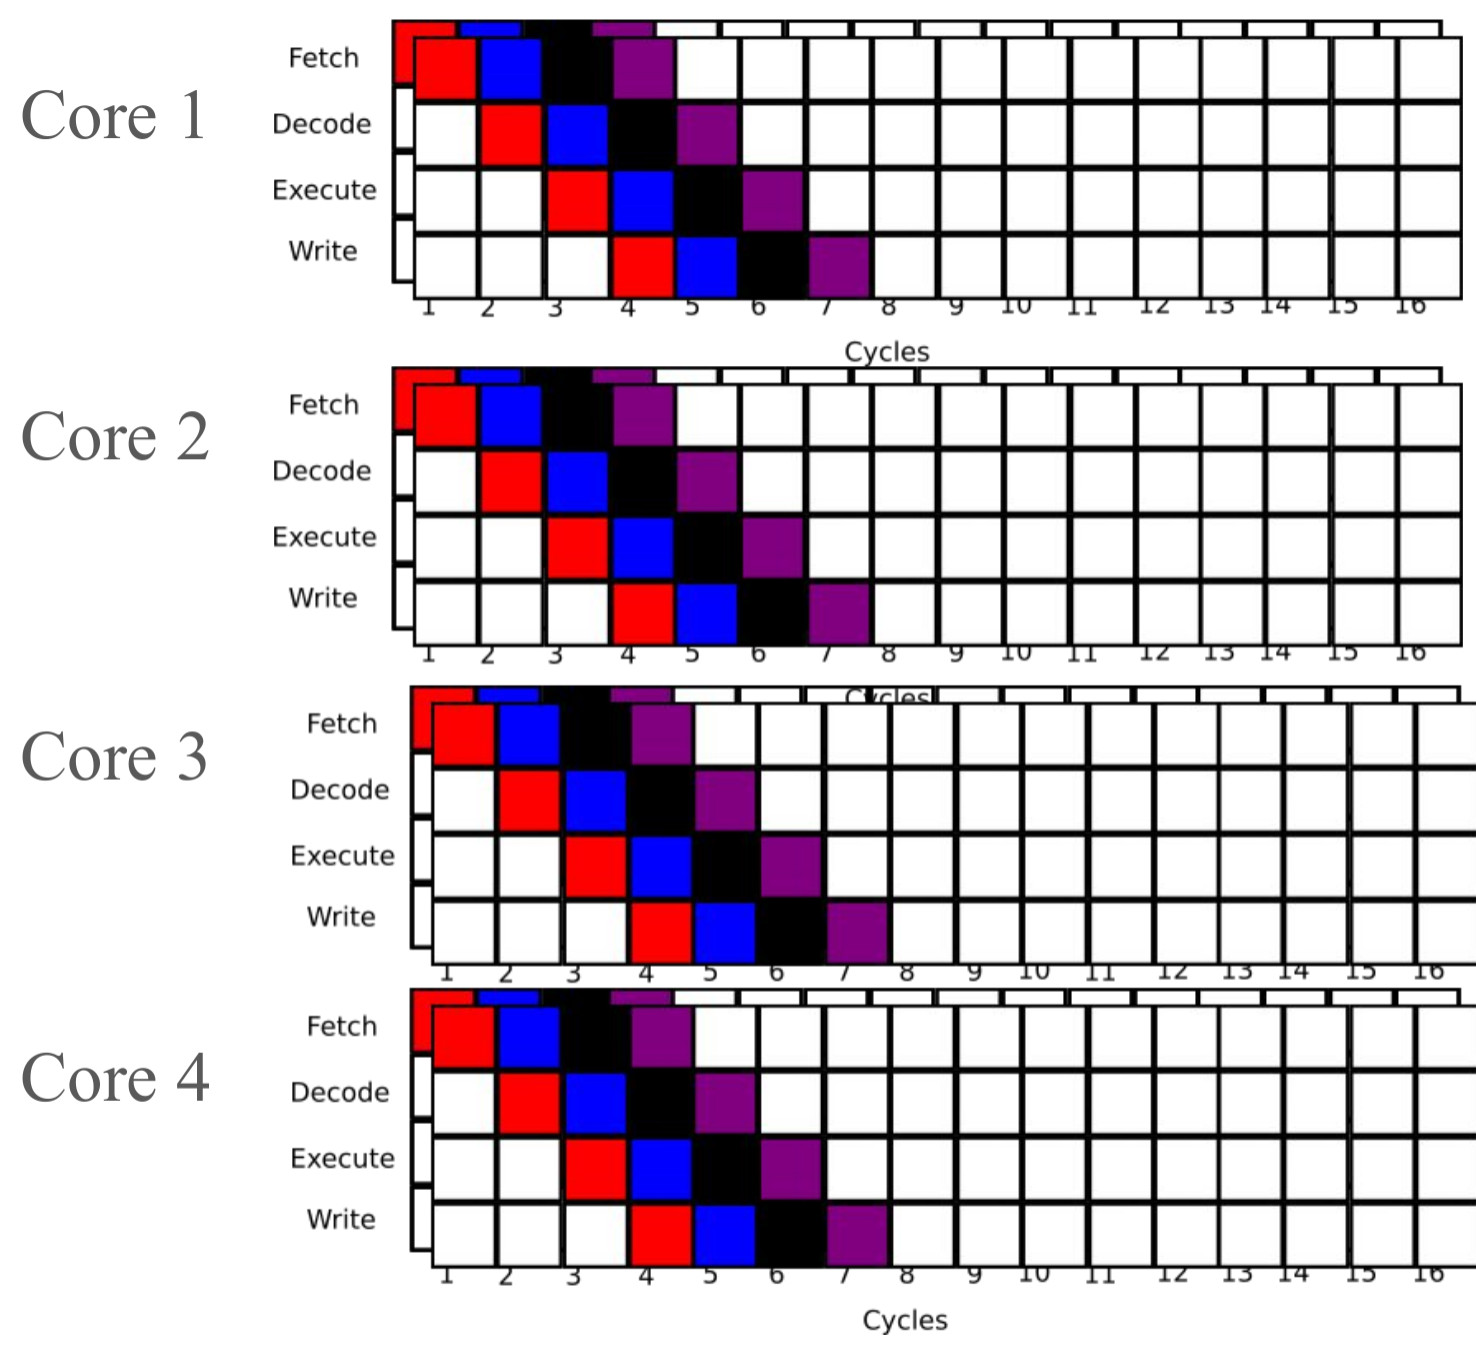
\includegraphics[width=5cm]{DayGilles/images/pipeline-multicores.jpg}
	\end{column}
\end{columns} 
\end{frame}


\begin{frame}[containsverbatim]
\frametitle{HPC Take home message - Node performance}
The goal of HPC is to increase the mathematical throughput
\vfill
\begin{itemize}
\item latency is NOT going down therfore the throughput is increased 
\item throughput is going up IF the parallelism is increased
\item avoid pipeline stalls by having data close to the CPU (in the caches)
\end{itemize}
\vfill
HPC kernel optimization focus on \textcolor{red}{extracting parallelism} and \textcolor{red}{maximizing data locality}
\end{frame}



\begin{frame}[containsverbatim]
\frametitle{Assessing performance : the roofline model}
\begin{itemize}
\item There are many different types of hardware (CPUs, GPUs, ...)
\item There are many different codes (algorithms, kernels, ...)
\end{itemize}
Is there a unified model to assess software performance ?
\vfill
\begin{center}
\textbf{Answer : the roofline model}
\end{center}
\vfill
{\tiny
\begin{itemize}
\item Roofline: an insightful visual performance model for multicore architectures, Williams, S. and Waterman, A. and Patterson, D.,
Communication to ACM, 2009
\item A view of the parallel computing landscape, K. Asanovic, R. Bodik, J. Demmel, T. Keaveny, K. Keutzer, J. Kubiatowicz, N. Morgan, D.
Patterson, K. Sen, J. Wawrzynek, D. Wessel, and K. Yelick, Communication to ACM, 2009
\end{itemize}
}


\end{frame}


\begin{frame}[containsverbatim]
\frametitle{Assessing performance : the roofline model}
Software abstraction. Kernels can be represented by :
\begin{itemize}
\item the number of mathematical operations (Flops)
\item the number of data transfers (B)
\end{itemize}
\vfill
Hardware abstraction. Time-to-Solution is inversely proportional to :
\begin{itemize}
\item the mathematical throughput(Flops/s)
\item DRAM throughput (B/s)
\end{itemize}
\end{frame}


\begin{frame}[containsverbatim]
\frametitle{Assessing performance : the roofline model}
\textbf{Arithmetical intensity (AI)}
\vfill
\begin{columns}[c]
	\begin{column}{5cm}
	\textcolor{red}{AI = Flops/DRAM accesses}
	\\
	The performance of a kernel is the minimum of
	\begin{itemize}
	\item peak FP performance
	\item peak BW * \textcolor{red}{AI}
	\end{itemize}
	Measures :
	\begin{itemize}
	\item peak FP using DGEMM (BLAS3)
	\item peak BW using STREAM
	\end{itemize}

	\end{column} 
	\begin{column}{5cm}
	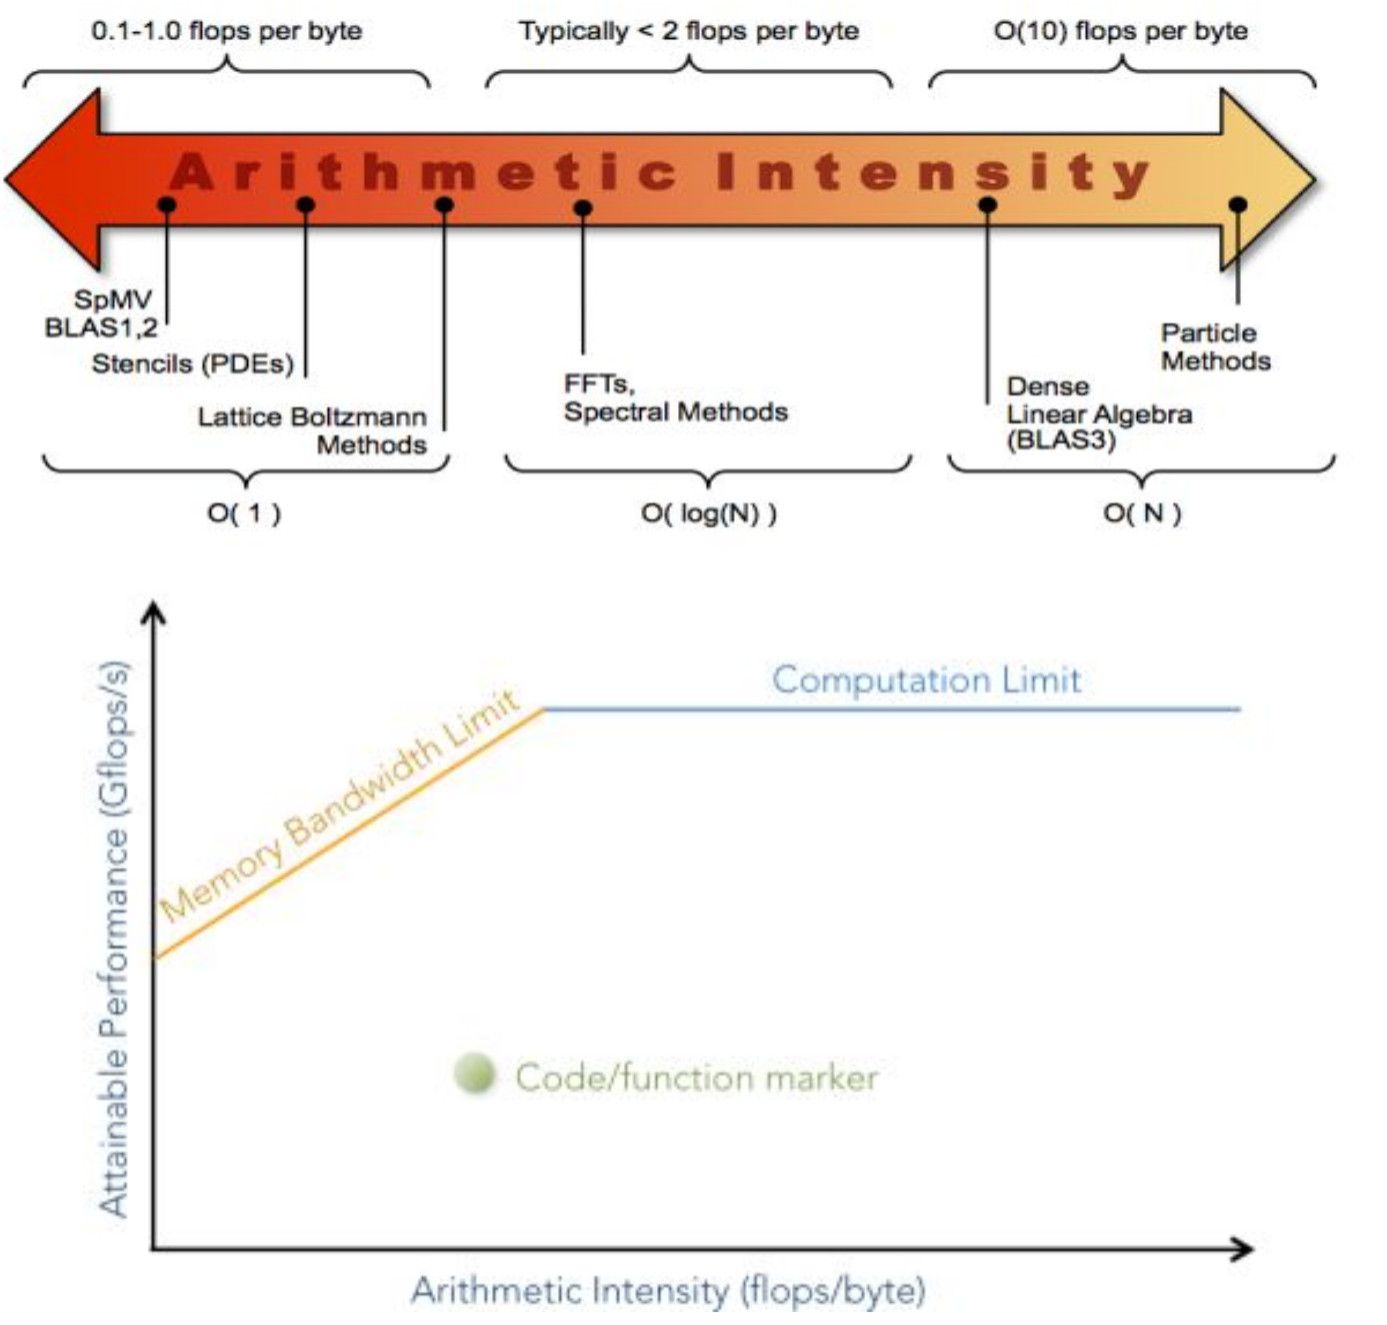
\includegraphics[width=5cm]{DayGilles/images/ai.jpg}
	\end{column}
\end{columns} 
\end{frame}


\begin{frame}[containsverbatim]
\frametitle{Assessing performance : the roofline model}
\begin{center}
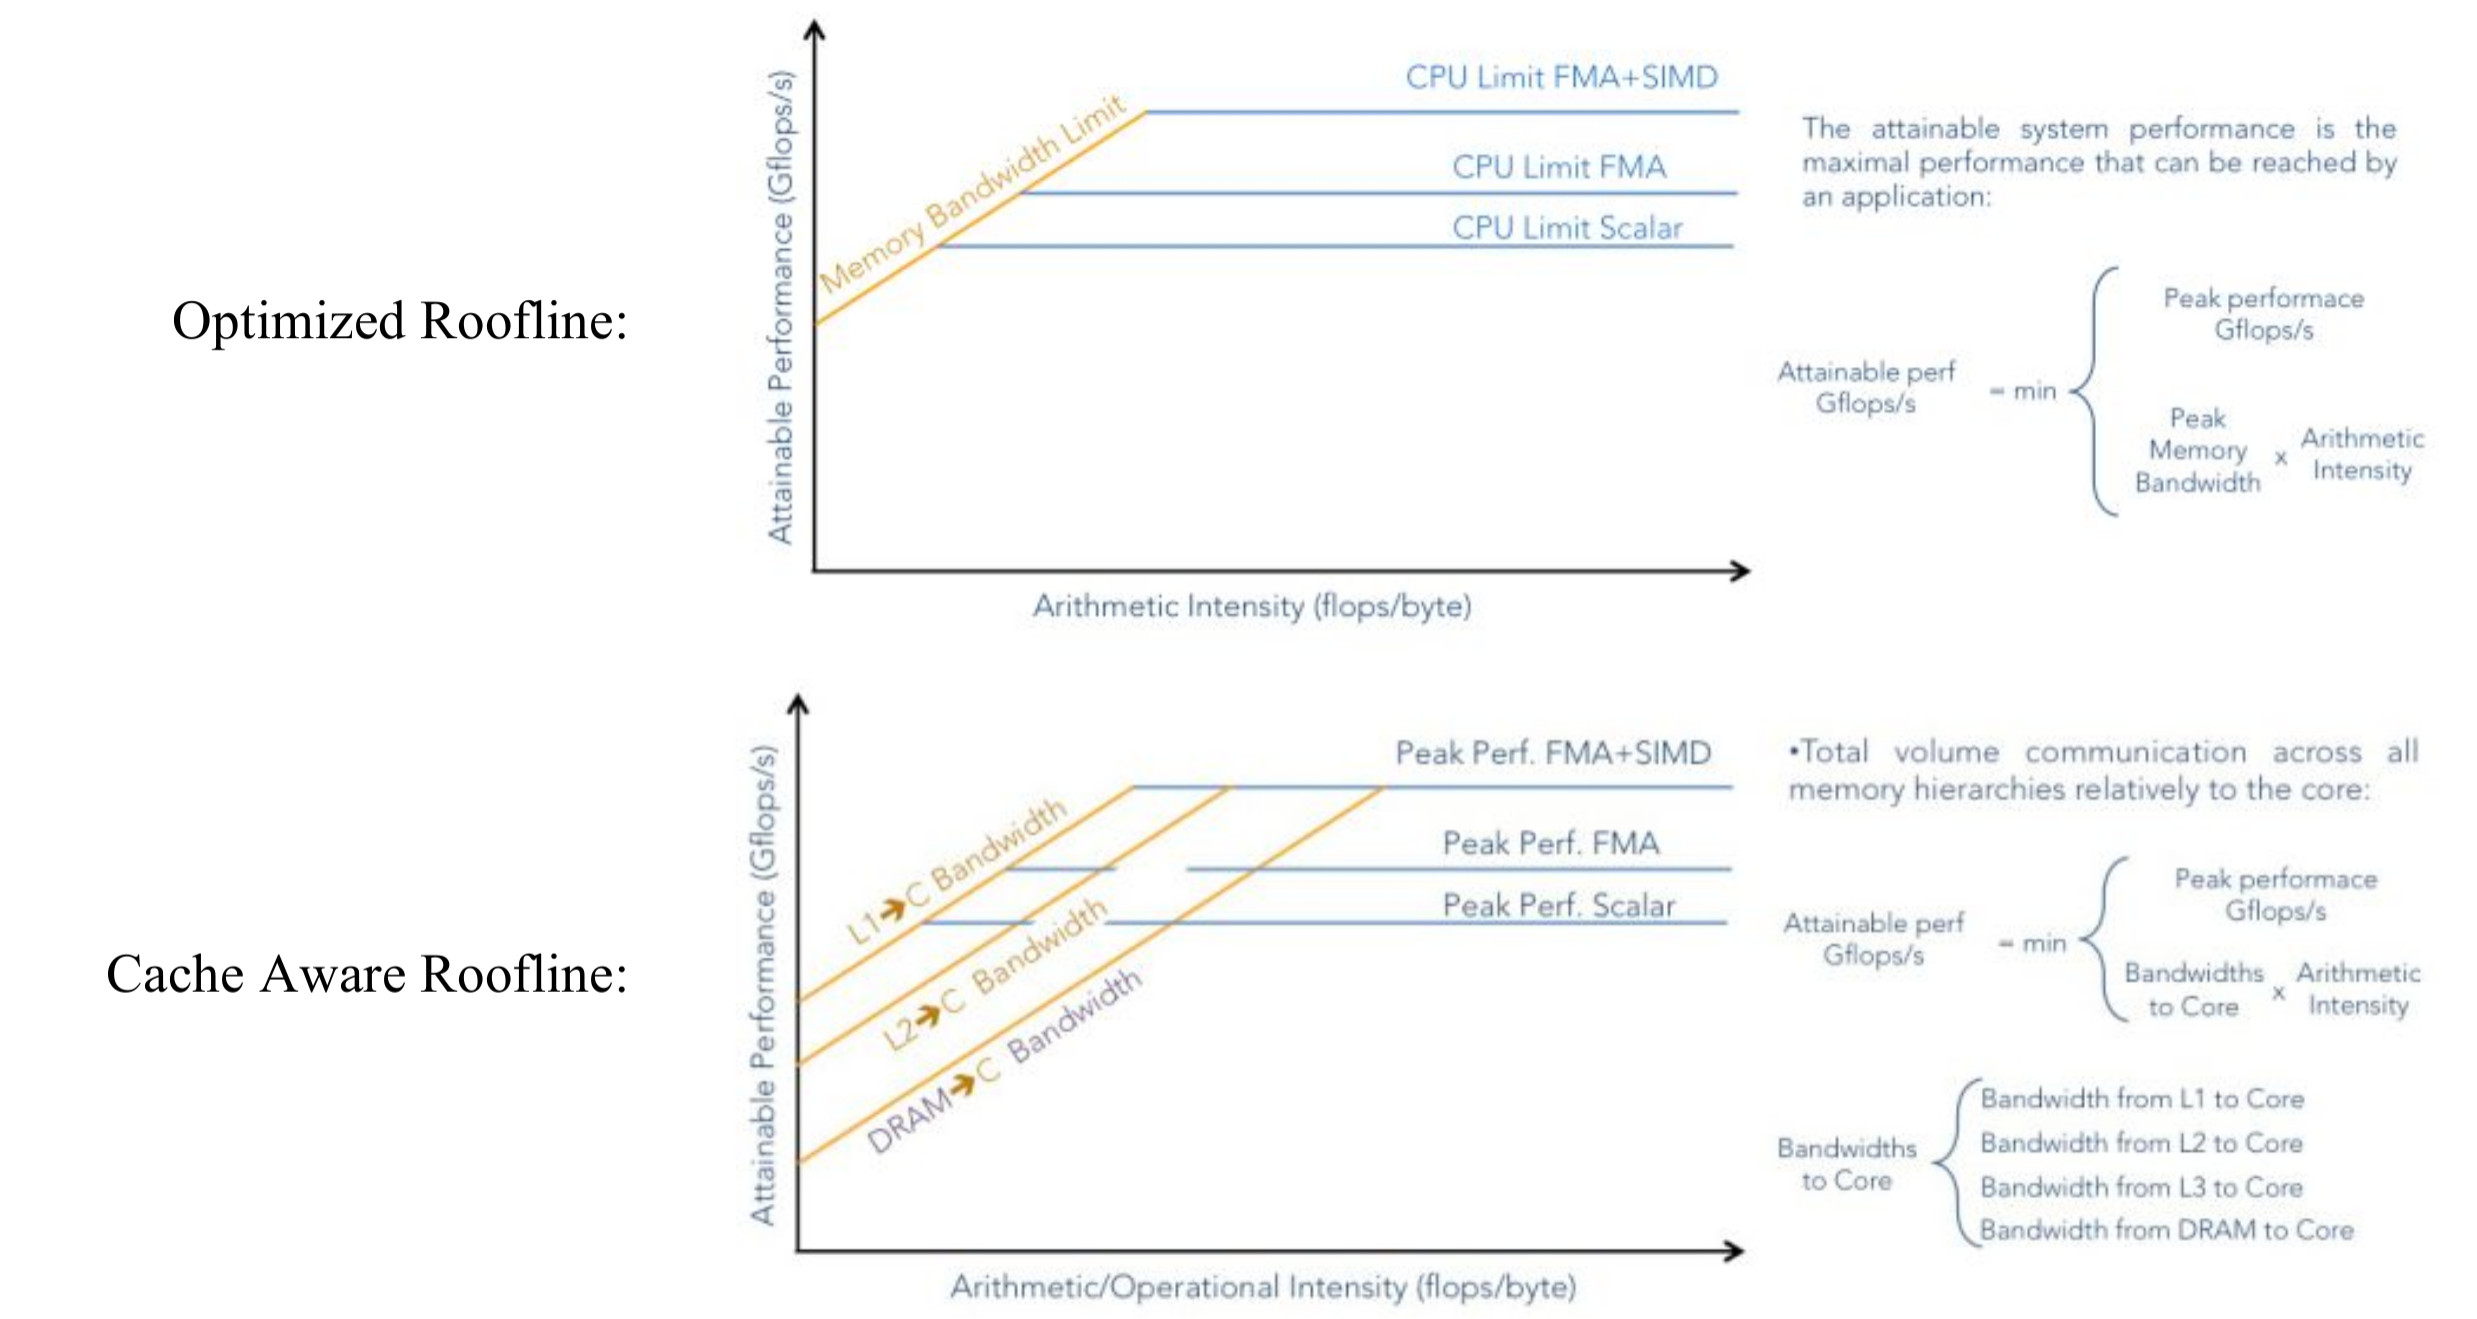
\includegraphics[width=11cm]{DayGilles/images/roofline.jpg}
\end{center}
\end{frame}


\begin{frame}[containsverbatim]
\frametitle{CPU Theoretical peak FP performance }
\begin{tabular}{ r l }
\textbf{Peak performance = } & \textbf{Number of FP ports *} (Superscalar)  \\
& \textbf{flops/cycles *}  (e.g. 2 for FMA) \\
& \textbf{vector size *} (DLP) \\
& \textbf{frequency *} (in GHz) \\
& \textbf{number of cores} (TLP) \\
\end{tabular}
\vfill
Example : Skylake 2.5 GHz, 28 cores (Platinium 8180)
\begin{tabular}{ r l }
\textbf{Peak performance = } & \textbf{2 *} (Superscalar architecture)  \\
& \textbf{2 *}  (FMA) \\
& \textbf{8 *} (DLP) \\
& \textbf{2.5 *} (frequency) \\
& \textbf{28} (cores) \\
\textbf{=}&\textbf{2240} GFlops/s DP per socket (CPU) \\
\end{tabular}
\end{frame}


\begin{frame}[containsverbatim]
\frametitle{Assessing performance : the roofline model}
\textbf{Advantages}
\begin{itemize}
\item caps the performance
\item allows visual goals for optimization 
\item easily used everywhere 
\end{itemize}
\vfill
\textbf{Disadvantages}
\begin{itemize}
\item latencies need to be covered
\item oversimplification
\item node-only
\item ``vanilla'' version is cache-obvious
\end{itemize}
\end{frame}


\begin{frame}[containsverbatim]
\frametitle{Assessing performance : examples}
Setup:
\begin{itemize}
\item Intel Xeon CPU E5-2680 v3 2.5 GHz
\item DDR3 2.133 GHz
\end{itemize}
Peak performance (1 core) : 2 * 2 * 4 * 2.5 = 40 GFlops/s (34.5 measured)
\\
Peak bandwidth (1 core) : ~20 GB/s (estimation) (13.9 measured)
\vfill
\textcolor{red}{Ridge point : 2 Flops/B, 2.48 measured}
\vfill
\begin{itemize}
\item triad() C function (STREAM)
\item AI: 2 flops/3 * 8 Bytes = 2/24 = 1/12 = 0.083 Flops/B
\item Performance : 13.9 * 0.083 = 1.15 GFlops/s
\end{itemize}
\end{frame}


\begin{frame}[containsverbatim]
\frametitle{Assessing performance : examples}
Setup:
\begin{itemize}
\item Intel Xeon CPU E5-2680 v3 2.5 GHz
\item DDR3 2.133 GHz
\end{itemize}
Peak performance (1 core) : 2 * 2 * 4 * 2.5 = 40 GFlops/s (34.5 measured)
\\
Peak bandwidth (1 core) : ~20 GB/s (estimation) (13.9 measured)
\vfill
\textcolor{red}{Ridge point : 2 Flops/B, 2.48 measured}
\vfill
\begin{itemize}
\item dgemm() C function (BLAS3 : double precision generalized matrix multiplication)
\item AI = 2 * $N^3$ Flops, 3 * $N^2$ * 3 DRAMM accesses = N/12 Flops/B
\item Performance : 34.5 GFlops/s if $N > 2.35 * 3$
\end{itemize}
\end{frame}



\begin{frame}[containsverbatim]
\frametitle{Assessing performance : example (Intel Advisor)}
\begin{center}
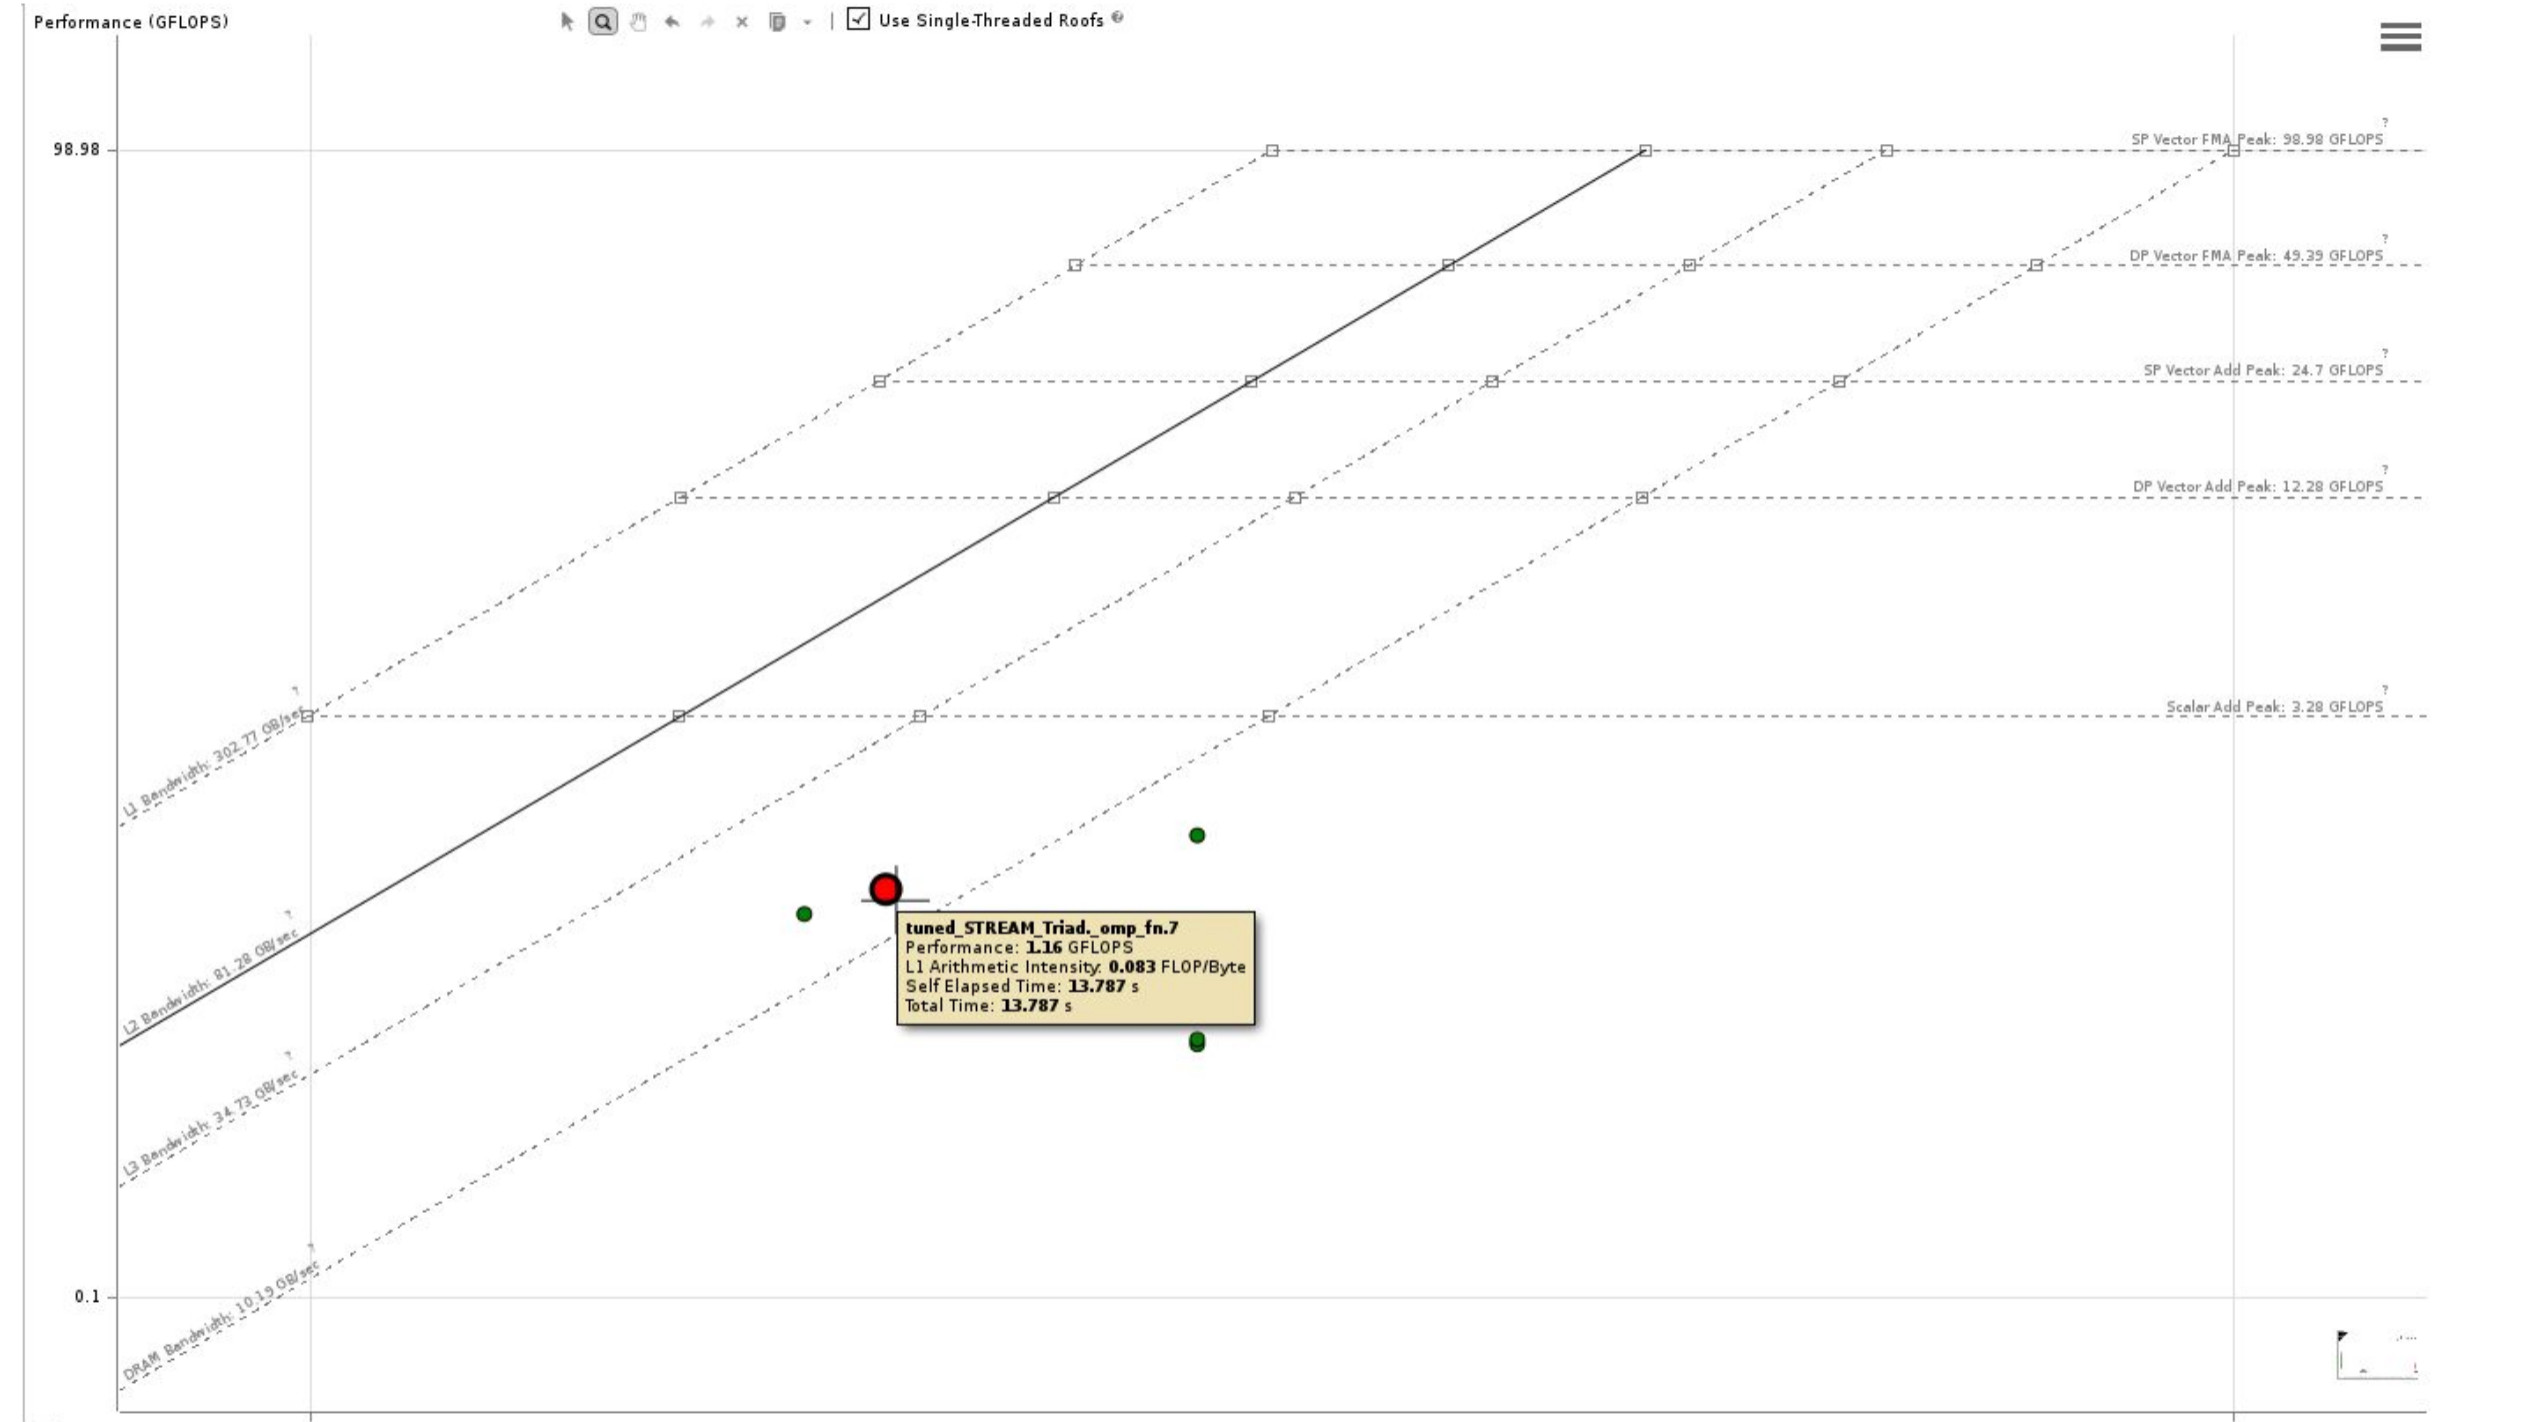
\includegraphics[width=11cm]{DayGilles/images/advisor1.jpg}
\end{center}
\end{frame}



\begin{frame}[containsverbatim]
\frametitle{Assessing performance : example (Intel Advisor)}
\begin{columns}[c]
	\begin{column}{7cm}

	\textbf{DGEMM} : \textbf{D}ouble precision \textbf{GE}neralized \textbf{M}atrix \textbf{M}ultiplication (BLAS3)

\begin{lstlisting}[language=C]
C[i,j] += sum(A[i,k] * B[k,j])
\end{lstlisting}

Arithmeric Intensity :
\\

2 * $N^3$ Flops, 3 * $N^2$ * 8 DRAM access $\rightarrow$ $\frac{N}{12}$ Flops/B
\\

Performance prediction:
\\
34.5 GFlops if $N > 2.35*3$


	\end{column} 

	\begin{column}{3cm}
	\begin{center}
	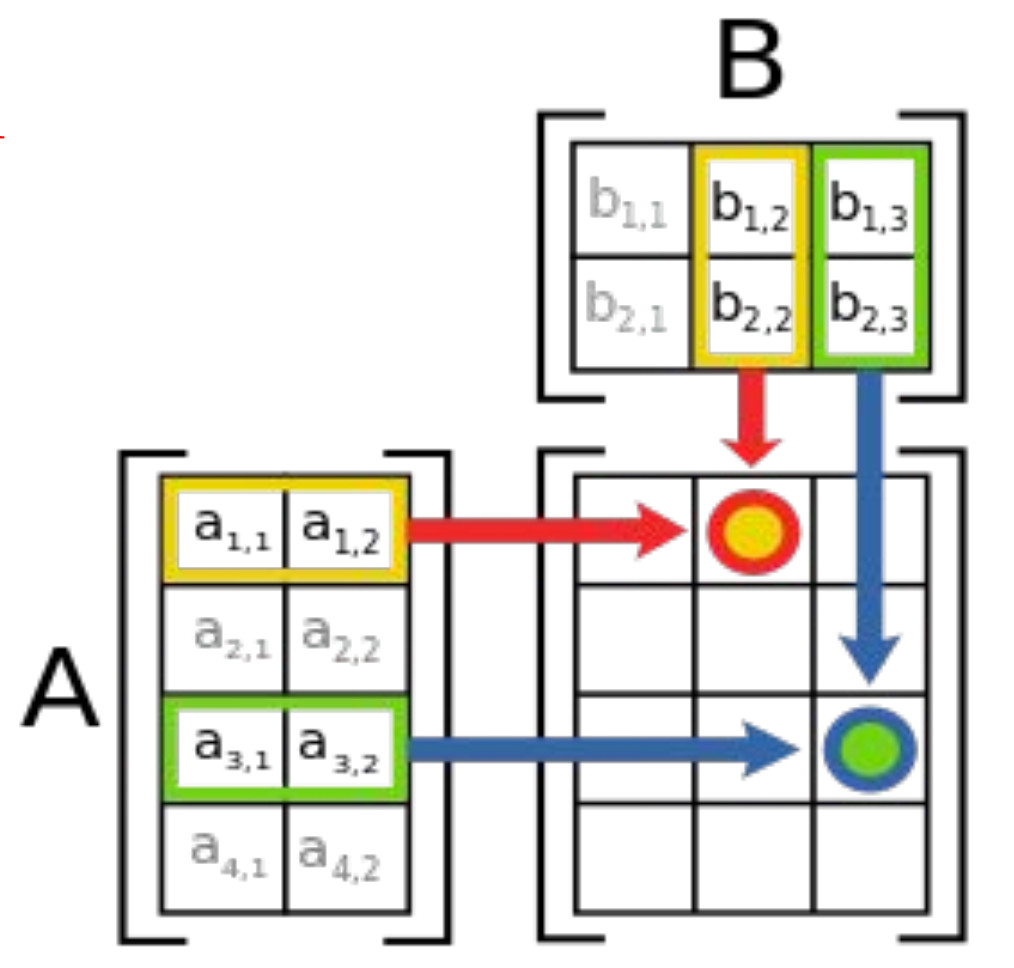
\includegraphics[width=3cm]{DayGilles/images/dgemm.jpg}
	\end{center}
	\end{column}
\end{columns} 
\end{frame}


\begin{frame}[containsverbatim]
\frametitle{Assessing performance : example (Intel Advisor)}
\begin{center}
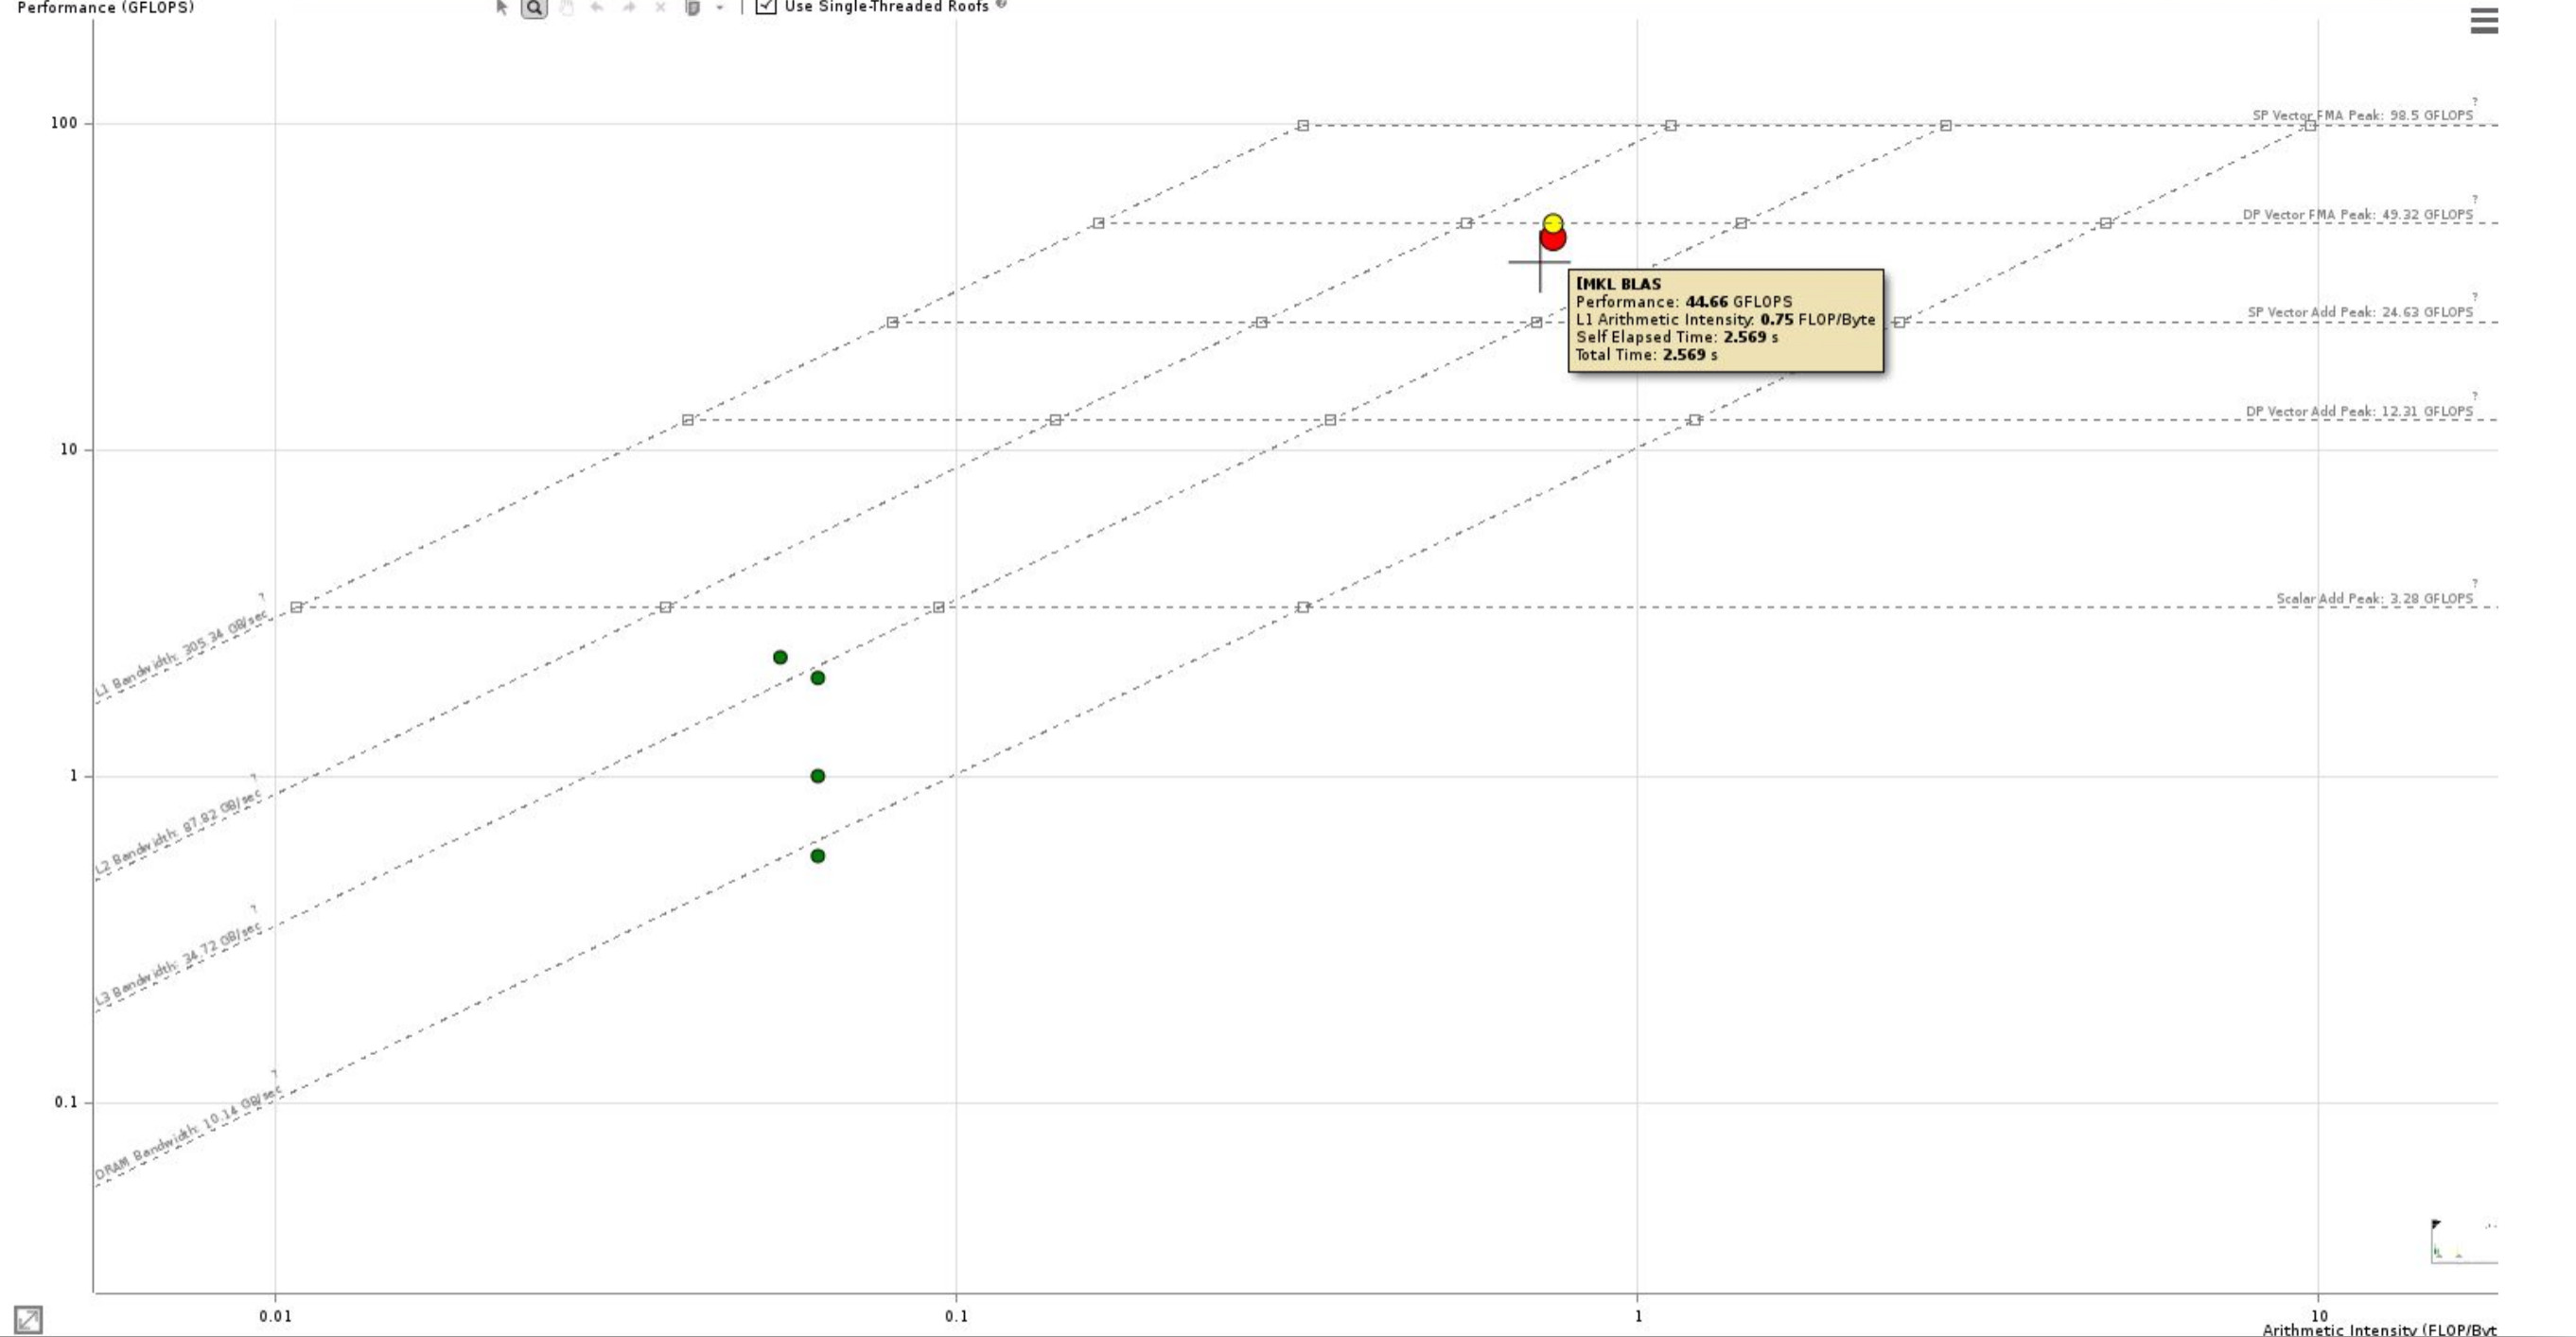
\includegraphics[width=11cm]{DayGilles/images/advisor2.jpg}
\end{center}
\end{frame}


\begin{frame}[containsverbatim]
\frametitle{Assessing performance : Another Go}

\begin{columns}[c]
	\begin{column}{7cm}
{\footnotesize
Flops can be computed by :
\\
Flops/cycle = \# FMA ports * 2 (FMA) * vec length
\\
Ex: Intel XEON E5-2680 v3 2.5 GHz : Flops/cycle = 2*2*4 = 16 Flops/cycle DP
\\
Use RDTSCP on x86\_64:
\\
{\tiny
\begin{lstlisting}[language=C]
static inline unsigned long long cycles()
{
  unsigned long long u;
  asm volatile ("rdtscp; \
    shlq $32, %%rdx; \
    orq %%rdx,%%rax; \
    movq %%rax,%0"\
    :"=q"(u)::"%rax", "%rdx", "rcx");
  return u;
}
\end{lstlisting}
}
and derive performance by counting flops in code
\\
Triad example : 2 (FMA) * 4 (vec length) = 8 Flops in 3 cycles. Performance : 8/3 = 2.6 Flops/cycle, i.e. 6.5 GFlops/s. 
}
	\end{column} 

	\begin{column}{3cm}
	\begin{center}
	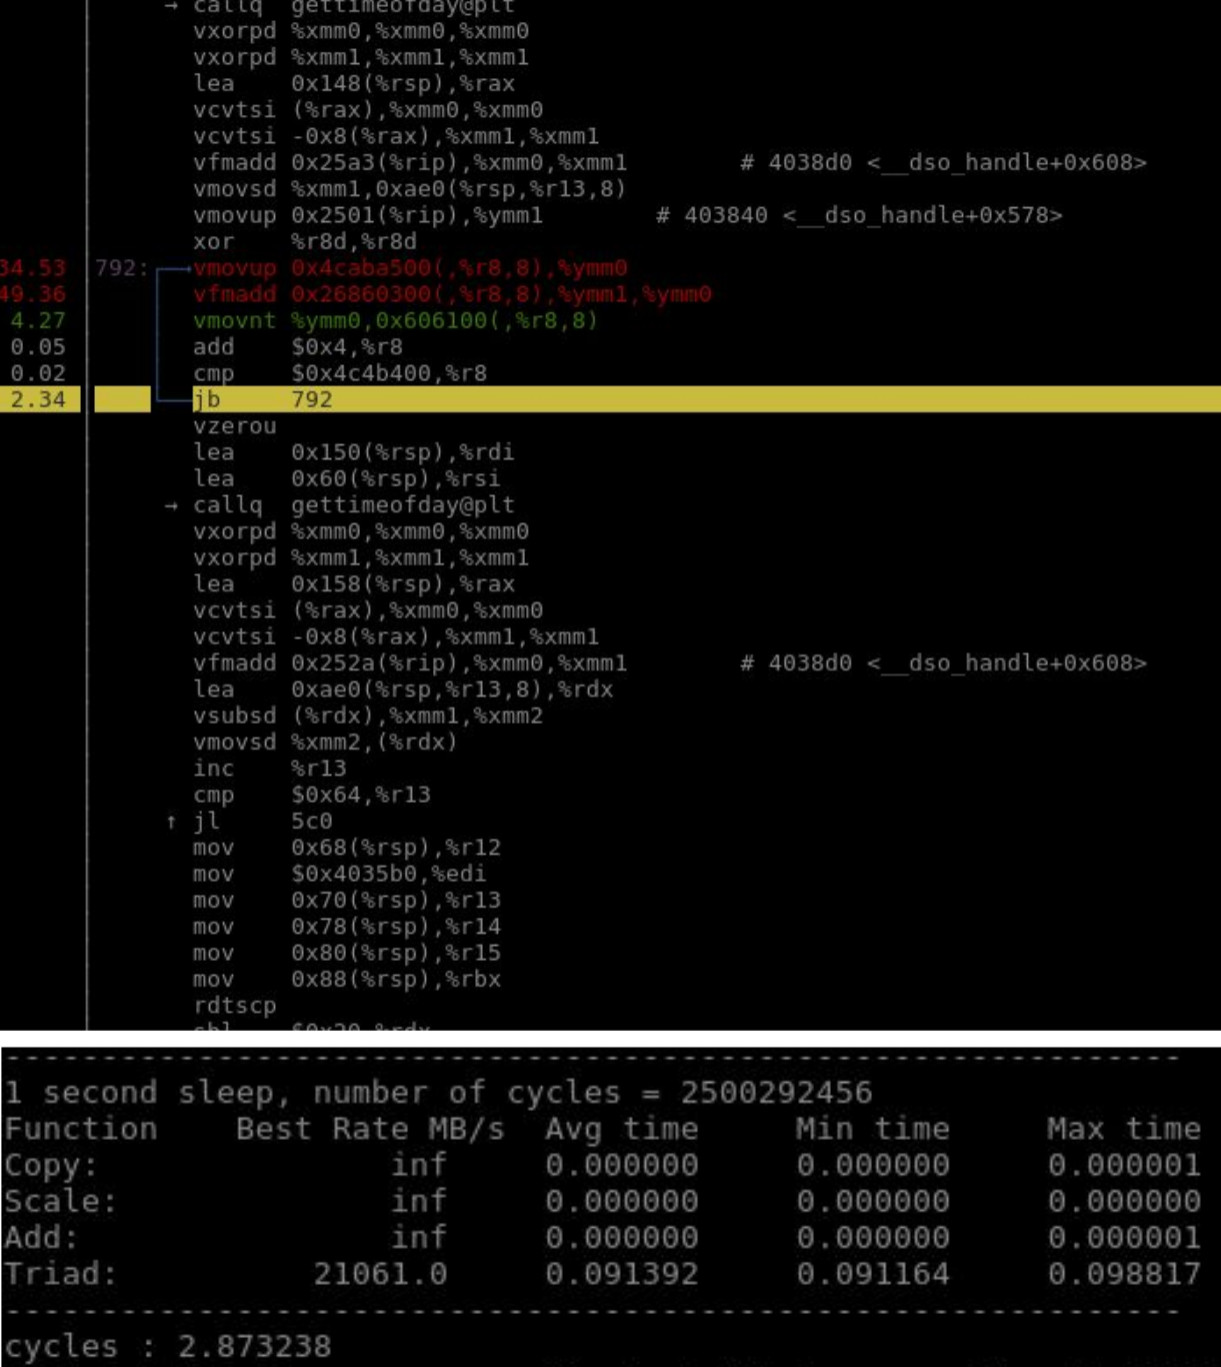
\includegraphics[width=3cm]{DayGilles/images/anothergo.jpg}
	\end{center}
	\end{column}
\end{columns} 
\end{frame}



\begin{frame}[containsverbatim]
\frametitle{Floating point representation}

{\footnotesize
All real number can be approximated by floating point number represented by :
$$
(a-)^s d.dd.... d \times \beta^e
$$
where :
\begin{itemize}
\item $d.dd.... d$ is called \textbf{mantissa} and has $p$ digits : $d.dd.... d =  (d_0 + d_1 \beta + d_2 \beta^2 + ... + d_{p-1} \beta^{p-1})$
\item $\beta$  is the base
\item $e$ is the exponent
\item $s$ is the sign
\end{itemize}

Any real number can be represented by a linear combination of $0.5, 0.25, 0.125, ... , (1/2^{p-1})$
\\

IEEE 754 defines two different floating point representations : \textbf{single precision} (32 bits) and \textbf{double precision} (64 bits) in base 2:

\begin{center}
\begin{table}
\begin{tabular}{|l|l|l|l|} 
\hline
\textbf{Precision} & \textbf{Sign} & \textbf{Exponent} & \textbf{Mantissa} \\
\hline
Single Precision & 1 & 8 & 23 (+1) \\
\hline
Double Precision & 1 & 11 & 52 (+1) \\
\hline
\end{tabular}
\end{table}
\end{center}
}

\end{frame}



\begin{frame}[containsverbatim]
\frametitle{Floating point representation}
\begin{center}
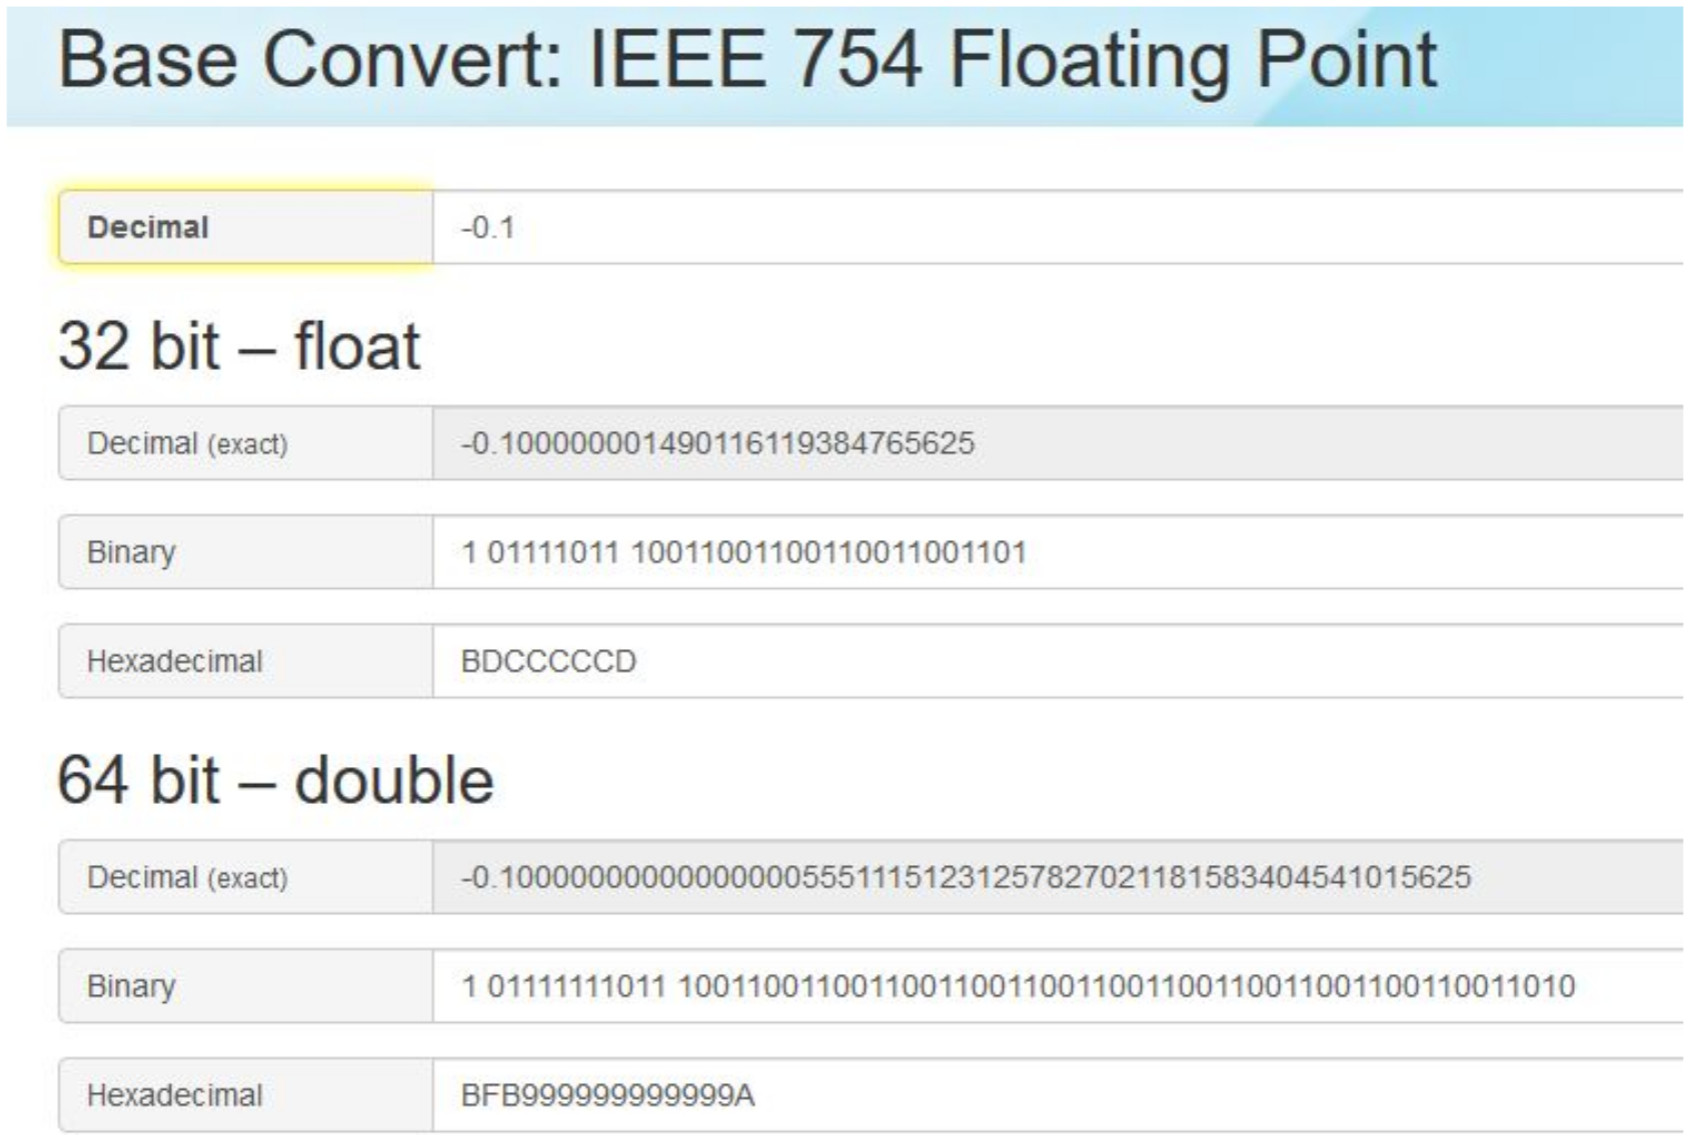
\includegraphics[width=11cm]{DayGilles/images/ieee754.jpg}
\end{center}
\end{frame}



\begin{frame}[containsverbatim]
\frametitle{Floating point representation}
Compute :
$$
f(x,y) = (333.75 - x^2 ) y^6 + x^2 (11 x^2 y^2 - 121 y^4 - 2) + 5.5 y^8 + \frac{x}{2 y}
$$
for :
$$
x = 77617, y = 33096
$$
exactly represented in FP32.

\begin{center}
\begin{table}
\begin{tabular}{ll} 
FP32: & $f(x,y) = 1.1726$ \\
FP64: & $f(x,y) = 1.17260394005318$ \\
FP128: & $f(x,y) = 1.17260394005318631$ \\
\end{tabular}
\end{table}
\end{center}

\textcolor{red}{The correct answer is : $f(x,y) = -0.82739605994682136814116509547981629$}
\\

\textcolor{red}{\textbf{computational precision is not equal to result accuracy !!}}



\end{frame}


\begin{frame}[containsverbatim]
\frametitle{Floating point arithmetic}
${\rm I\!R}$ is a field:
{\footnotesize
\begin{center}
\begin{table}
\begin{tabular}{|l|l|} 
\hline
\textbf{1 - closure}  & \textbf{5 - 0 and 1}  \\
$a + b$ and $a * b$ are in ${\rm I\!R}$ &  $a + 0 = 0 + a$ and $a + 1 = 1 + a$ \\
\hline
\textbf{2 - communitative laws}  & \textbf{6 - $a$ and $-a$}  \\
$a + b = b + a$  and $a * b = b * a$ &  $a + (-a) = (-a) + a$ \\
\hline
\textbf{3 - associative laws}  &  and if $a != 0$ it exists $a^{-1}$ such that \\
$(a + b) + c = a + (b + c)$  and  &  $a * a^{-1} = a^{-1} * a = 1$ \\
$(a * b) * c = a * (b * c)$ & \\
\hline
\textbf{4 - distributive laws}  &  \textbf{7 - it fallows that} \\
$a * (b + c) = a * b + a * c$  and  &  $(a + b) -b = a$ and $a * \frac{b}{a} = b$ \\
\hline
 &  \textbf{8 - cancellation} \\
 & if $a * b = a * c$ and $a != 0$ then $b = c$  \\
\hline
\end{tabular}
\end{table}
\end{center}
}
\end{frame}




\begin{frame}[containsverbatim]
\frametitle{Floating point arithmetic}
\textbf{FP} \textcolor{red}{IS NOT} a field:
{\footnotesize
\begin{center}
\begin{table}
\begin{tabular}{|l|l|} 
\hline
\textbf{1 - closure}  & \textbf{5 - 0 and 1}  \\
$a + b$ and $a * b$ are in FP &  $a + 0 = 0 + a$ and $a + 1 = 1 + a$ \\
\hline
\textbf{2 - communitative laws}  & \textbf{6 - $a$ and $-a$}  \\
$a + b = b + a$  and $a * b = b * a$ &  $a + (-a) = (-a) + a$ \\
\hline
\textbf{\st{3 - associative laws}}  &  and if $a != 0$ it exists $a^{-1}$ such that \\
\st{$(a + b) + c = a + (b + c)$  and}  &  $a * a^{-1} = a^{-1} * a = 1$ \\
\st{$(a * b) * c = a * (b * c)$} & \\
\hline
\textbf{\st{4 - distributive laws}}  &  \textbf{7 - it fallows that} \\
$a * (b + c) = a * b + a * c$  and  &  $(a + b) -b = a$ \st{and $a * \frac{b}{a} = b$} \\
\hline
 &  \textbf{\st{8 - cancellation}} \\
 & \st{if $a * b = a * c$ and $a != 0$ then $b = c$}  \\
\hline
\end{tabular}
\end{table}
\end{center}
}
\end{frame}



\begin{frame}[containsverbatim]
\frametitle{HPC brutal facts}
\begin{itemize}
\item HPC is about minimizing the time to solution (TTS) by \textbf{maximizing the throughput using parallelism}, not reducing latency
\item without HPC techniques, \textbf{your code won't run faster on supercomputers} than on your workstation
\item CPUs are very good at doing \textbf{fused multiply-add (FMA)} but that's about it
\item HPC is about knowing your \textbf{how your software AND your hardware best work together} to get maximum performance
\item HPC is about \textbf{hacking} your ways around the language standard
\item You'll need to have \textbf{a look at the assembly produced}
\end{itemize}
\end{frame}


\begin{frame}[containsverbatim]
\frametitle{Bibliography (to go further...)}
\begin{itemize}
\item \textit{Computer architecture, a quantitative approach}, Patterson, ACM, 2017
\item \textit{Introduction to High Performance Computing for scientists and engineers}, G. Hager, G. Wellin, Champan \& Hall, 2010
\item \textit{Roofline : An insightful visual performance model for multicores architectures}, S. Williams, A. Waterman, D. Patterson, communications of the ACM, 2009
\item \textit{Floating point computation}, Pat. H. Sterbenz, Prentice-Hall series in automatic computation, 1973
\end{itemize}
\end{frame}




